\documentclass[review,onefignum,onetabnum]{siamonline190516}
\usepackage{amsmath,amsfonts,graphicx}
\def\R{\mathbb{R}}
\usepackage{xcolor}
\usepackage{todonotes}
\usepackage{tikz}
\usepackage{array}
\usepackage{natbib}

\date{\today}
\title{Differential invariant signatures for planar Lie group transformations of images}
\author{Not-working authors }

\begin{document}
\maketitle
\begin{abstract}
\end{abstract}


% REQUIRED
\begin{keywords}

\end{keywords}

% REQUIRED
\begin{AMS}

\end{AMS}

\section{Introduction}
\todo[inline]{
Richard: 
Start on invariant tensor theorem
Generate new pictures, add function details
SE(2) jobs inline
Mobius, Conformal -- finish code, tidy writing
First bash at experimental section

Stephen:
Rearrange examples text to IVT section, write about signatures here
Fix up tables, check bib
Examples for SA(2), A(2) -- need to think about sig here
Moving frame intro
Projective -- tidy writing, especially the names of the invariants
Colour
First bash at conclusion

Later:
Introduction
Count of derivatives and what to say
}

\todo[inline]{Examples to be numbered like theorems}
\todo[inline]{This is a start. To be completed later.}

%Biologists differentiate between the {\em form} of an object, and the {\em shape}, being the part of form that is unaffected by size and orientation. 
The appearance of a fixed object in a set of images can vary markedly depending upon such variables as pose and position relative to the camera, even though the object itself does not change. This is even more marked in scenes that consist of multiple objects at different distances and orientations to the camera and any fixed background. The appearance of each individual object will then vary independently as a constant camera motion or other such transformation is applied. Typically the individual transformations will appear as the action of an element of a planar Lie group, for example the affine, or projective groups, or an angle-preserving transformation from the conformal group, depending upon the camera model. %Regardless of which group appears to act, such variations highlight the importance of `shape', as opposed to `form', in object recognition. 

For image recognition it is then natural to seek representations of objects that do not change as these various transformation groups act. If the space of objects is denoted $M$ and the appearance transformations form a group $\mathcal{G}$, then mathematically one seeks a way to study objects in $M / \mathcal{G}$. One way to achieve this is by transforming all objects to match a chosen target object by registration (the transformation of the appearance of one shape to match another, typically by gradient descent on a matching function, see e.g.~\cite{Modersitzki03}). Hence for the group of similarity transformations (rotation and reflection, translation, and scale), a Procrustes alignment~\cite{Kendall1989} will place all of the shapes into the reference frame of one template example. However, analysis on these quotient spaces is rarely simple (see e.g.,~\cite{Marsland19b} for a basic primer), and if one is interested in the object, and not the transformation, then it necessitates a lot of computational work for relatively little benefit. 

An alternative option is to seek $\mathcal{G}$-invariant functions on $M$, which is what we consider here. In this case, rather than considering the image of the object, one constructs an invariant signature of some kind, which represents the object modulo the action of elements from the relevant group. This has been considered extensively by Olver and co-authors for the case of outlines of objects~\cite{Calabi1998,Hoff2013}. In this paper we consider the case of signatures for images rather than curve outlines.

The introduction of an invariant signature reduces the recognition problem to one of comparing the higher-dimensional signatures (typically the signatures need to be at least three dimensional for planar images) that encode the desired self-equivalences. In this paper we introduce the mathematical considerations necessary to construct invariant signatures to the planar Lie groups (and some infinite-dimensional, pseudo-Lie groups too) that can transform 2D images. As we shall show, the lattice structure of the set of groups influences the relationship between the sets of invariants for the different groups. We provide sample signature sets for the various groups we consider, and examples of the appearance of those signatures for transformations of a simple, smooth image, but do not consider the question of a complete practical implementation. We do not consider the classification of the signatures, for which either a standard image recognition algorithm can be used (see, e.g.,~\cite{Zhang20} for a survey), or a matching method such as~\cite{UsCurrents} can be used.

In order for the invariant signatures to be useful to identify similarity in images, there are two key considerations: they must vary continuously with respect to the image, either for all smooth images or for all except a set of sufficiently high codimension, and they must be robust with respect to occlusions, where one object obscures some part of another. These constraints lead one naturally to consider local invariants, i.e., those defined using each point of the object as its own basepoint, together with a neighbourhood in some topology. This is sufficient to compute, e.g., derivatives of an object. For this reason we focus on differential invariants. The disadvantage of such invariants, as we shall discuss, is the need to compute several orders of spatial derivative of the image.

Ideally, an invariant signature would be complete, so that the image is exactly determined up to a transformation, and two objects share a signature if and only if they differ only by a transformation from $\mathcal{G}$. However, this often requires signatures in many dimensions, and potentially also more derivatives of the image. For many applications an incomplete signature is sufficient, and is what we consider here. See, e.g.,~\cite{UsMobius} and references therein for more discussion about the desirable properties of a set of invariants for image and curve analysis.

\subsection{Notation}

We define a {\em $k$-colour image} as a triple $(f,\Omega,k)$ where $\Omega\subset\R^n$ (typically, images are planar, so $n=2$), $1\le k\in\mathbb{Z}$ is the number of colour channels, and $f\colon\Omega\to\R^k$. The function $f$ will be taken to be as smooth as necessary. Consider a (finite or infinite-dimensional) local transformation group $\mathcal{G}$.  A transformation $\varphi\in G$ acts on images by $\varphi\cdot (f,\Omega,k) = (f\circ\varphi^{-1},\varphi(\Omega),k)$. For many of our examples we consider greyscale images, so $k=1$, although we will discuss colour images in Section~\ref{sec:colour}. Also, since we work locally, we will usually omit the domain $\Omega$.

In order to define differential invariants, it is necessary to identify how the group transformation $\varphi$ acts on derivatives of the function $f$. This is known as the jet space, or jet bundle~\cite{OlverEIS}. The $d$-th order jet space $J^d$ consists of the function itself and the set of all partial derivatives of the function up to order $d$. (Note that there are $\left( \begin{array}{c} d+k-1 \\ k \end{array} \right)$ partial derivatives of order $d$). As the group $\mathcal{G}$ is local, it acts naturally on derivatives of the transformation, and so each individual transformation $\varphi \in \mathcal{G}$ can be prolonged to act on the jet space $J^d$. We can thus prolong the action of the group and consider the action of $\mathcal{G}$ on not just $f$, but all derivatives of $f$ up to order $d$. A $d$-th order differential invariant is then a local scalar function $I: J^{d} (f,\Omega, k) \to \mathbb{R}$ that is invariant under the action of $\mathcal{G}$, i.e., $I(\varphi(f,\Omega, k)) = I(f, \Omega, k) \forall \varphi \in \mathcal{G}$. 

An $m$-dimensional signature set is the image of $m$ invariants $\mathcal{I}=(I_1,I_2,\dots,I_m)$, i.e., the set $\mathcal{I}(f)(\Omega)\subset \mathbb{R}^m$.  A signature set is complete for $f$ if it determines $f$ up to transformations from $\mathcal{G}$, i.e., if $\mathcal{I}(\tilde f)(\tilde\Omega) = \mathcal{I}(f)(\Omega)$ implies that there exists a transformation $\varphi\in \mathcal{G}$ such that $\tilde f = \varphi\cdot f$ and $\tilde \Omega = \varphi(\Omega)$. 

NEED TO TALK ABOUT WHEN IT IS SINGULAR

For the case of two-dimensional greyscale images it is often convenient to work in coordinates. In this case the transformation group action by a coordinate transformation $\varphi \colon \mathbb{R}^2 \to \mathbb{R}^2$ is given by:
\begin{equation}\label{eq:transformation}
  \mathbf{x} \mapsto \bar{\mathbf{x}} = \varphi(\mathbf{x}).
\end{equation}
The transformed image is then defined to be:
\begin{equation}\label{eq:fbarequalsf}
  \bar{f}(\bar{\mathbf{x}}) = (f\circ\varphi^{-1})(\bar{\mathbf{x}}) = f(\mathbf{x}).
\end{equation}
Derivatives of $\bar{f}$ and $f$ can be related by the chain rule, for example the first order derivatives are given by:
\begin{equation}\label{eq:prolongation}
  \begin{aligned}
    f_x &= \bar{f}_{\bar{x}} \bar{x}_x + \bar{f}_{\bar{y}}\bar{y}_x \\
    f_y &= \bar{f}_{\bar{x}} \bar{x}_y + \bar{f}_{\bar{y}}\bar{y}_y \\
  \end{aligned}
\end{equation}
where $\bar{x}_x = \frac{\partial \varphi_1}{\partial x}(x, y)$, et cetera. It is often convenient to work with $\varphi^{-1}$ instead, as in \S\ref{sec:movingframes}.

\subsection{Relevant Literature}
The theory of invariants has a rich mathematical history, see e.g.,~\cite{OlverCIT,Kraft2002} for an overview. Of most relevance to us here 
\cite{Cayley,Littlewood44,Cartan52,Patterson1928,Veblen1872}

\cite{Olver2005,Cartan35}



This is essential if the
signature is to be used to detect similarity of images, but it fails for the rational
invariants found in the literature.


not intensity transforms




Different sorts of invariant, and their properties.

Signature

Relative invars
Joint sigs
\cite{Fels1997,Olver2013,Arora2009}

Diff Invs
\cite{Florack1993,Olver2007,Bouton1898}


Projective invars
\cite{Suk2000,Suk2004,Hann2002a,Kogan2014}

Moments
\cite{Hickman2011,Abu-Mostafa1984,Kakarala2010,Flusser2009,Papakostas2013}

FFT
\cite{Reddy1996,Gauthier2008,Kakarala2011,Smach2007}

Integral invar
\cite{Manay2006,Negrinho2013,Ghorbel1994,Turski2006}

There has been a long-standing interest in constructing invariants for image recognition.
\cite{VanGool1995,Wood1996,Zhang2019,Faugeras1994,Gros1992,Taubin1992,Lenz1990,Florack1993}

\cite{SURF}

---
TEXT FROM OUR MOBIUS PAPER
Calabi et al. [9] propose the use of differential invariant signatures for shape analysis, and further
argue that these should be approximated in a group-invariant way. For example, for the Euclidean
group, the signature is the shape \todo[inline]{something didn't copy paste correctly here} (??; ??s) regarded as a subset of R2. The claimed advantages
of the approach are that the signature determines the shape; that it does not depend on the
choice of initial point on the curve or on parameterization by arclength, and that its G-invariance
makes it robust; and that it is based on a general procedure for arbitrary objects and groups.
See [2, 4, 9, 18, 30, 35, 36] for further developments and applications of the invariant signature.
Although the signature at first sight appears to be complete (e.g., Theorem 5.2 in [9]),
a more detailed treatment (e.g., [17, 28]) highlights the fact that it is not complete on shapes
that contain singular parts { straight and circular segments in the Euclidean case. For these
parts, the signature reduces to a point. Thus, for shapes that have nearly straight or nearly
circular segments, the signature cannot be robust. In addition, while the signature does not
depend on the starting point or the parameterization, it takes values in a very complicated set,
namely, the planar shapes. To compare the invariants of two shapes requires comparing two
shapes. Essentially, the parameterization-dependence has only been deferred to a later stage
of the analysis (unless one is content to compare shapes visually). One approach to this is to
weight the signature, see [32] for more details.
---

SURF and that kind of crap


An algorithm to compute invariants and determine complete signature sets is
described in \cite{Olver2005}. First, the entire set of invariants is
computed using the method of moving frames. Second, determine the
differential invariant order $s$ of $f$ \todo[inline]{we need to define the differential invariant order}. Then the signature set of a maximal
set of functionally independent invariants of order $s+1$ is complete. A
third step is possible, in which the dimension of the signature set is
reduced by eliminating those invariants whose values can be computed from the
values of derivatives of some subset of the invariants.

While we follow this approach in general, in specific cases we have computed invariants using other techniques
including the invariant tensor theorem and classical invariant theory. We shall see that this yields insights into the relationships between the different groups. We develop our approach through examples of progressively more complicated groups.
===

JUSTIFY THIS SET OF GROUPS

\todo[inline]{Use T(2) as an example}

\begin{figure}
\begin{center}
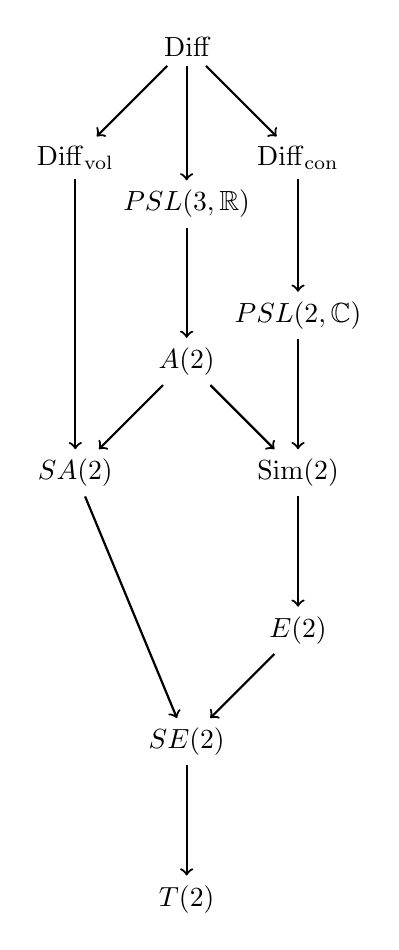
\begin{tikzpicture}[node distance=2cm]
\node(C1) [] {Diff};
\node(C2) [below left of=C1] {$\mathrm{Diff}_{\mathrm{vol}}$};
\node(C3) [below right of=C1] {$\mathrm{Diff}_{\mathrm{con}}$};
\node(B1)    [below of=C1]    {$PSL(3,\mathbb{R})$};
\node(A1) [below of=C3]                          {$PSL(2,\mathbb{C})$};
\node(B2)   [below of=B1]              {$A(2)$};
\node(A2)       [below right of=B2]          {Sim$(2)$};
%\node(A3)      [right of=A2]              {$PSL(2,\mathbb{R})$};
\node(B3)   [below left of=B2]            {$SA(2)$};
\node(A4)      [below of=A2]            {$E(2)$};
\node(A6)      [below left of=A4]            {$SE(2)$};
\node(A5) [below of=A6]{$T(2)$};

\draw[thick,->] (C1) to  (C2);
\draw[thick,->] (C1) to  (C3);
\draw[thick,->] (C1) to  (B1);
\draw[thick,->] (C2) to  (B3);
%\draw[thick,->] (C1) to  (A2);
\draw[thick,->] (C3) to  (A1);
\draw[thick,->] (A1)   to (A2);
\draw[thick,->] (B1) to  (B2);
\draw[thick,->] (B2) to  (B3);
\draw[thick,->] (B2) to  (A2);
\draw[thick,->] (A2) to  (A4);
\draw[thick,->] (B3) to  (A6);
\draw[thick,->] (A4) to  (A6);
\draw[thick,->] (A6) to  (A5);
\end{tikzpicture}
\end{center}
\caption{The lattice of groups considered in this paper. The edges identify subgroups.}
\end{figure}

%Groups we've done:
%translations, E(2), Sim(2), SA(2), A(2), PSL(2,C), PSL(3,R), Diff\_con, Diff\_vol, Diff

We consider as our image, the following function, defined on $[-1, 1]
\times:
[-1, 1]$
\begin{equation}\label{eq:function}
  \begin{split}
    f(x, y) &= 0.5 - 0.2x - 0.3y - 0.05x^2 + 0.03xy + 0.04y^2 \\ 
    &+ 0.03y^3 + 0.001x^3 - 0.0015x^2y + 0.002xy^2 - 0.0005y^3.
  \end{split}
\end{equation}
This function was chosen to have no critical points, and to be
predominantly linear, so that the higher order derivatives were not too
large. This was predominantly so the higher order terms in the signatures
would not overwhelm the smaller terms. The function is depicted as a
greyscale image in Figure~\ref{fig:function}
\begin{figure}
  \centering
  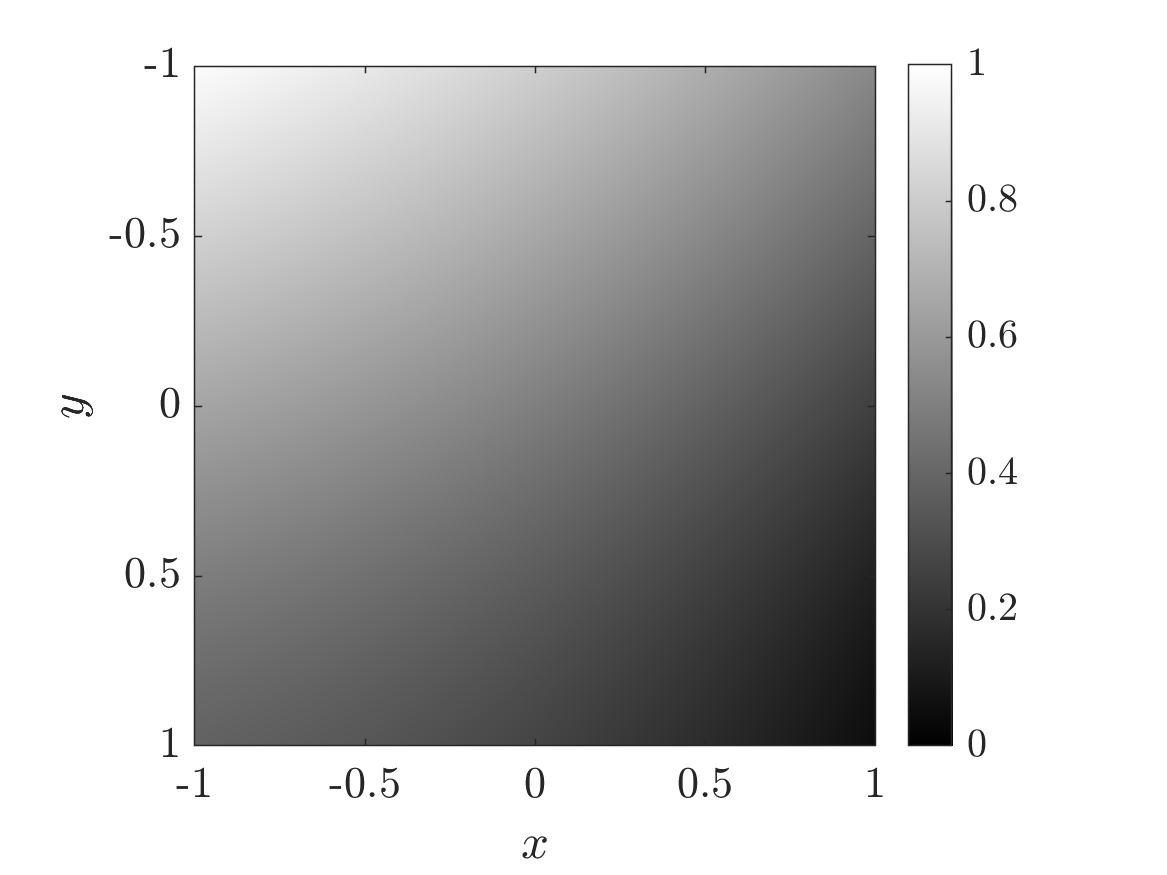
\includegraphics[width=12cm]{Figs/function}
  \caption{The test function used in this document, from
  Eq.~\eqref{eq:function}.}\label{fig:function}
\end{figure}

We consider the signatures of this function under various transformation
groups, as detailed throughout the main body of the paper and illustrate
the signature in three dimensions. A grid is overlaid on the image of the
function itself, as shown in Fig~\ref{fig:function_scanlines}. This grid is
mapped to the signature surface to help understand what the signature looks
like locally.
\begin{figure}
  \centering
  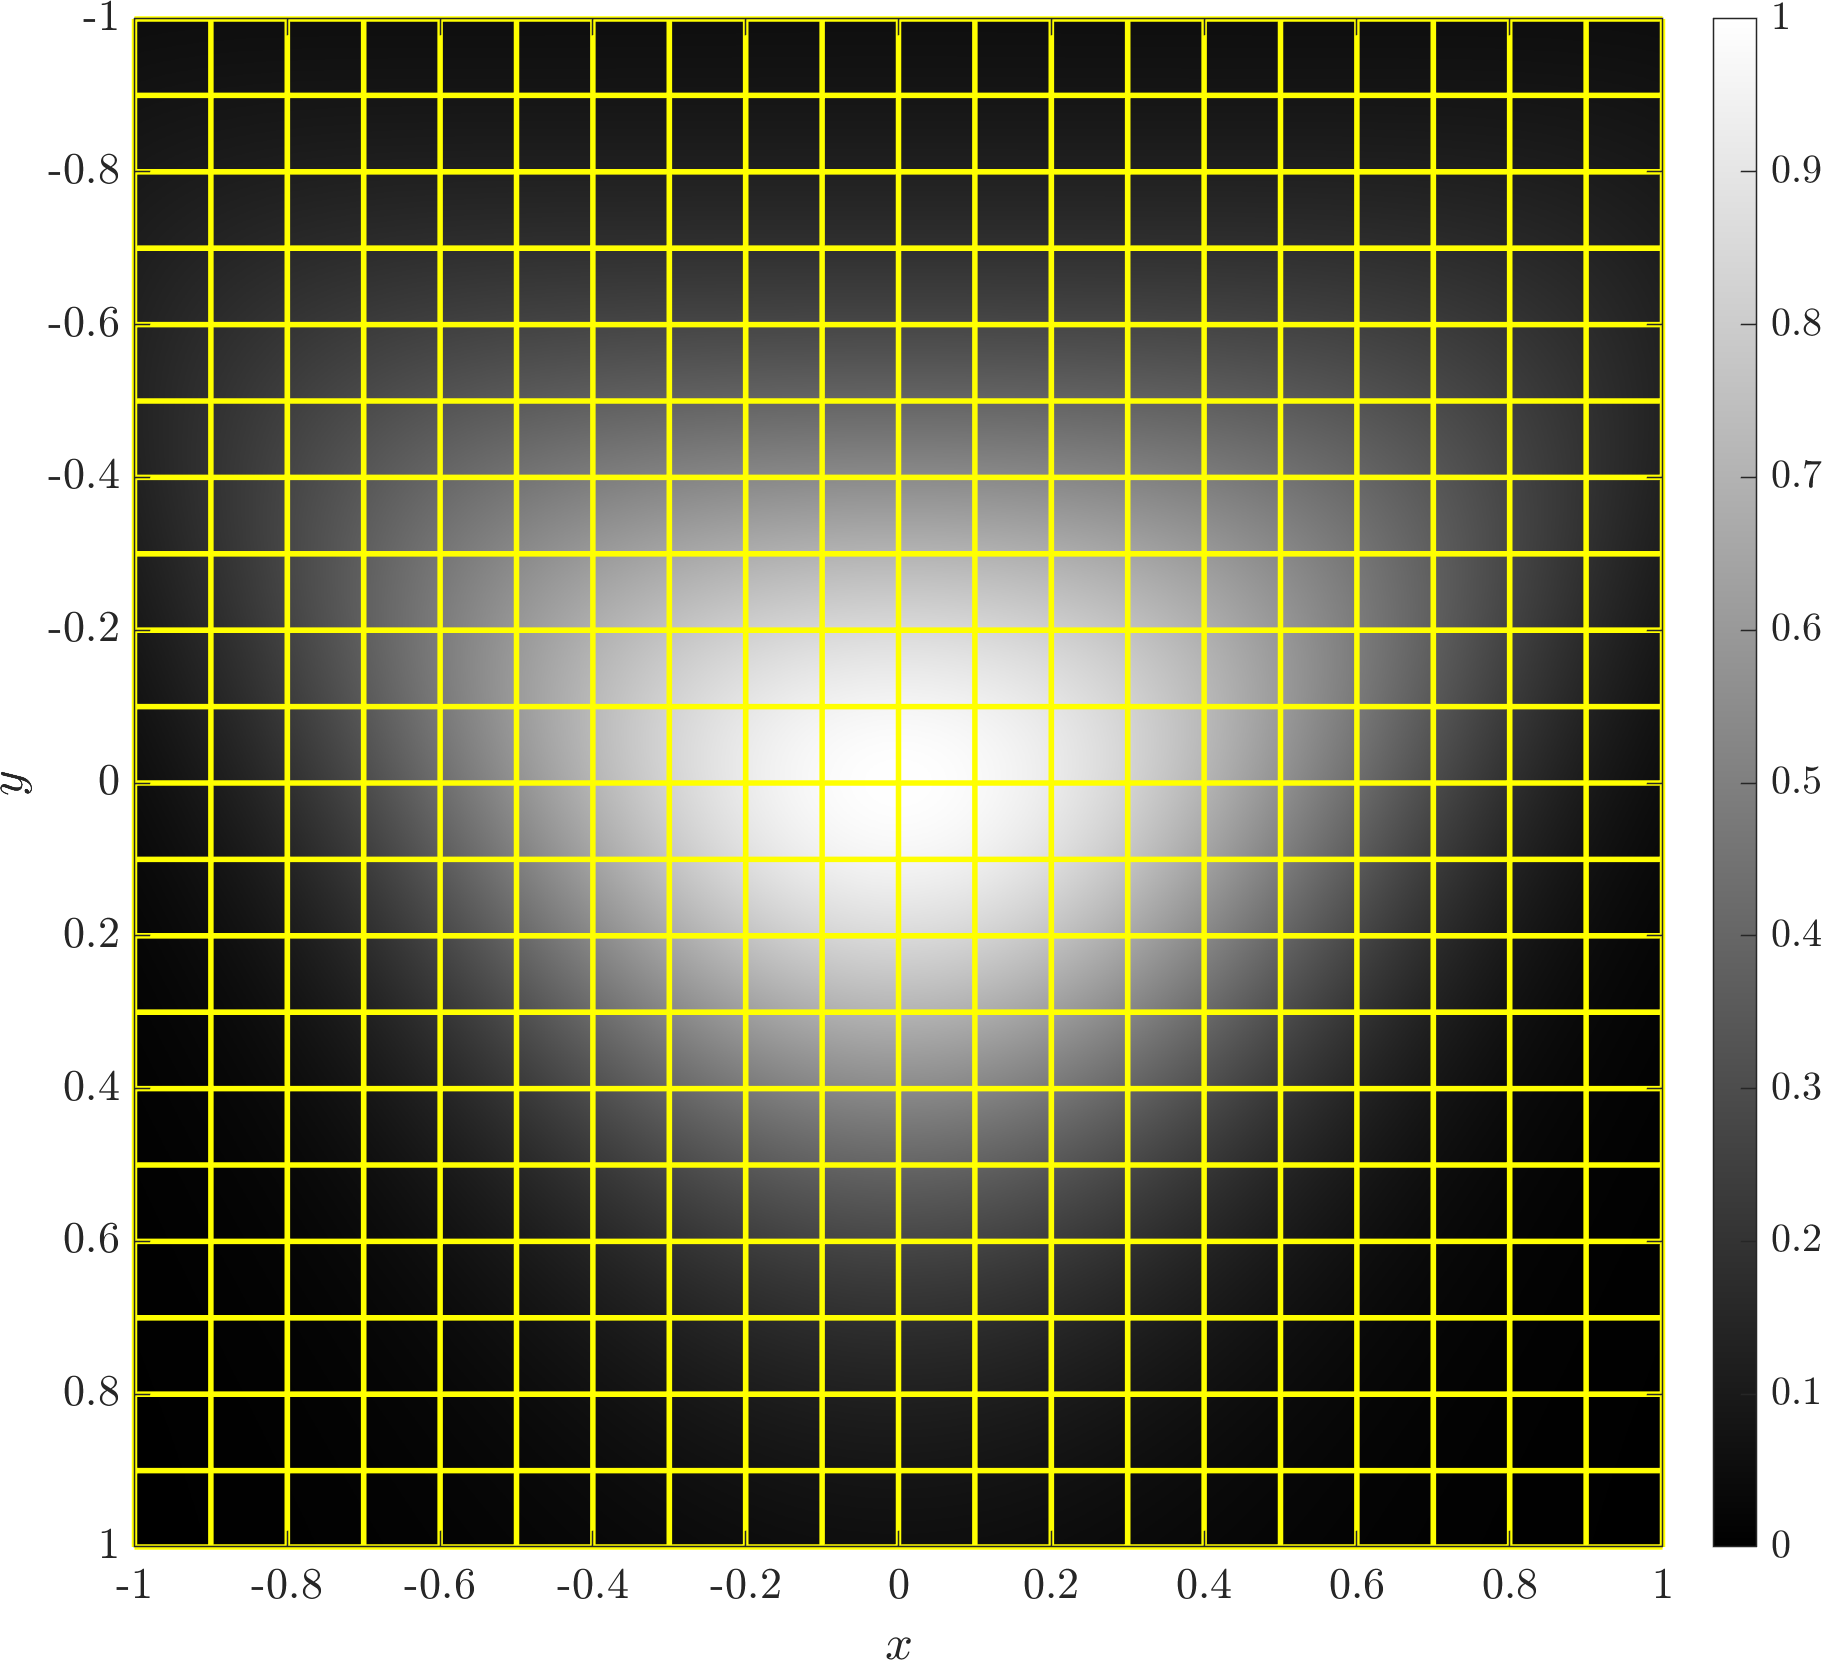
\includegraphics[width=12cm]{Figs/function_scanlines}
  \caption{The test function used in this document, from
  Eq.~\eqref{eq:function} with a grid of lines
overlaid.}\label{fig:function_scanlines}
\end{figure}

\section{Differential invariants through tensor contraction}
While we avoid the use of tensors in most of this study, there is a notable exception to be made for the Euclidean transformation group $E(2)$. In this setting we can restrict ourselves to \emph{Cartesian tensors}, where we need make no distinction between covariance and contravariance as they are equivalent. We therefore use subscript indices exclusively.

In this setting, a Euclidean transformation acting on $\mathbb{R}^2$ is given
by an expression of the form:
\begin{equation*}
  \bar{x}_i = a_{ij}x_j + b_j,
\end{equation*}
using the Einstein summation convention. The orthogonality condition is that $a_{ik}a_{jk} = a_{ki}a_{kj} = \delta_{ij}$.

With respect to $\mathbb{R}^2$, a Cartesian tensor of rank $p$, or $p$-tensor is a $2^p$-tuple of real numbers $C_{i_1\ldots i_p}$ whose components transform under a Euclidean transformation as:
\begin{equation*}
  \bar{C}_{i_1\ldots i_p} = a_{i_1j_1}\cdots a_{i_pj_p} C_{j_1\ldots j_p}
\end{equation*}
and a $0$-tensor is a scalar, or invariant. 

The main observation is that in this setting, the $n^\text{th}$ order partial derivative operator $\partial^n / \partial_{x_{i_1}}\cdots \partial_{x_{i_n}}$ formally transforms as an $n$-tensor. \todo[inline]{Cite Florack et al, 1993} Because the product of a $p$-tensor and a $q$-tensor gives a $(p+q)$-tensor and contraction of a $p$-tensor yields a $(p-2)$-tensor, a complete contraction of a tensor of even rank formed as a product of terms of the form $\partial^p f / \partial_{x_{i_1}} \cdots \partial_{x_{i_p}}$ will give a Euclidean invariant.

For example, up to second derivatives, we have the following Euclidean invariants, expressed as tensor contractions:
\begin{align*}
  f &= f \\
  f_if_i &= f_x^2 + f_y^2 \\
  f_{ii} &= f_{xx} + f_{yy} \\
  f_{ij} f_{ij} &= f_{xx}^2 + 2f_{xy}^2 + f_{yy}^2 \\
  f_i f_j f_{ij} &= f_x^2 f_{xx} + 2f_x f_y f_{xy} + f_y^2 f_{yy}
\label{eq:se2}
\end{align*}

While we can construct any number of invariants this way, there is no guarantee of functional independence of the constructed invariants. We will address this issue in Section~\ref{sec:movingframes} when we construct invariants of $E(2)$ and other groups using the method of moving frames.

\todo[inline]{Expand to Sim(2)}
\todo[inline]{Introduce image that we are going to use in subsequent examples}
\todo[inline]{Introduce signatures - 3D and 4D perhaps?}

\section{Differential invariants through transvectants}

Another way to compute invariants is to compare the action of group elements on separate copies of the underlying space (here, $\mathbb{R}^2$).

We will demonstrate this for the affine group $A(2)$ and its subgroup
$SA(2)$ where, following the treatment in~\cite{OlverCIT}, this leads to
Cayley's Omega Process~\cite{Cayley1846}. 

Consider $\mathbf{x}_i \in \mathbb{R}^2, i=1,2$, so that $\mathbf{x}_i$ can
be written in coordinates as $(x_i, y_i)$. Then a pair of such $\mathbf{x}$ lie in $\mathbb{R}^2 \times \mathbb{R}^2$. Now consider applying the same affine transformation to each $\mathbf{x}$ independently: $\mathbf{x}_i \mapsto A \mathbf{x}_i + \mathbf{b}$ where $A \in GL(2,\mathbb{R}$) and $\mathbf{b} \in \mathbb{R}^2$. Then the Omega Process is a second-order differential operator defined by: 
\begin{equation}
\Omega_{ij} = \begin{vmatrix} \frac{\partial}{\partial x_i} &
\frac{\partial}{\partial y_i} \\ \frac{\partial}{\partial x_j} &
\frac{\partial}{\partial y_j} \end{vmatrix} = 
\frac{\partial^2}{\partial x_i
\partial y_j} - \frac{\partial^2}{\partial x_j \partial y_i}.
\end{equation}

Under the above affine transformation, $\Omega_{ij} \mapsto (\det A)^{-1}
\Omega_{ij}$. Note that $(\det A)^{-1}$ has no dependence on the coordinates.
The Omega Process can be applied to pairs of smooth functions as follows,
writing $\frac{\partial f}{\partial x}$ as $f_x$:

\begin{equation}
\Omega_{ij} \left(f(x_i, y_i) g(x_j, y_j)\right) = f_{x_i}g_{y_j} - f_{y_i}g_{x_j}.
\end{equation}

Identifying $x_i = x_j = x, y_i = y_j = y$ gives us functions of $x$ and $y$
that only vary by a scaling factor of $(\det A)^{-1}$ when $\mathbf{x}$ is
mapped by an affine transformation. This matches the definition of a
first-order partial transvectant of two functions:

\begin{equation}
\mbox{tr} \Omega_{ij} f(x_i, y_i) g(x_j, y_j),
\end{equation}

\noindent where $\mbox{tr}$  is the operator that identifies the coordinates of each function $x_i = x_j = x, y_i = y_j = y$.

This can be generalised to $n$ functions $f^{(1)}(x_1, y_1), \ldots, f^{(n)}(x_n, y_n)$ and $r$-th order~\cite{OlverEIS} to define a partial transvectant as:

\begin{equation}
\mbox{tr} \left[\left( \Pi_{k=1}^r \Omega_{i_k j_k} \right) f^{(1)}(x_1, y_1)
f^{(2)}(x_2, y_2), \ldots f^{(n)} (x_n, y_n)\right],
\end{equation}
where $i_k \neq j_k \in \{1, \ldots, n\}$.

Under this formula we end with a factor $(\det A)^{-r}$ in place of $(\det
A)^{-1}$ that we saw previously, when all $n$ copies of $\mathbb{R}^2$ are
transformed by the same affine function $\mathbf{x} \mapsto A\mathbf{x} +
\mathbf{b}$. $r$ is referred to as the weight of the partial
transvectant. It can also be useful to consider the maximum order of
derivative in the transvectant, which we term degree, e.g., $f_{xy}^2 f_x
f_y$ has degree 2. Note also that the individual pairwise Omega processes commute.

For the current case it is sufficient to consider $n$ copies of the same
function $f$. If we represent each copy (of $\mathbb{R}^2$) as a node on a
undirected graph, and each Omega process $\Omega_{ij}$ as an edge joining
nodes $i$ and $j$, a partial transvectant can be compactly represented in a
graphical form. 

For example, consider a weight $2$ transvectant defined as:
\begin{align*}
    \mbox{tr} &\left[(\Omega_{12}\Omega_{12}) f(x_1, y_1)f(x_2, y_2)\right] \\
    &= \mbox{tr}\left[(\partial_{x_1 y_2} - \partial_{x_2y_1})(\partial_{x_1 y_2} -
    \partial_{x_2y_1})f(x_1, y_1)f(x_2, y_2)\right]\\
    &= \mbox{tr}\left[\left(\partial_{x_1 y_2} - \partial_{x_2 y_1}\right)\left(f_x(x_1, y_1)f_y(x_2, y_2) - f_y(x_1, y_1)f_x(x_2, y_2)\right)\right] \\
    &= \mbox{tr}\left[f_{xx}(x_1, y_1)f_{yy}(x_2, y_2) - f_{xy}(x_1, y_1)f_{xy}(x_2, y_2)\right] \\
    &= f_{xx}(x, y) f_{yy}(x, y) - f_{xy}(x, y)^2.
\end{align*}
This is a degree $2$ partial transvectant as it involves derivatives of $f$
up to second-order, and can be represented graphically by the following
diagram:
\begin{center}
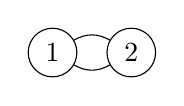
\begin{tikzpicture}[baseline=0]
    \node[draw,circle,minimum size=0.2cm] (1) at (-0.5,0) {1};
    \node[draw,circle,minimum size=0.2cm] (2) at (0.5,0) {2};
    \draw[-] (1) to [out=30,in=150] (2);
    \draw[-] (1) to [out=-30,in=-150] (2);
\end{tikzpicture}
\end{center}
where the double edge between nodes $1$ and $2$ corresponds to the two copies of $\Omega_{12}$.
Tables~\ref{tab:transvectants1} and~\ref{tab:transvectants2} shows all possible nonzero partial
transvectants of $A_2$ up to weight $4$ that can be generated in this way.
Note that the weight is the number of edges in the graph.

\begin{table}
\centering
\begin{tabular}{cccp{11cm}}
Degree & Weight & Diagram & Partial transvectant\\
\hline
2 & 2 &
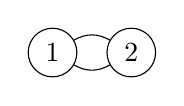
\begin{tikzpicture}[baseline=0]
    \node[draw,circle,minimum size=0.2cm] (1) at (-0.5,0) {1};
    \node[draw,circle,minimum size=0.2cm] (2) at (0.5,0) {2};
    \draw[-] (1) to [out=30,in=150] (2);
    \draw[-] (1) to [out=-30,in=-150] (2);
\end{tikzpicture}
& $2 f_{xx} f_{yy} - 2 \left(f_{xy}\right)^{2}$ \\

2 & 2 &
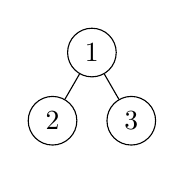
\begin{tikzpicture}[baseline=0]
    \node[draw,circle,minimum size=0.2cm] (1) at (0,0.866) {1};
    \node[draw,circle,minimum size=0.2cm] (2) at (-0.5,0) {2};
    \node[draw,circle,minimum size=0.2cm] (3) at (0.5,0) {3};
    \draw[-] (1) to (2);
    \draw[-] (1) to (3);
\end{tikzpicture}
& $\left(f_{x}\right)^{2} f_{yy} - 2 f_{x} f_{y} f_{xy} + f_{xx}
\left(f_{y}\right)^{2}$ \\

2 & 4 &
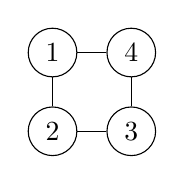
\begin{tikzpicture}[baseline=0]
    \node[draw,circle,minimum size=0.2cm] (1) at (0,1) {1};
    \node[draw,circle,minimum size=0.2cm] (2) at (0,0) {2};
    \node[draw,circle,minimum size=0.2cm] (3) at (1,0) {3};
    \node[draw,circle,minimum size=0.2cm] (4) at (1,1) {4};
    \draw[-] (1) to (2);
    \draw[-] (2) to (3);
    \draw[-] (3) to (4);
    \draw[-] (4) to (1);
\end{tikzpicture}
& $2 \left(f_{xx}\right)^{2} \left(f_{yy}\right)^{2} - 4 f_{xx} f_{yy} \left(f_{xy}\right)^{2} + 2 \left(f_{xy}\right)^{4}$ \\

2 & 4 &
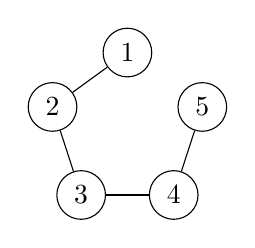
\begin{tikzpicture}[baseline=0]
    \node[draw,circle,minimum size=0.2cm] (1) at (0,1) {1};
    \node[draw,circle,minimum size=0.2cm] (2) at (-0.9511,0.3090) {2};
    \node[draw,circle,minimum size=0.2cm] (3) at (-0.5878,-.8090) {3};
    \node[draw,circle,minimum size=0.2cm] (4) at (0.5878,-.8090) {4};
    \node[draw,circle,minimum size=0.2cm] (5) at (0.9511,0.3090) {5};
    \draw[-] (1) to (2);
    \draw[-] (2) to (3);
    \draw[-] (3) to (4);
    \draw[-] (4) to (5);
\end{tikzpicture}
& $\left(f_{x}\right)^{2} f_{xx} \left(f_{yy}\right)^{2} - \left(f_{x}\right)^{2} f_{yy} \left(f_{xy}\right)^{2} - 2 f_{x} f_{xx} f_{y} f_{yy} f_{xy} + 2 f_{x} f_{y} \left(f_{xy}\right)^{3} + \left(f_{xx}\right)^{2} \left(f_{y}\right)^{2} f_{yy} - f_{xx} \left(f_{y}\right)^{2} \left(f_{xy}\right)^{2}$ \\

3 & 3 &
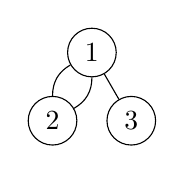
\begin{tikzpicture}[baseline=0]
    \node[draw,circle,minimum size=0.2cm] (1) at (0,0.866) {1};
    \node[draw,circle,minimum size=0.2cm] (2) at (-0.5,0) {2};
    \node[draw,circle,minimum size=0.2cm] (3) at (0.5,0) {3};
    \draw[-] (1) to [out=-150,in=90] (2);
    \draw[-] (1) to [out=-90,in=30] (2);
    \draw[-] (1) to (3);
\end{tikzpicture}
& $- f_{x} f_{xx} f_{yyy} - f_{x} f_{yy} f_{xxy} + 2 f_{x} f_{xy} f_{xyy} +
f_{xx} f_{y} f_{xyy} + f_{xxx} f_{y} f_{yy} - 2 f_{y} f_{xy} f_{xxy}$ \\

3 & 3 &
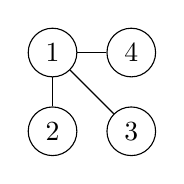
\begin{tikzpicture}[baseline=0]
    \node[draw,circle,minimum size=0.2cm] (1) at (0,1) {1};
    \node[draw,circle,minimum size=0.2cm] (2) at (0,0) {2};
    \node[draw,circle,minimum size=0.2cm] (3) at (1,0) {3};
    \node[draw,circle,minimum size=0.2cm] (4) at (1,1) {4};
    \draw[-] (1) to (2);
    \draw[-] (1) to (3);
    \draw[-] (1) to (4);
\end{tikzpicture}
& $- \left(f_{x}\right)^{3} f_{yyy} + 3 \left(f_{x}\right)^{2} f_{y} f_{xyy} - 3 f_{x} \left(f_{y}\right)^{2} f_{xxy} + f_{xxx} \left(f_{y}\right)^{3}$  \\

3 & 4 &
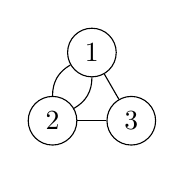
\begin{tikzpicture}[baseline=0]
    \node[draw,circle,minimum size=0.2cm] (1) at (0,0.866) {1};
    \node[draw,circle,minimum size=0.2cm] (2) at (-0.5,0) {2};
    \node[draw,circle,minimum size=0.2cm] (3) at (0.5,0) {3};
    \draw[-] (1) to [out=-150,in=90] (2);
    \draw[-] (1) to [out=-90,in=30] (2);
    \draw[-] (1) to (3);
    \draw[-] (2) to (3);
\end{tikzpicture}
& $2 f_{xx} f_{yyy} f_{xxy} - 2 f_{xx} \left(f_{xyy}\right)^{2} + 2 f_{xxx}
f_{yy} f_{xyy} - 2 f_{xxx} f_{yyy} f_{xy} - 2 f_{yy}
\left(f_{xxy}\right)^{2} + 2 f_{xy} f_{xyy} f_{xxy}$ \\


%=====

3 & 4 &
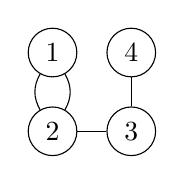
\begin{tikzpicture}[baseline=0]
    \node[draw,circle,minimum size=0.2cm] (1) at (0,1) {1};
    \node[draw,circle,minimum size=0.2cm] (2) at (0,0) {2};
    \node[draw,circle,minimum size=0.2cm] (3) at (1,0) {3};
    \node[draw,circle,minimum size=0.2cm] (4) at (1,1) {4};
    \draw[-] (1) to [out=-120,in=120] (2);
    \draw[-] (1) to [out=-60,in=60] (2);
    \draw[-] (2) to (3);
    \draw[-] (3) to (4);
\end{tikzpicture}
& $- f_{x} f_{xx} f_{yy} f_{xyy} + f_{x} f_{xx} f_{yyy} f_{xy} - f_{x} f_{xxx} \left(f_{yy}\right)^{2} + 3 f_{x} f_{yy} f_{xy} f_{xxy} - 2 f_{x} \left(f_{xy}\right)^{2} f_{xyy} - \left(f_{xx}\right)^{2} f_{y} f_{yyy} - f_{xx} f_{y} f_{yy} f_{xxy} + 3 f_{xx} f_{y} f_{xy} f_{xyy} + f_{xxx} f_{y} f_{yy} f_{xy} - 2 f_{y} \left(f_{xy}\right)^{2} f_{xxy}$ \\

3 & 4 &
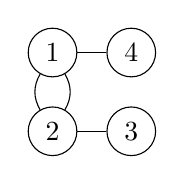
\begin{tikzpicture}[baseline=0]
    \node[draw,circle,minimum size=0.2cm] (1) at (0,1) {1};
    \node[draw,circle,minimum size=0.2cm] (2) at (0,0) {2};
    \node[draw,circle,minimum size=0.2cm] (3) at (1,0) {3};
    \node[draw,circle,minimum size=0.2cm] (4) at (1,1) {4};
    \draw[-] (1) to [out=-120,in=120] (2);
    \draw[-] (1) to [out=-60,in=60] (2);
    \draw[-] (2) to (3);
    \draw[-] (1) to (4);
\end{tikzpicture}
& $2 \left(f_{x}\right)^{2} f_{yyy} f_{xxy} - 2 \left(f_{x}\right)^{2} \left(f_{xyy}\right)^{2} - 2 f_{x} f_{xxx} f_{y} f_{yyy} + 2 f_{x} f_{y} f_{xyy} f_{xxy} + 2 f_{xxx} \left(f_{y}\right)^{2} f_{xyy} - 2 \left(f_{y}\right)^{2} \left(f_{xxy}\right)^{2}$ \\

% =========
3 & 4 &
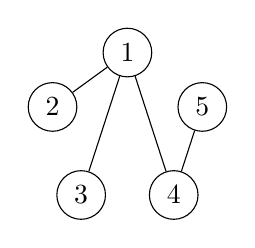
\begin{tikzpicture}[baseline=0]
    \node[draw,circle,minimum size=0.2cm] (1) at (0,1) {1};
    \node[draw,circle,minimum size=0.2cm] (2) at (-0.9511,0.3090) {2};
    \node[draw,circle,minimum size=0.2cm] (3) at (-0.5878,-.8090) {3};
    \node[draw,circle,minimum size=0.2cm] (4) at (0.5878,-.8090) {4};
    \node[draw,circle,minimum size=0.2cm] (5) at (0.9511,0.3090) {5};
    \draw[-] (1) to (2);
    \draw[-] (1) to (3);
    \draw[-] (1) to (4);
    \draw[-] (4) to (5);
\end{tikzpicture}
& $- \left(f_{x}\right)^{3} f_{yy} f_{xyy} + \left(f_{x}\right)^{3} f_{yyy} f_{xy} - \left(f_{x}\right)^{2} f_{xx} f_{y} f_{yyy} + 2 \left(f_{x}\right)^{2} f_{y} f_{yy} f_{xxy} - \left(f_{x}\right)^{2} f_{y} f_{xy} f_{xyy} + 2 f_{x} f_{xx} \left(f_{y}\right)^{2} f_{xyy} - f_{x} f_{xxx} \left(f_{y}\right)^{2} f_{yy} - f_{x} \left(f_{y}\right)^{2} f_{xy} f_{xxy} - f_{xx} \left(f_{y}\right)^{3} f_{xxy} + f_{xxx} \left(f_{y}\right)^{3} f_{xy}$ \\
\end{tabular}
\caption{Details and graphical representations of all partial transvectants up to degree $3$ of copies of a function $f$ under a transformation in $A(2)$.}
\label{tab:transvectants1}
\end{table}


\begin{table}
\centering
\begin{tabular}{cccp{11cm}}
Degree & Weight & Diagram & Partial transvectant\\
\hline
4 & 4 &
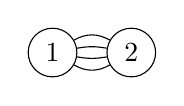
\begin{tikzpicture}[baseline=0]
    \node[draw,circle,minimum size=0.2cm] (1) at (-0.5,0) {1};
    \node[draw,circle,minimum size=0.2cm] (2) at (0.5,0) {2};
    \draw[-] (1) to [out=30,in=150] (2);
    \draw[-] (1) to [out=-30,in=-150] (2);
    \draw[-] (1) to [out=10,in=170] (2);
    \draw[-] (1) to [out=-10,in=-170] (2);
\end{tikzpicture}
& $f_{xxxx} f_{yyyy} - 4 f_{xyyy} f_{xxxy} + 3 f_{xxyy}^2$ \\


4 & 4 &
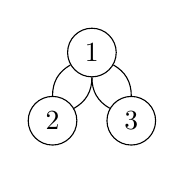
\begin{tikzpicture}[baseline=0]
    \node[draw,circle,minimum size=0.2cm] (1) at (0,0.866) {1};
    \node[draw,circle,minimum size=0.2cm] (2) at (-0.5,0) {2};
    \node[draw,circle,minimum size=0.2cm] (3) at (0.5,0) {3};
    \draw[-] (1) to [out=-150,in=90] (2);
    \draw[-] (1) to [out=-90,in=30] (2);
    \draw[-] (1) to [out=-90,in=150] (3);
    \draw[-] (1) to [out=-30,in=90] (3);
\end{tikzpicture}
& $ f_{xx}^2 f_{yyyy} + 2 f_{xx} f_{yy} f_{xxyy} - 4 f_{xx} f_{xy} f_{xyyy} - 4 f_{yy} f_{xy} f_{xxxy} + 4 f_{xy}^2 f_{xxyy} + f_{xxxx} f_{yy}^2$ \\


4 & 4 &
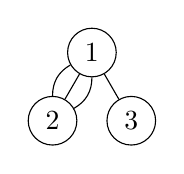
\begin{tikzpicture}[baseline=0]
    \node[draw,circle,minimum size=0.2cm] (1) at (0,0.866) {1};
    \node[draw,circle,minimum size=0.2cm] (2) at (-0.5,0) {2};
    \node[draw,circle,minimum size=0.2cm] (3) at (0.5,0) {3};
    \draw[-] (1) to [out=-150,in=90] (2);
    \draw[-] (1) to [out=-90,in=30] (2);
    \draw[-] (1) to (2);
    \draw[-] (1) to (3);
\end{tikzpicture} 
& $ f_{x} f_{xxx} f_{yyyy} - f_x f_{yyy} f_{xxxy} + 3 f_{x} f_{xyy} f_{xxyy} - 3 f_x f_{xyyy} f_{xxy} - f_{xxx} f_y f_{xyyy} + f_{xxxx} f_y f_{yyy} - 3 f_y f_{xyy} f_{xxxy} + 3 f_y f_{xxy} f_{xxyy}$ \\

4 & 4 &
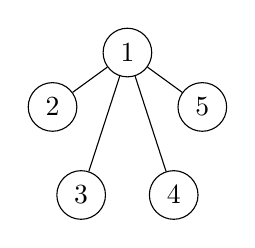
\begin{tikzpicture}[baseline=0]
    \node[draw,circle,minimum size=0.2cm] (1) at (0,1) {1};
    \node[draw,circle,minimum size=0.2cm] (2) at (-0.9511,0.3090) {2};
    \node[draw,circle,minimum size=0.2cm] (3) at (-0.5878,-.8090) {3};
    \node[draw,circle,minimum size=0.2cm] (4) at (0.5878,-.8090) {4};
    \node[draw,circle,minimum size=0.2cm] (5) at (0.9511,0.3090) {5};
    \draw[-] (1) to (2);
    \draw[-] (1) to (3);
    \draw[-] (1) to (4);
    \draw[-] (1) to (5);
\end{tikzpicture}
& $\left(f_{x}\right)^{4} f_{yyyy} - 4 \left(f_{x}\right)^{3} f_{y} f_{xyyy} + 6 \left(f_{x}\right)^{2} \left(f_{y}\right)^{2} f_{xxyy} - 4 f_{x} \left(f_{y}\right)^{3} f_{xxxy} + f_{xxxx} \left(f_{y}\right)^{4}$ \\
\end{tabular}
\caption{Details and graphical representations of all partial transvectants of weight $4$ of copies of a function $f$ under a transformation in $A(2)$.}
\label{tab:transvectants2}
\end{table}

\todo[inline]{Explain}

\subsection{Signatures of SA(2) and A(2)}
Recall that invariants of a supergroup are automatically invariants of any of
its subgroups. For example, invariants of $A(2)$ are automatically invariants of $SA(2)$, but not necessarily vice versa. Any of the partial transvectants found in Tables~\ref{tab:transvectants1} and~\ref{tab:transvectants2} are invariants of $SA(2)$ (as the determinant is $1$), but only up to scale factor ($\det A^{-r}$) of $A(2)$.

Hence, we can form a signature for $SA(2)$ by choosing any combination of
partial transvectants. We'll choose a signature with three components so that
it can be visualised as a three-dimensional surface; note that this will not
be complete and may well have a very large bad set. For example, we can choose the function value together with the first two partial transvectants to form the signature:
\begin{equation*}
    \left(f, f_{xx}f_{yy}-f_{xy}^2, f_x^2f_{yy} - 2f_xf_yf_{xy} + f_{xx}f_y^2\right).
\end{equation*}

\subsubsection{Example}
Consider as our image, the function $f(x, y) = 0.5 - 0.2x - 0.3y - 0.05x^2 +
0.03xy + 0.04y^2 + 0.03y^3 +0.001x^3 - 0.0015x^2y + 0.002xy^2 - 0.0005y^3$
defined on $[0, 1]\times[0, 1]$.
\todo[inline]{remake figure with modified matrix. Also modify function so it has some features like a critical point}
We'll subject our image to a special affine transformation:
\begin{equation*}
\mathbf{x} \mapsto \frac{1}{1.1}\begin{bmatrix} 0.6875 & 1.1 \\ -0.6 & 0.8 \end{bmatrix}\mathbf{x} + \begin{bmatrix} 0.1 \\ -0.2 \end{bmatrix}
\end{equation*}

Fig.~\ref{fig:SA2} shows the function as a greyscale image, the transformed
function, and the signatures of both the untransformed and transformed
images.
\begin{figure}
\centering
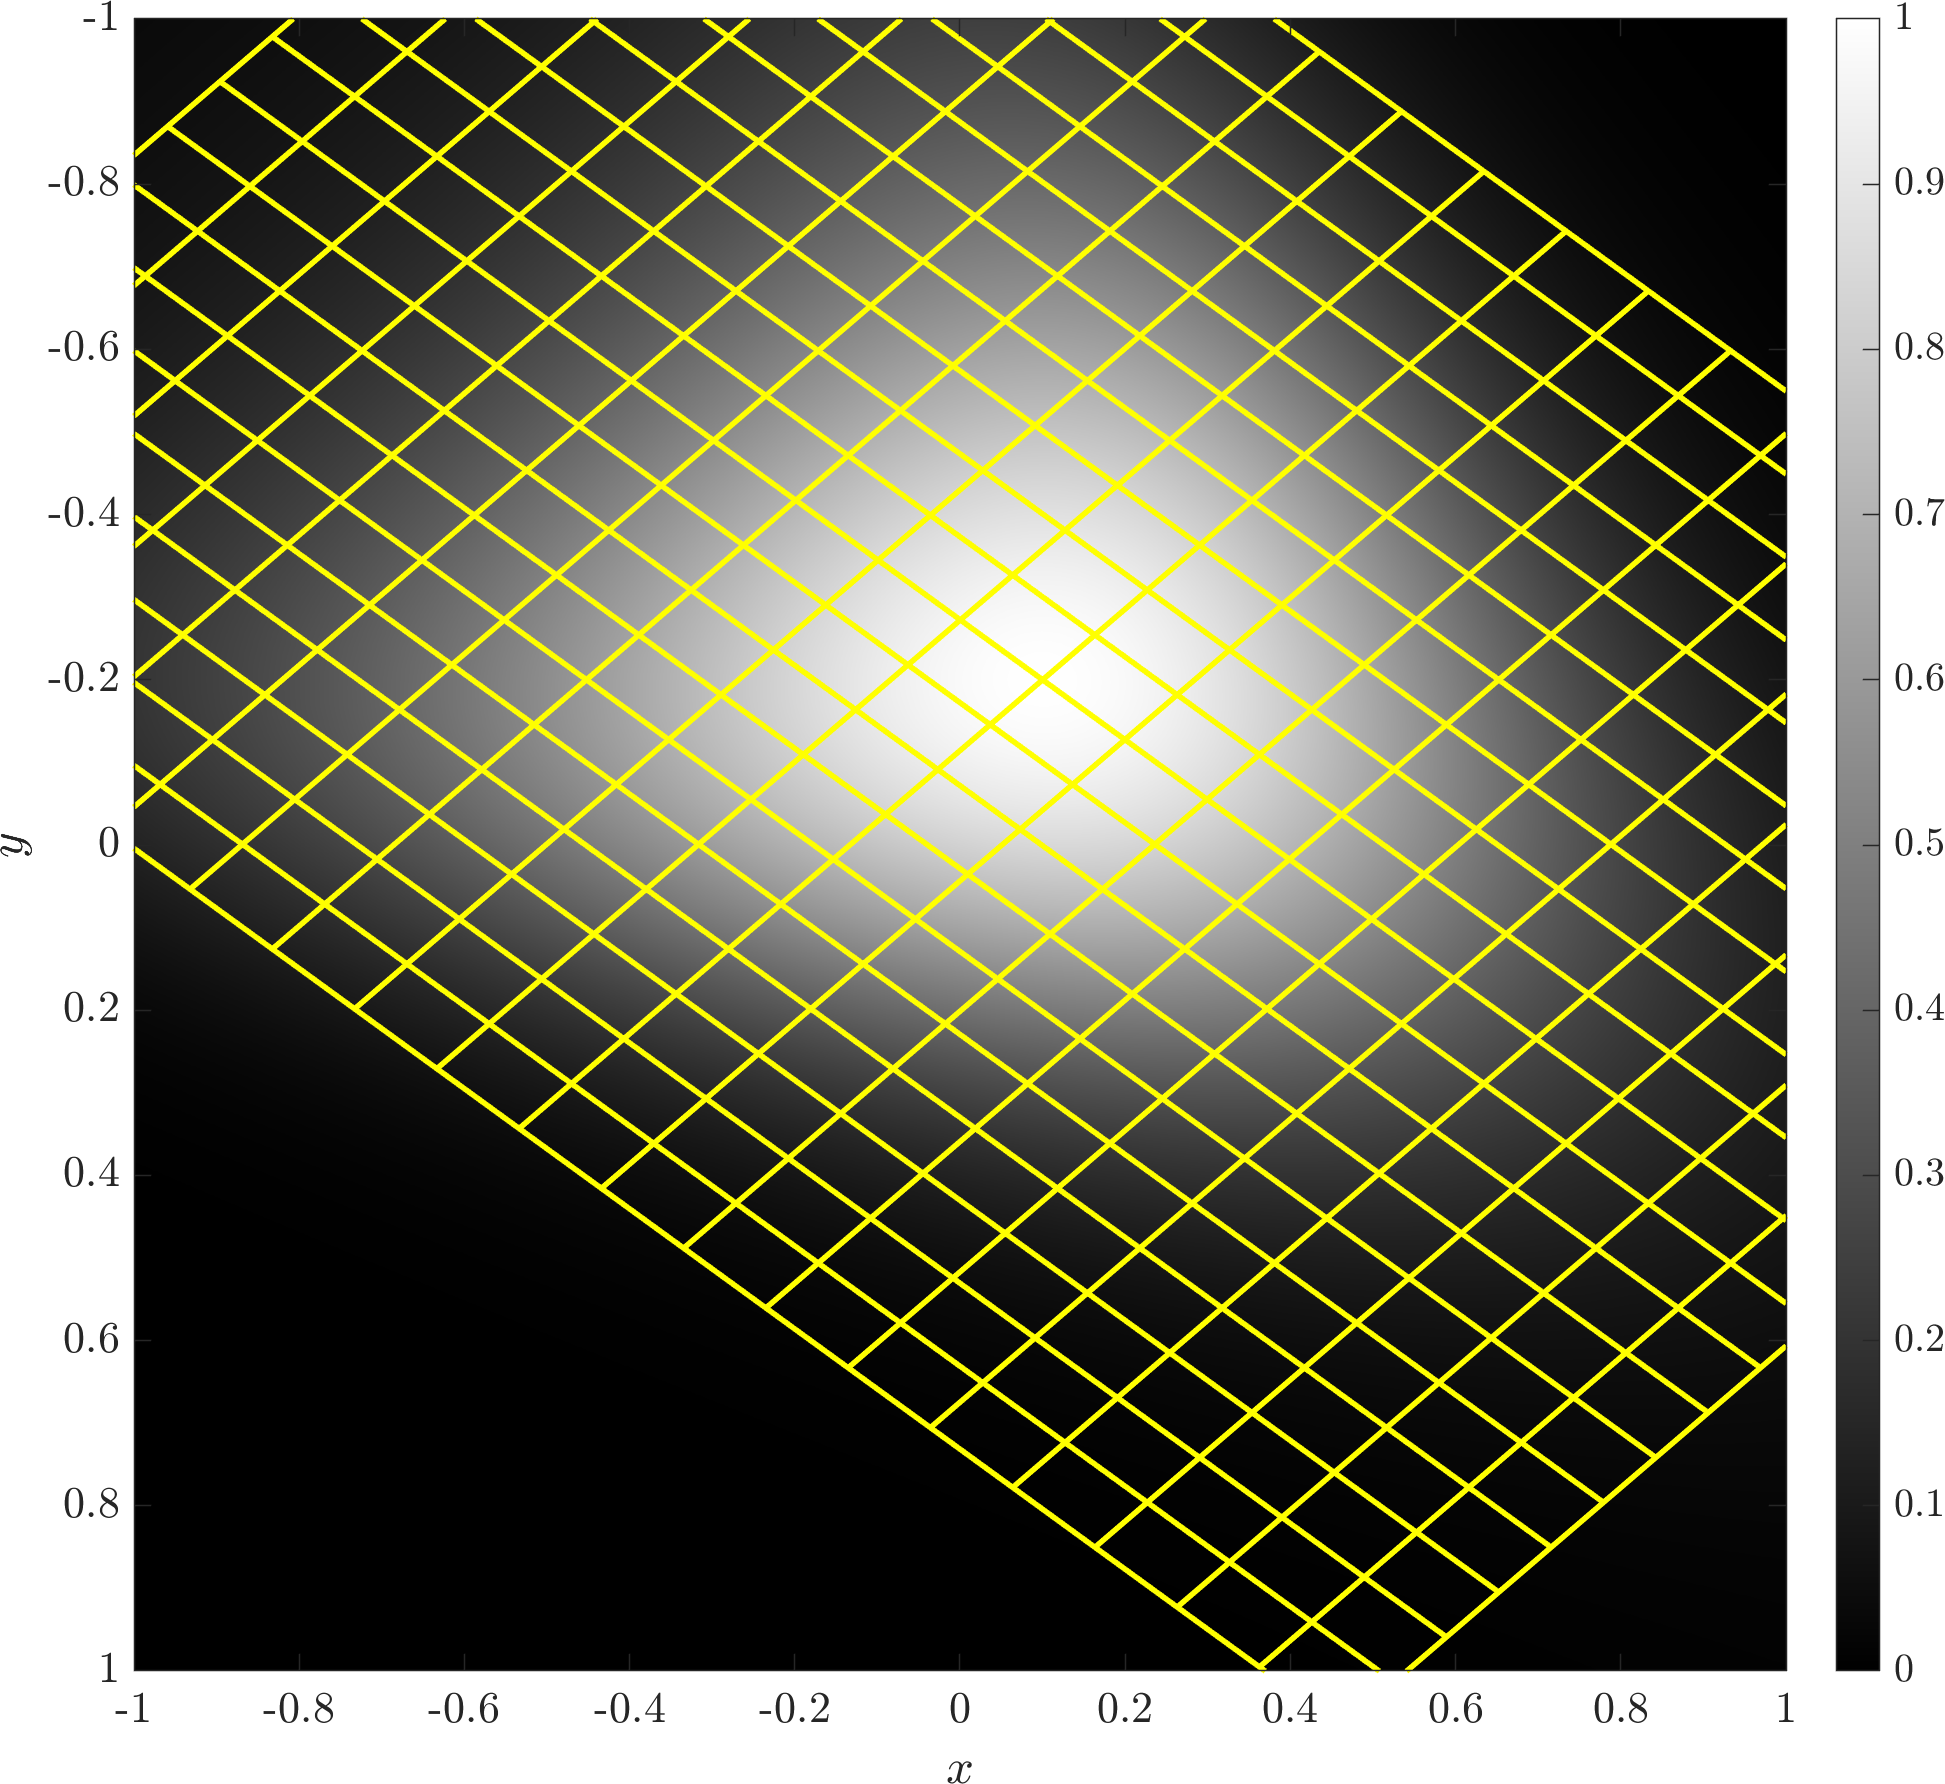
\includegraphics[width=.45\textwidth]{Figs/f_transformed_SA2.png}
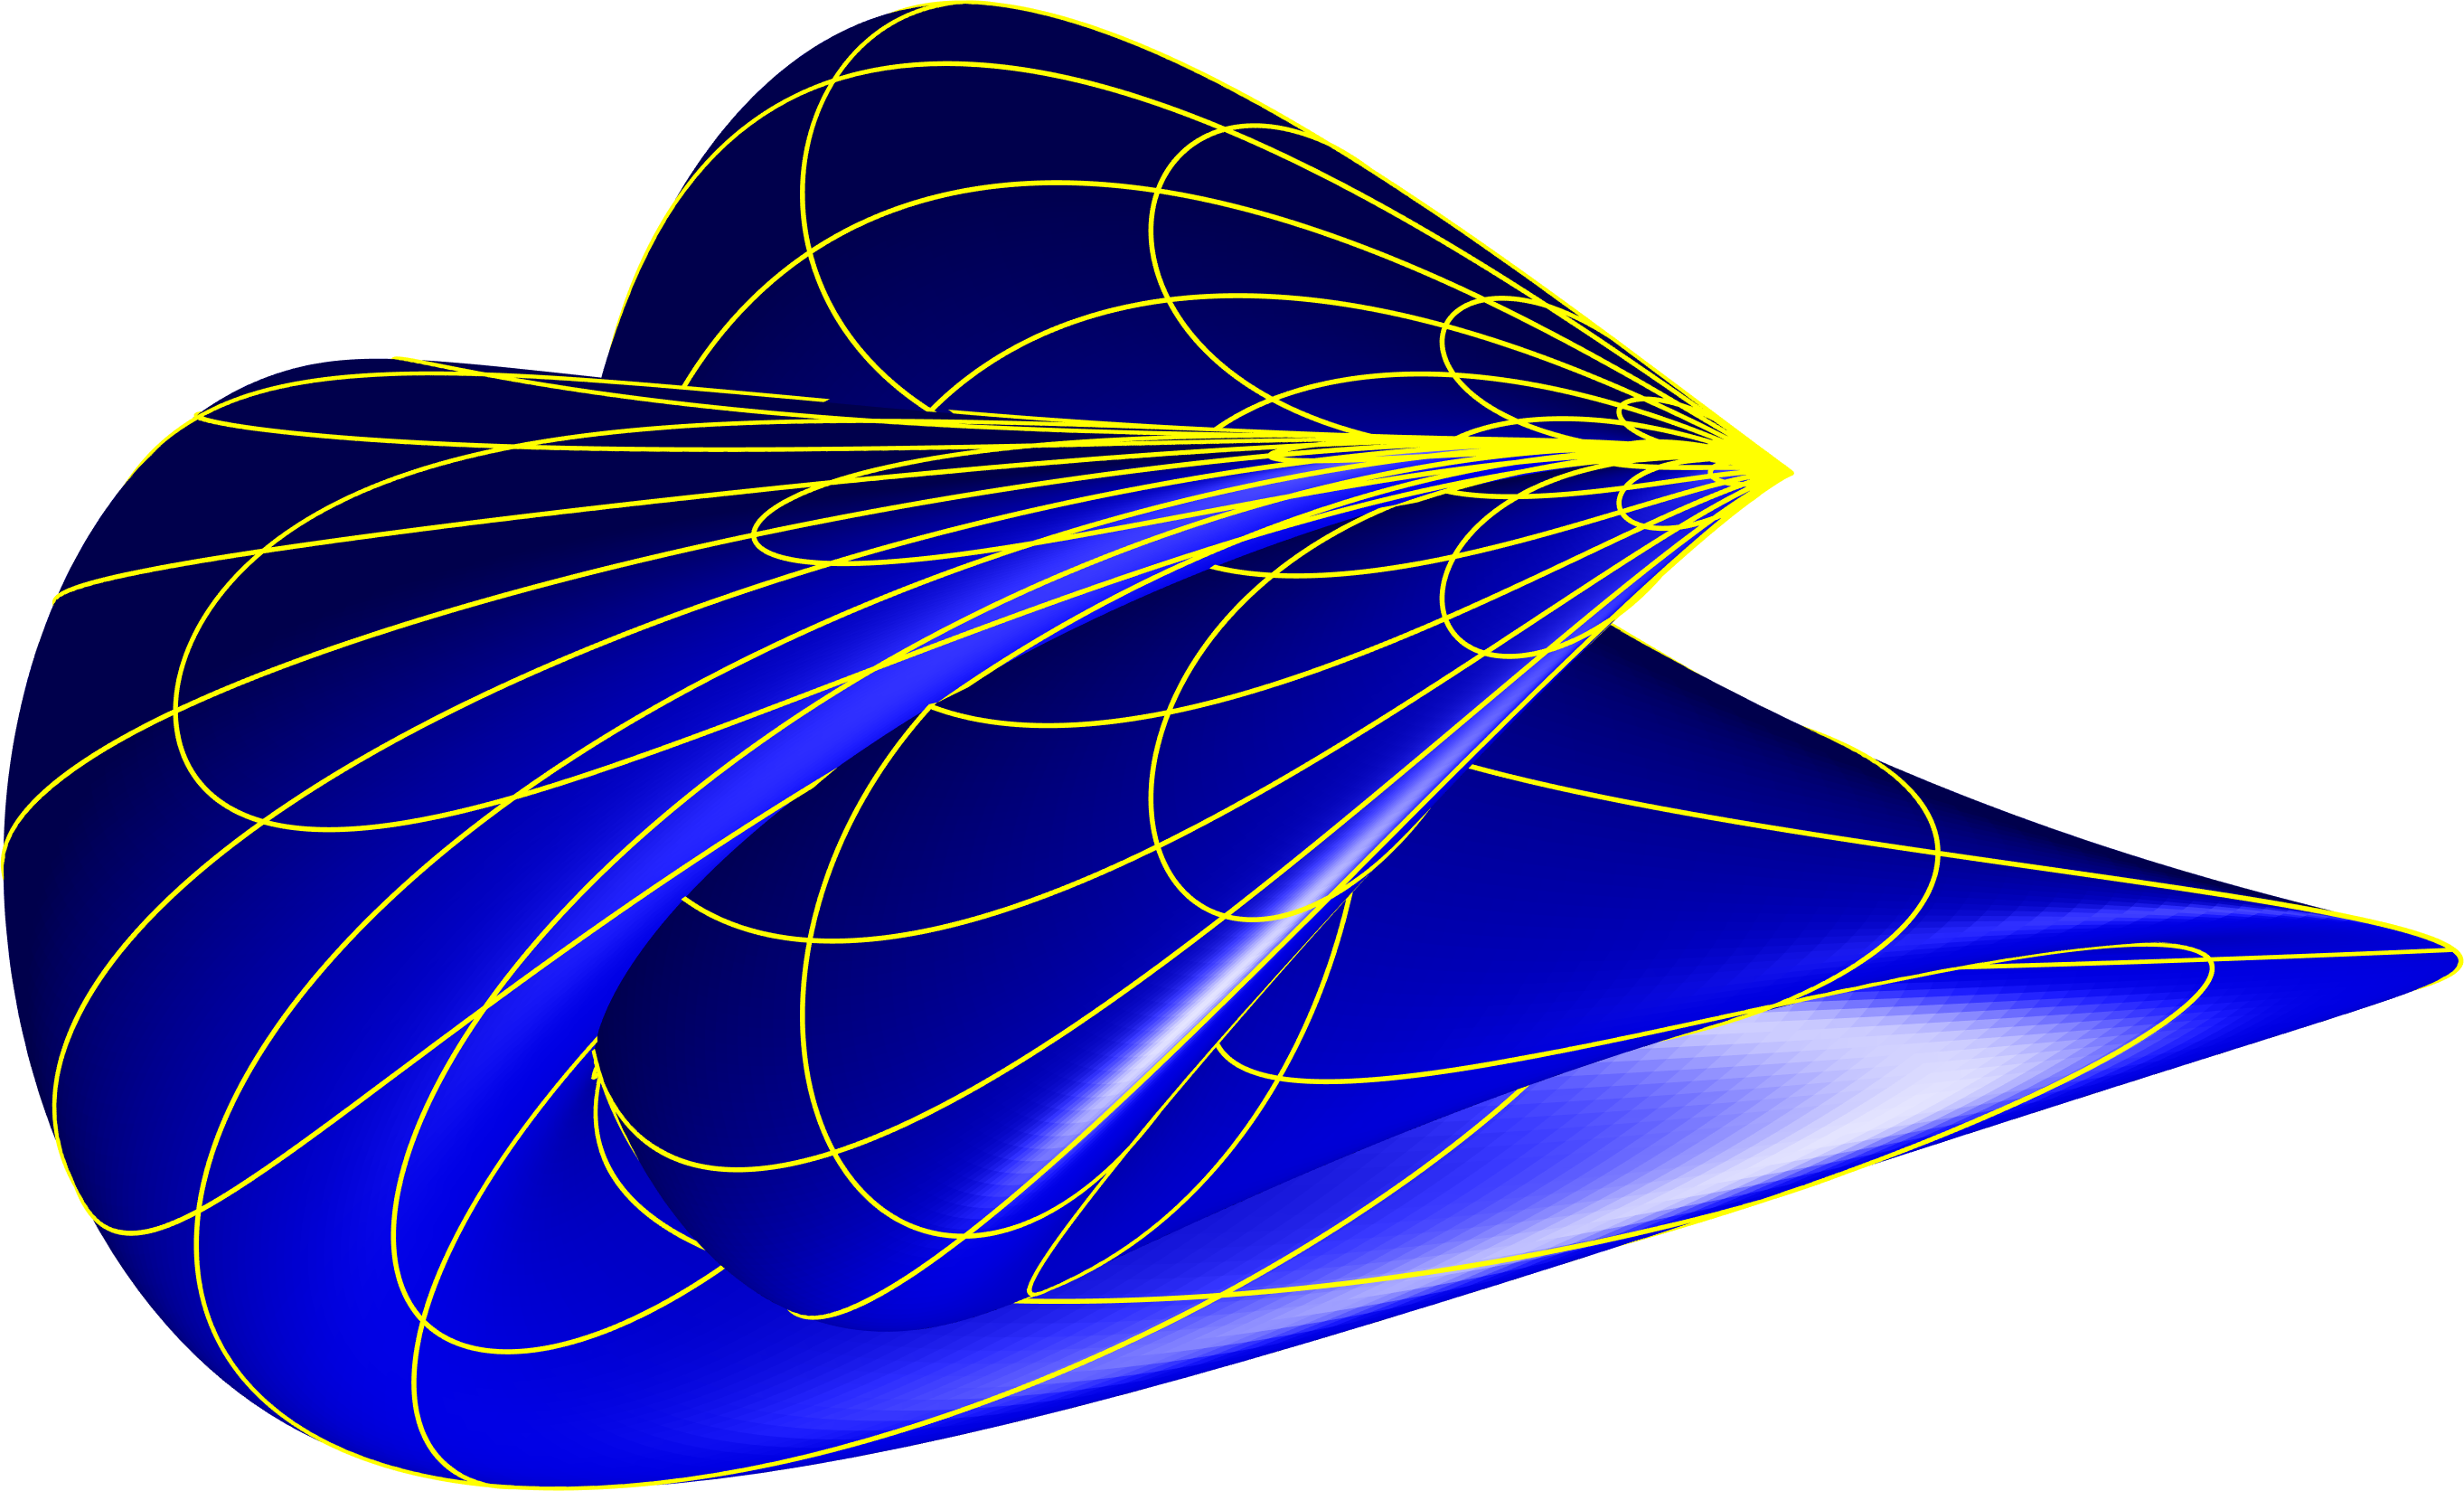
\includegraphics[width=.45\textwidth]{Figs/SA2_signature.png}
\caption{\todo[inline]{add extra crap} A sample $SA(2)$ Transform and 3D signature. Mention what's going on with the grid.}
\label{fig:SA2}
\end{figure}


\subsubsection{Moving on to A(2), \ldots}
Using the same function as an example, 
\begin{figure}
\centering
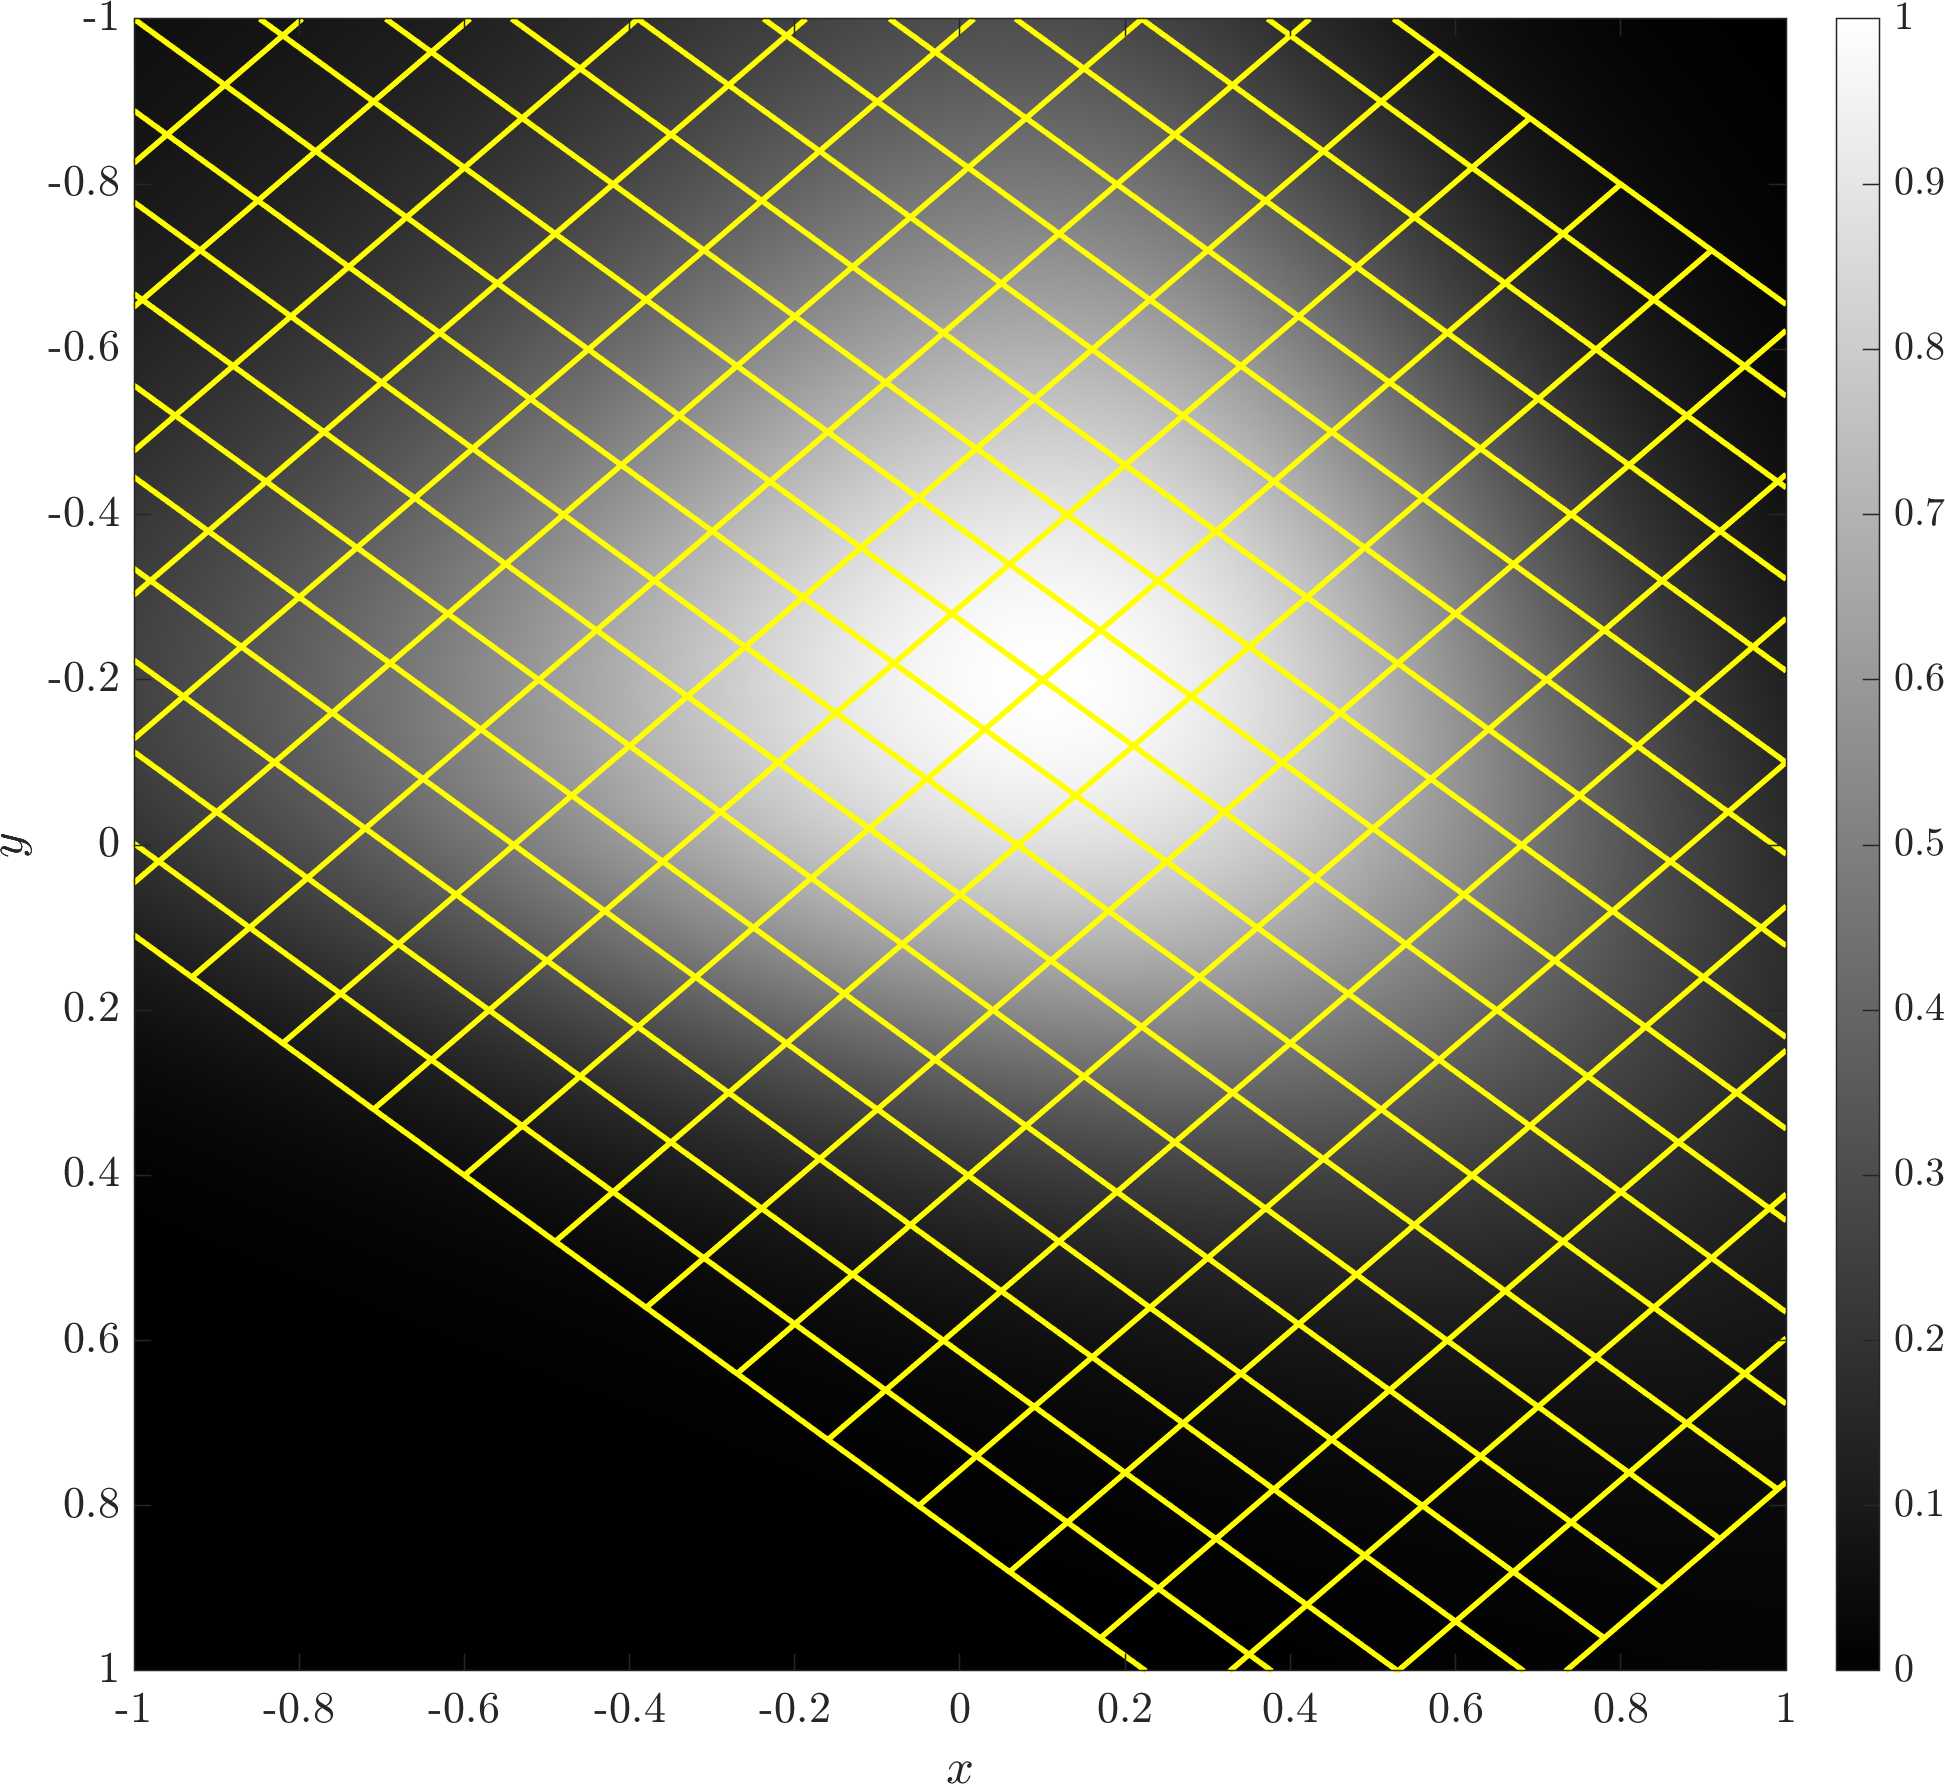
\includegraphics[width=.45\textwidth]{Figs/f_transformed_A2.png}
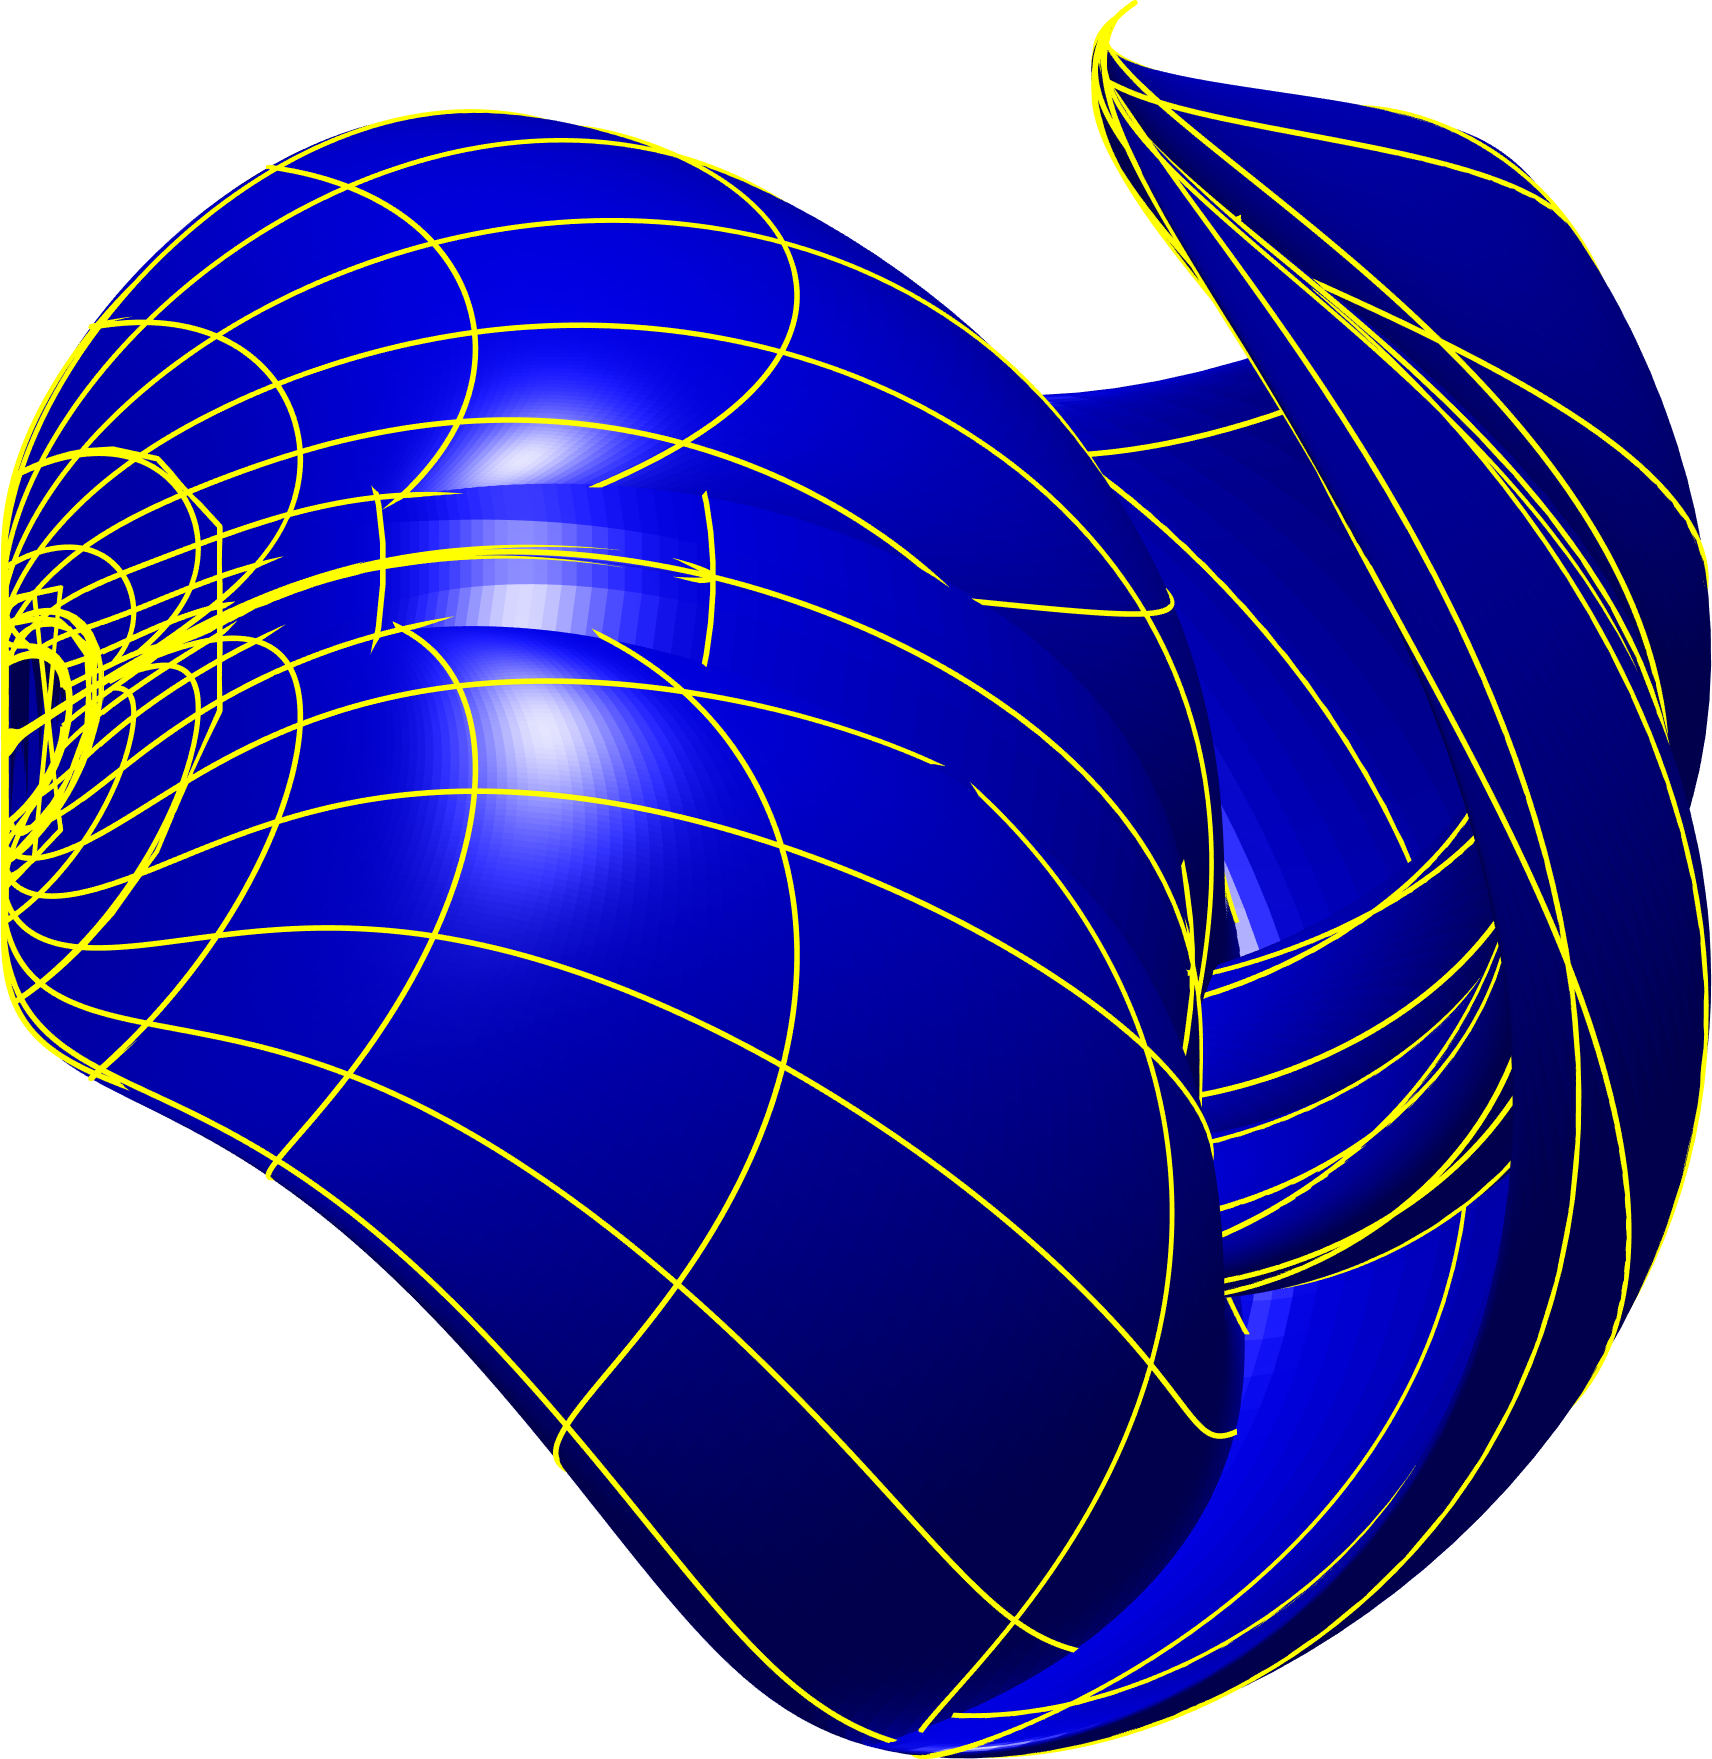
\includegraphics[width=.45\textwidth]{Figs/A2_signature.png}
\caption{A sample $A(2)$ Transform and 3D signature.}
\label{fig:A2}
\end{figure}

For $A(2)$ the weight of the partial transvectants prevents them from being invariants. They can be normalised by choosing only those where all components have the same weight and projecting them onto a unit hypersphere. Instead, we select ratios of partial transvectants. It is beneficial to choose the numerator and denominator so that they have different critical points, which can be achieved by adding together partial transvectants of the same weight as appropriate.

\begin{figure}
\centering
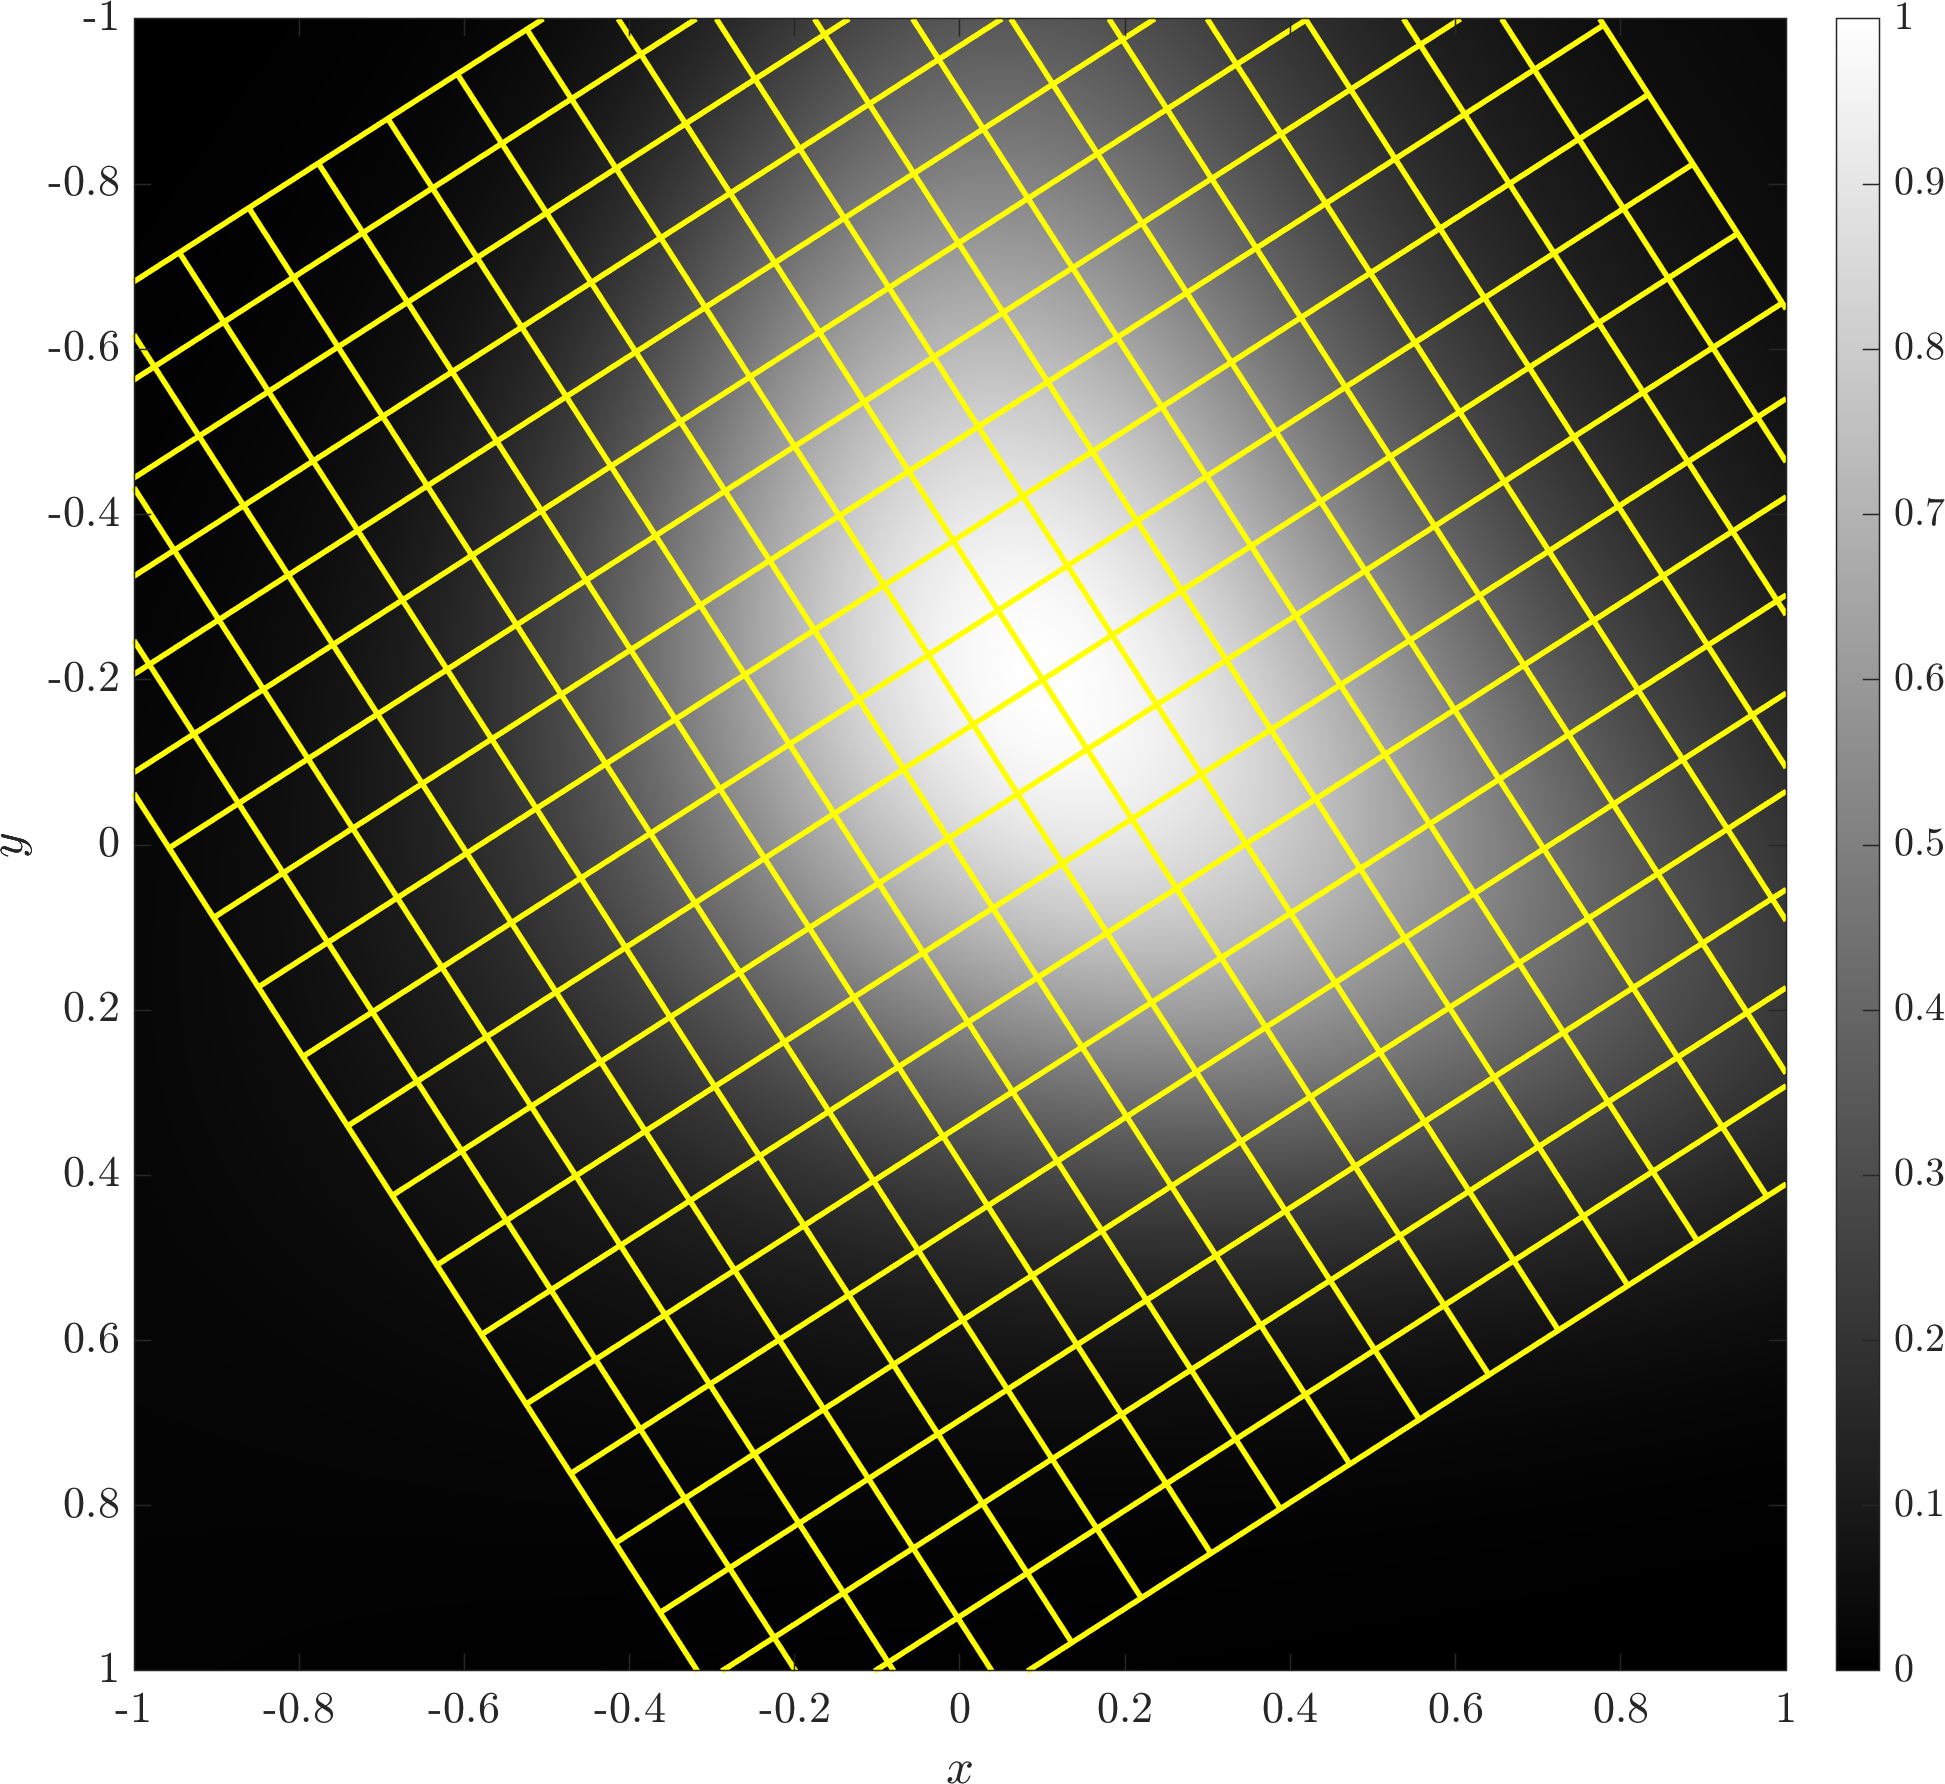
\includegraphics[width=.45\textwidth]{Figs/f_transformed_SE2.png}
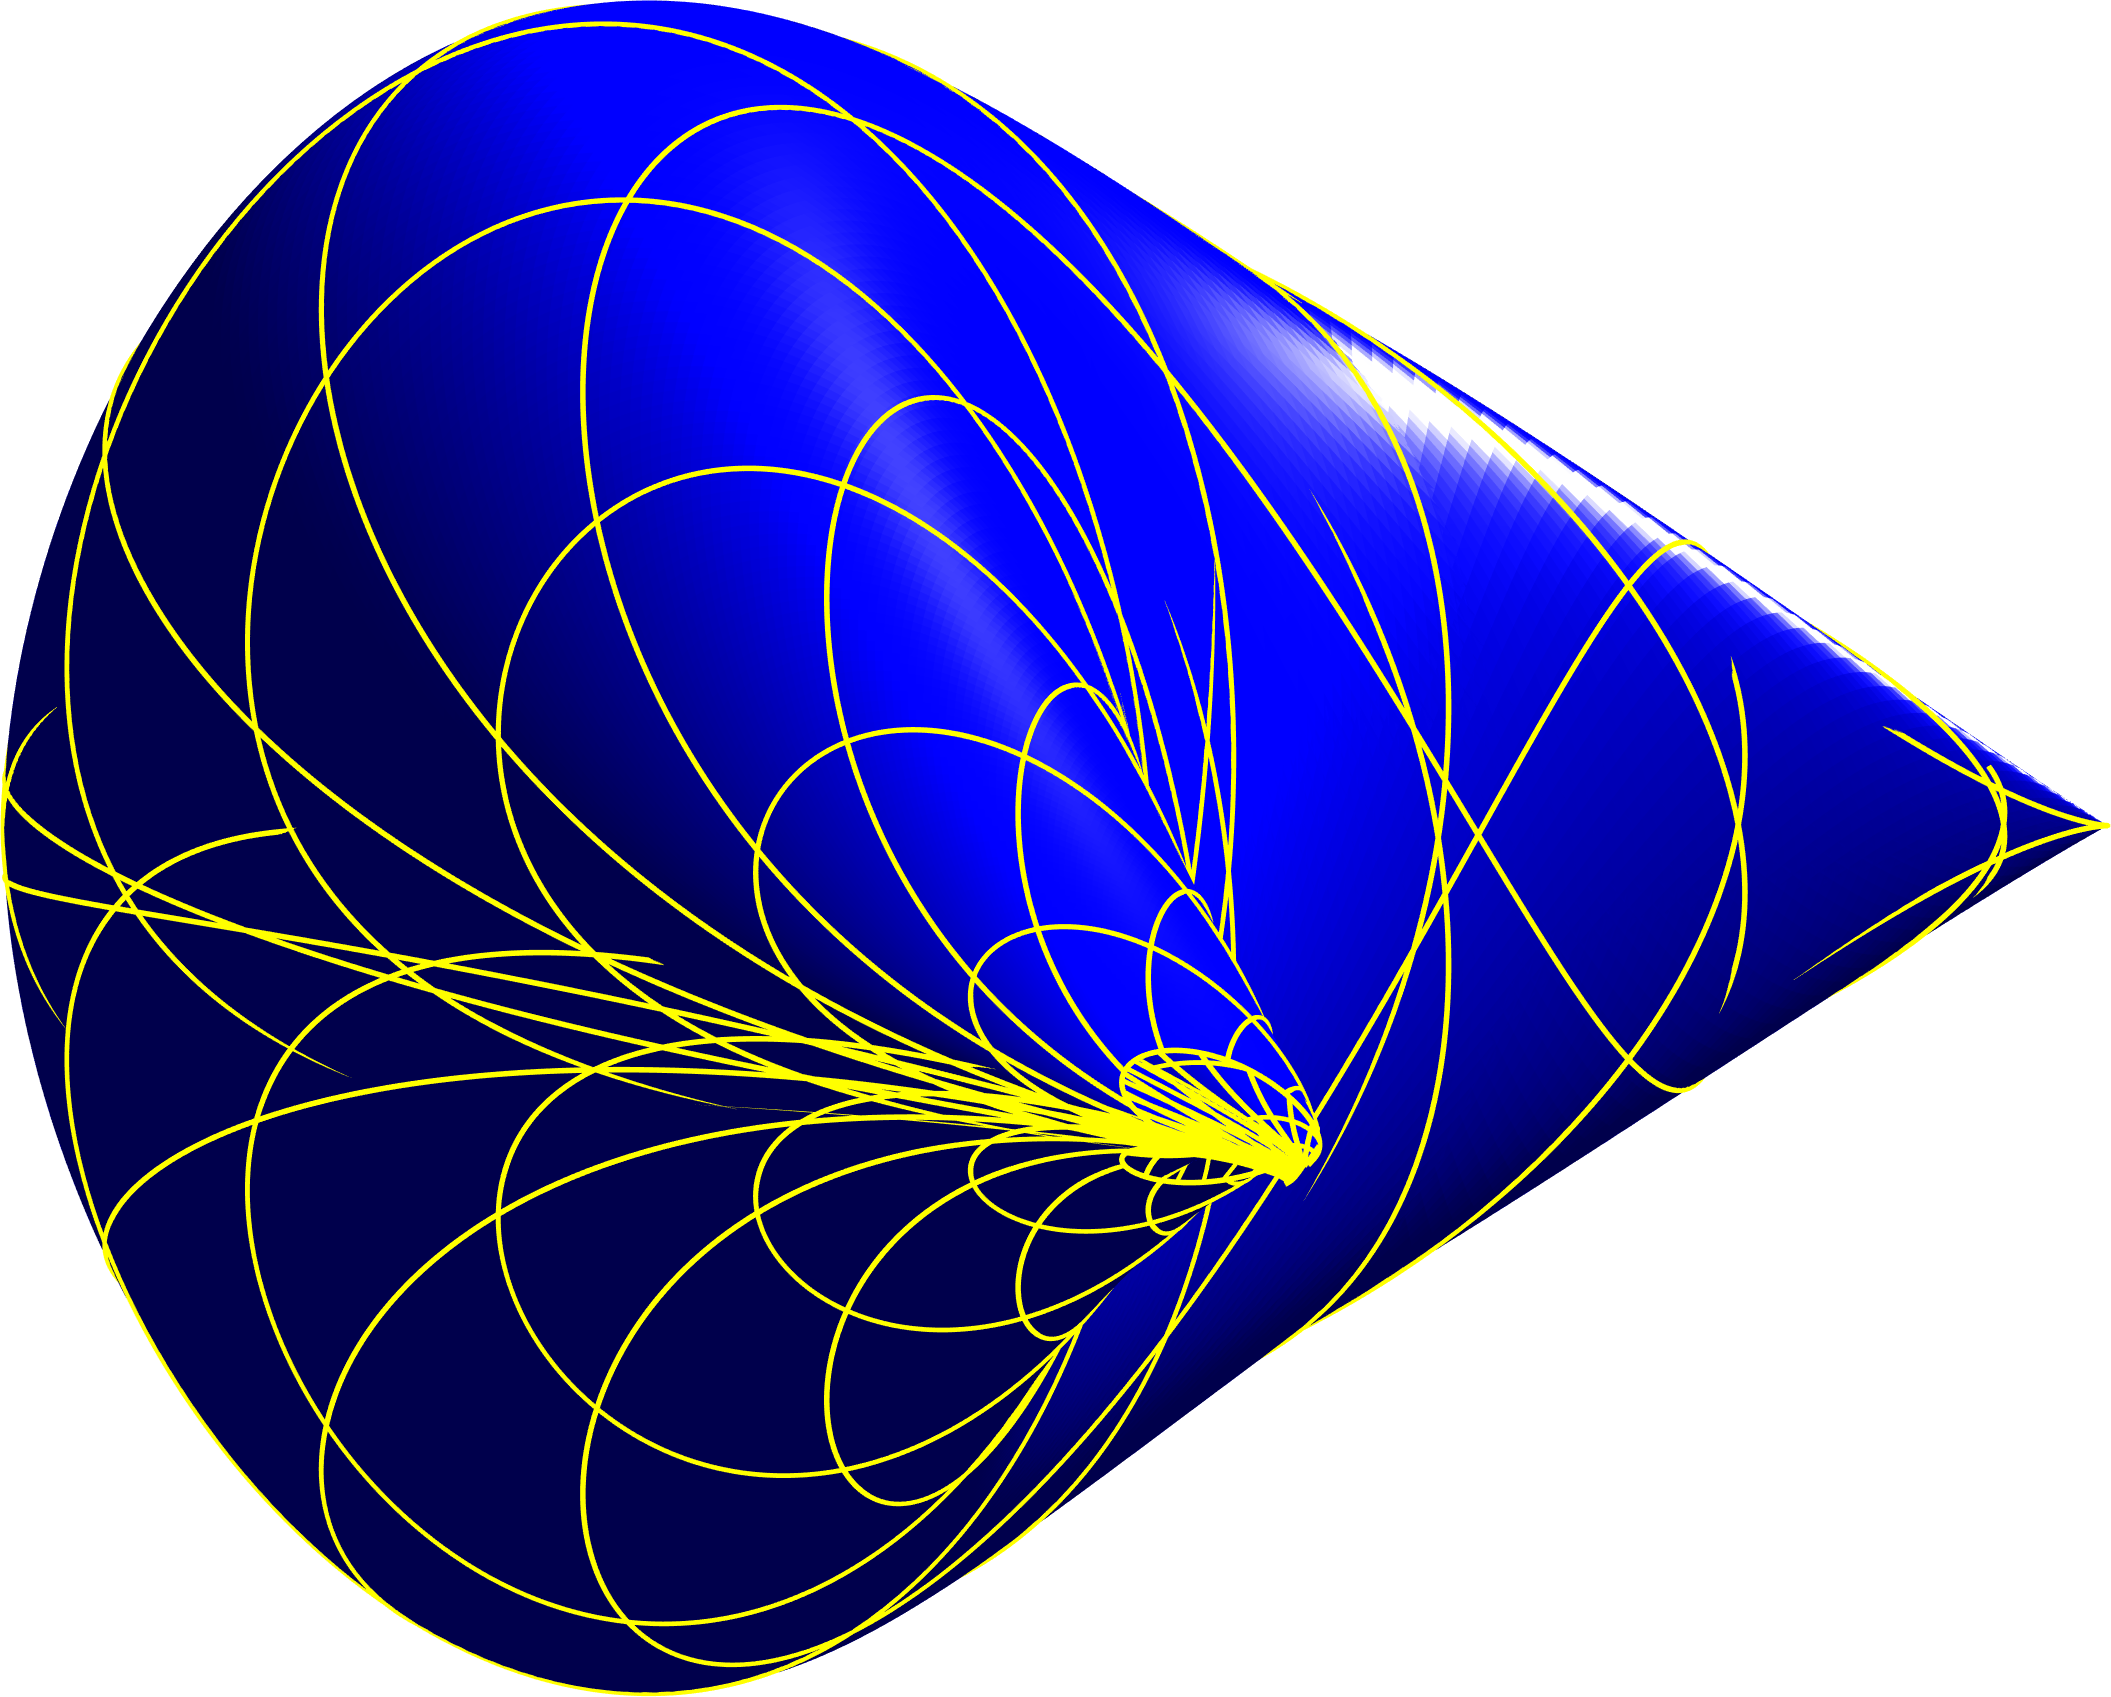
\includegraphics[width=.45\textwidth]{Figs/SE2_signature.png}
\caption{A sample $SE(2)$ Transform and 3D signature.}
\label{fig:SE2}
\end{figure}

\begin{figure}
\centering
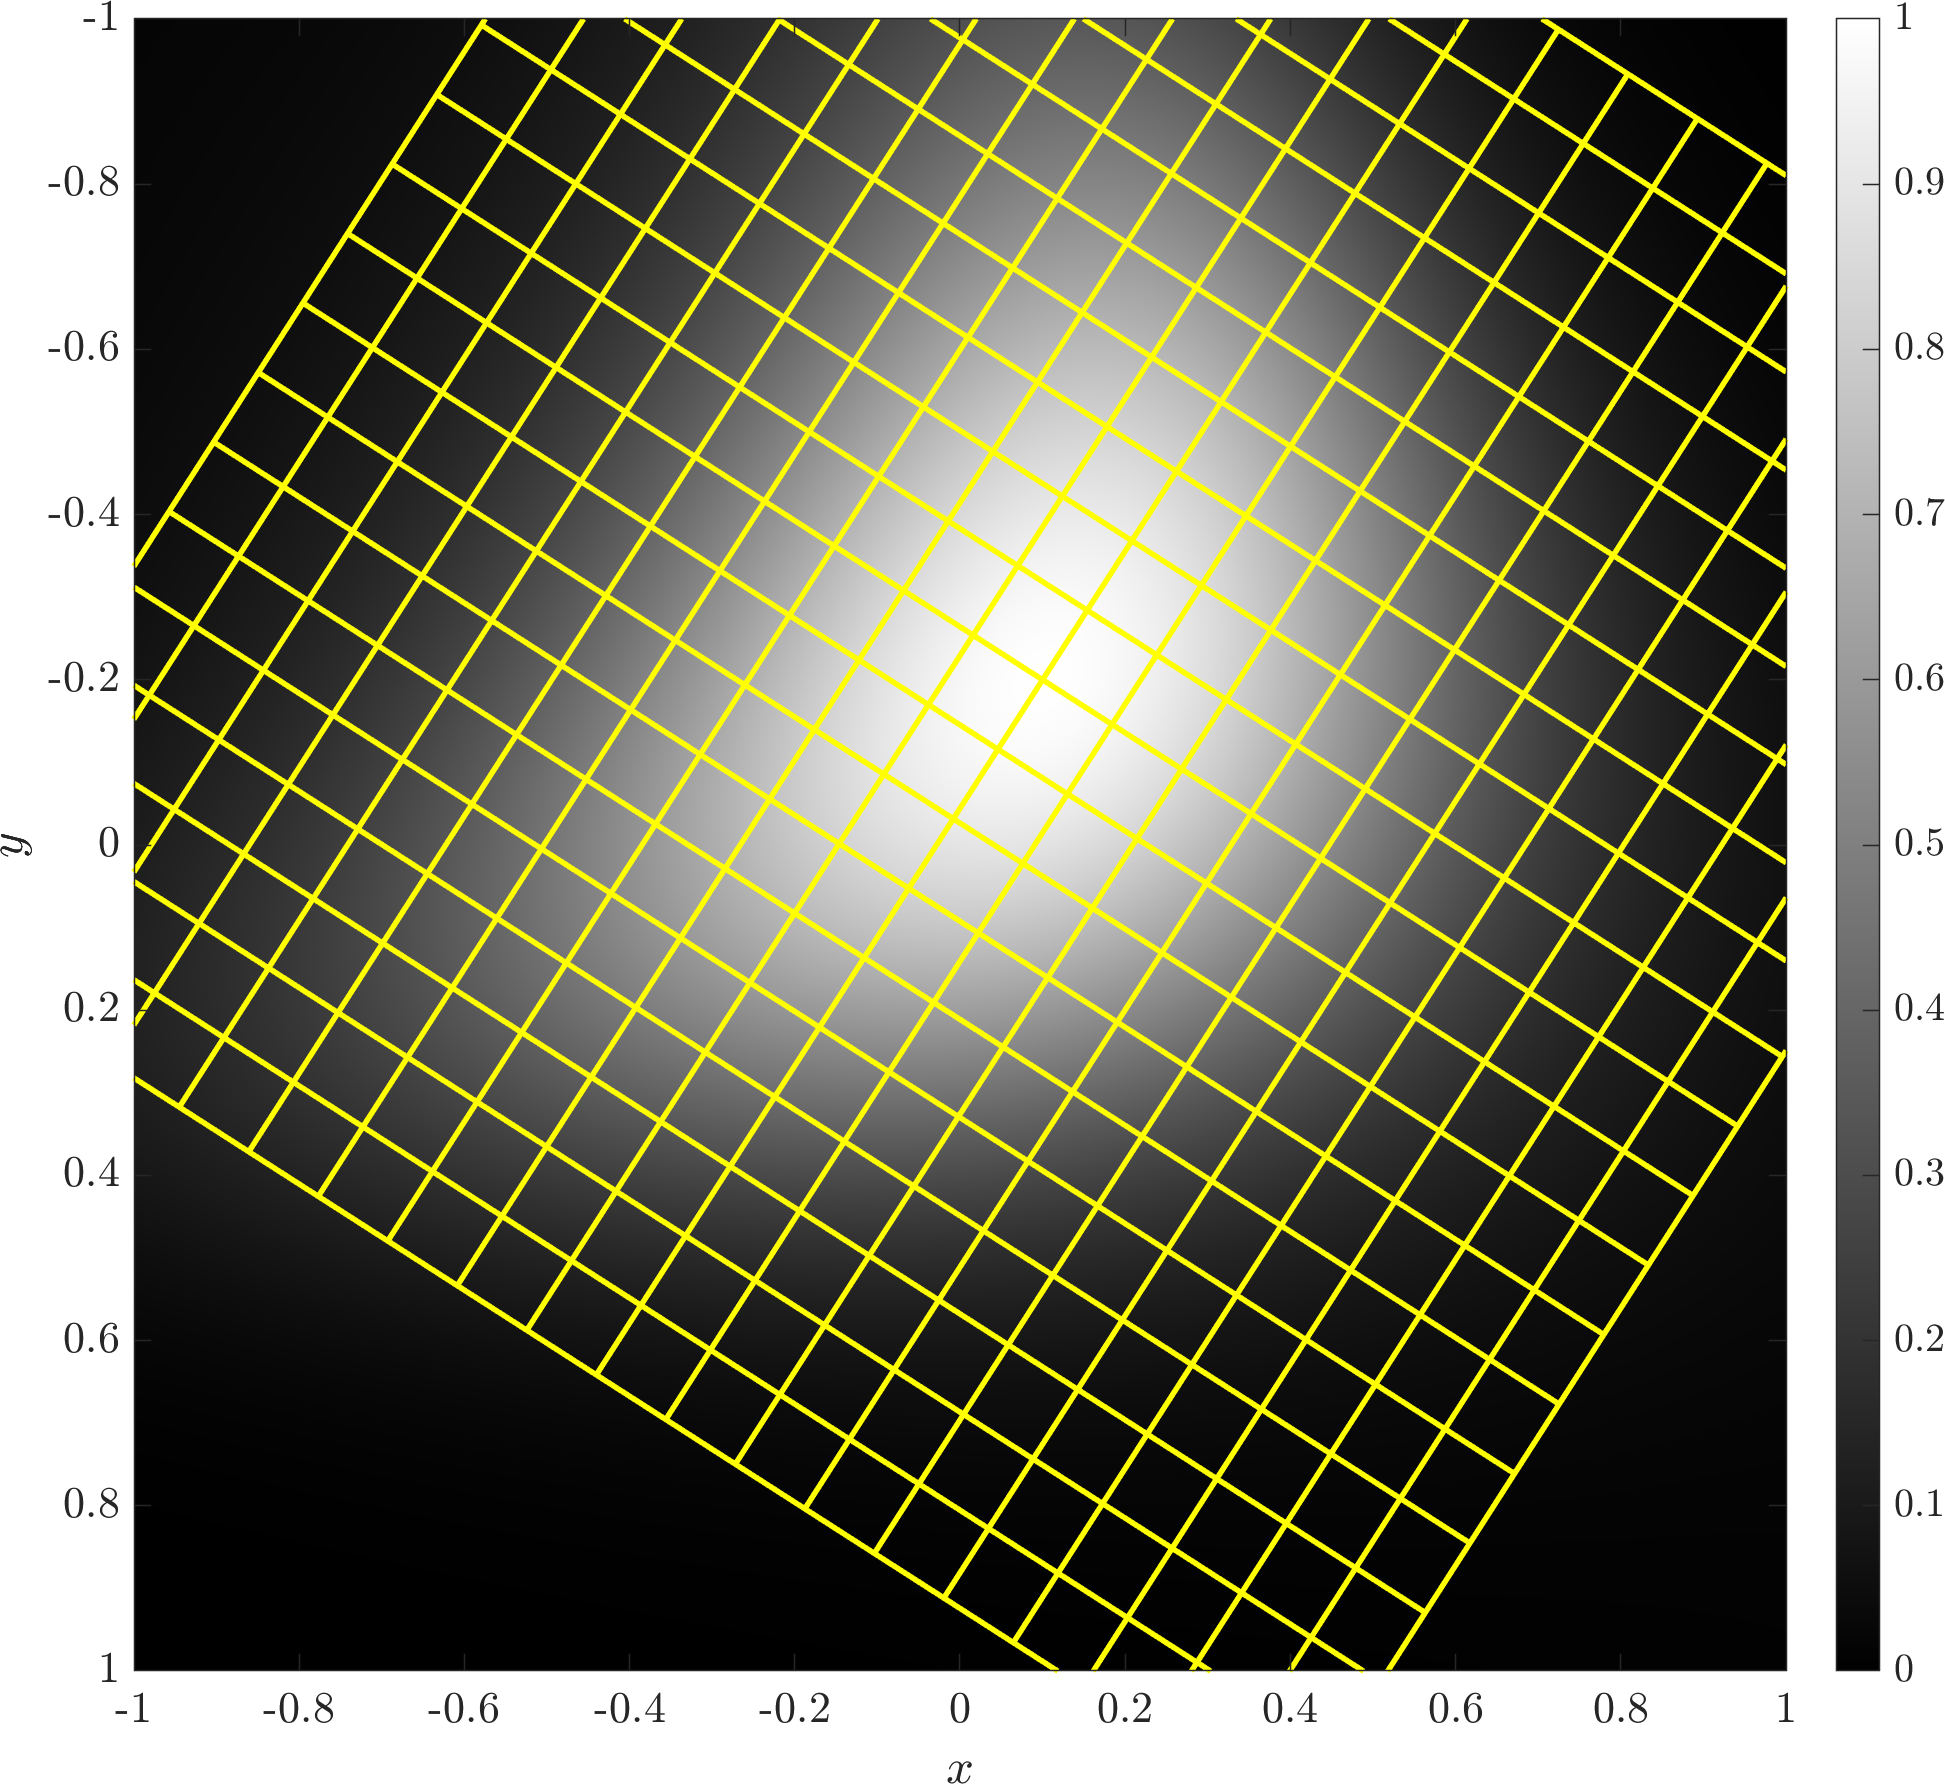
\includegraphics[width=.45\textwidth]{Figs/f_transformed_E2.png}
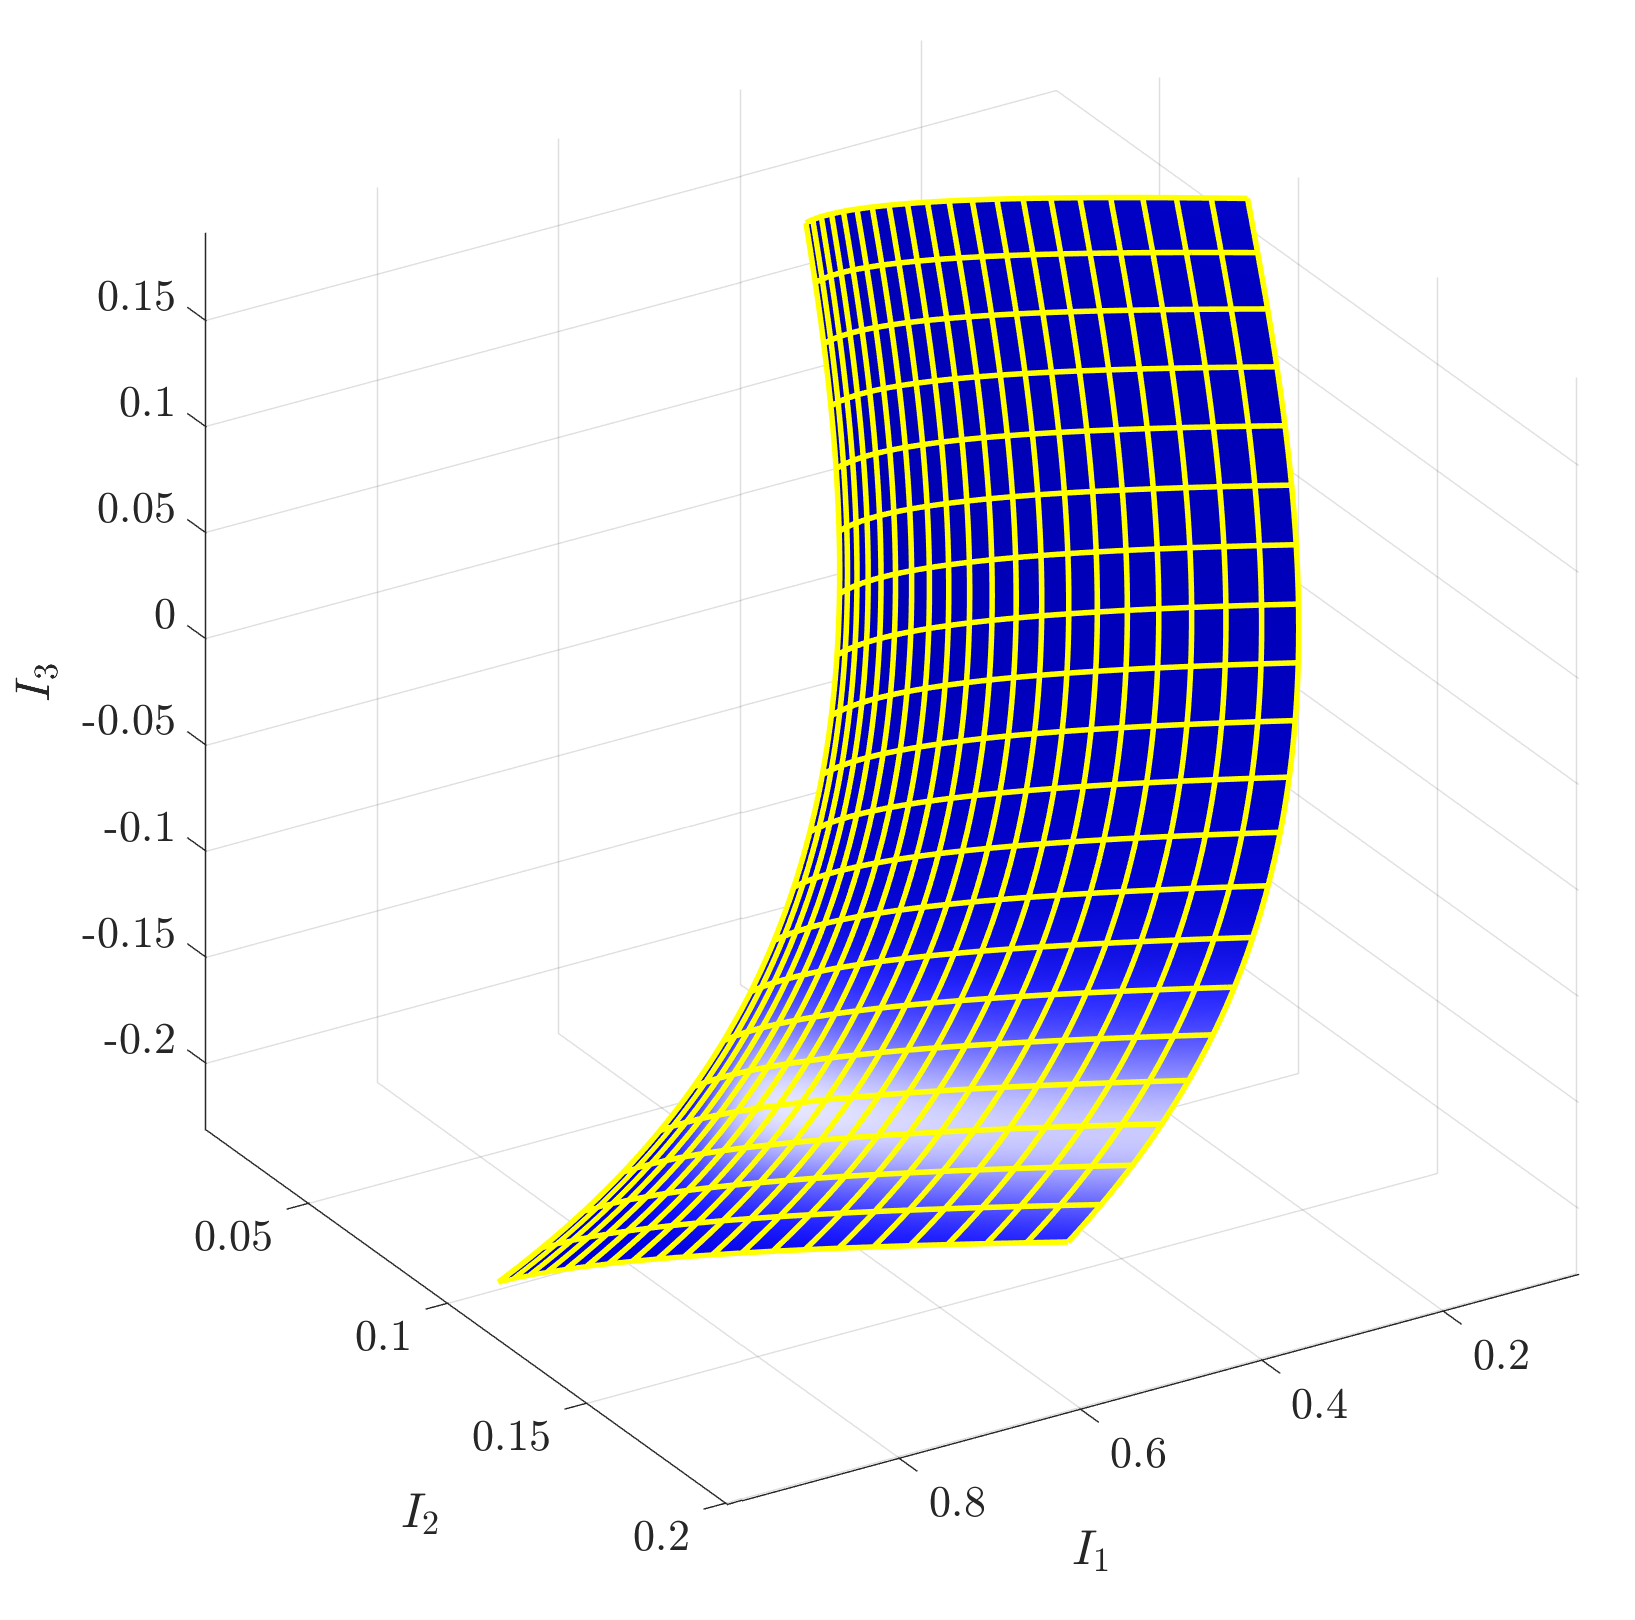
\includegraphics[width=.45\textwidth]{Figs/E2_signature.png}
\caption{A sample $E(2)$ Transform and 3D signature.}
\label{fig:E2}
\end{figure}

\section{Differential invariants through moving frames}\label{sec:movingframes}

So far the methods that we have seen to can construct differential invariants for particular groups are not directly generalisable. It is natural to ask if there is an algorithmic approach that will yield invariants more directly. The answer is a partial yes. There is a general method, based on Cartan's method of moving frames, that is generally applicable, but finding good solutions with it still requires some ingenuity in general. We introduce the method here and then demonstrate its use to find invariants to further groups.

A moving frame is a mapping into a group $\mathcal{G}$ that provides a frame of reference along a curve. Cartan's method of moving frames generalises the concept to a homogeneous space of a Lie group $\mathcal{G}$. When defined on the principal bundle it defines a $\mathcal{G}$-equivariant mapping, which enables one to identify invariants under the action of groups of transformations. The method of moving frames, which originated with Cartan~\cite{Cartan35}  has a long history, as summarised in \cite{Olver2005}. Olver and co-authors, in particular, have popularised the approach and made it applicable to image analysis, see~\cite{Olver2005} for an overview, and the original application paper ~\cite{Calabi1998}. The method is described in detail in~\cite{OlverCIT}.

A (right-) moving frame is a smooth $\mathcal{G}$-equivariant map $\rho : \mathcal{M} \to \mathcal{G}$ such that $\rho (g \cdot z) = \rho(z) \cdot g^{-1}$, where $z \in J^d$. The procedure to construct differential invariants to the action of Lie group $\mathcal{G}$ acting on manifold $\mathcal{M}$ using the method of moving frames is as follows:

\begin{enumerate}
\item Prolong the group action to the jet space of $d$-th order derivatives (using implicit differentiation): $F: J^d \to \mathbb{R}$. 
\item Apply Cartan normalisation:
    \begin{enumerate}
    \item Choose a local cross-section to the group orbits, i.e., a ($d - \dim \mathcal{G}$)-dimensional submanifold $\mathcal{K}$ that intersects transversally at most once with each orbit
    \item $\mathcal{K}$ is specified by $\dim \mathcal{G}$ independent equations $Z_i (z) = c_i$, for $z \in J^d$,  and $Z_i$ scalar-valued functions and $c_i$ constants.
    \item The right moving frame $g = \rho(z)$ is found by solving the normalisation questions $Z_i (g \cdot z) = c_i$ for the group parameters $g$ (in terms of $z$). In other words, the moving frame is the transformation back to the cross-section.
    \end{enumerate}
\item The differential invariants are not affected by the action of the group: $I(g \cdot z) = I(z) \: \forall z \in \mathrm{dom} I$, or equivalently, if it is constant on the orbits. 
\item Hence $F$ is made invariant by transforming it with a group action: $I(z) = F(g \cdot z) |_{g=\rho(z)}$.  
\end{enumerate}

Olver uses the group $SE(2)$ on curves as an example~\cite{Olver}, recovering the Euclidean curvature as a second-order invariant. We continue this example to compute invariants to $SE(2)$ on the plane, before moving on to other planar Lie group examples: $E(2)$, the M\"obius group ($PSL(2,\mathbb{C})$) and the projective group ($PSL(3,\mathbb{R})$). Finally, we apply it to an infinite-dimensional pseudo-Lie group, the conformal diffeomorphisms.

\subsection{The Special Euclidean Group SE(2)}

An element of the special Euclidean group $SE(2)$ acts on an element $(x, y)$ of $\mathbb{R}^2$ to produce $(\bar{x}, \bar{y})$ as:
\begin{equation*}
  \begin{aligned}
    \bar{x} &= x\cos\theta  - y\sin\theta + t_x \\
    \bar{y} &= x\sin\theta  + y\cos\theta + t_y.
  \end{aligned}
\end{equation*}
We prolong the group action to form the jet space $J^2$ with coordinates $(x,
y, f, f_x, f_y, f_{xx}, f_{xy}, f_{yy})$ via the chain rule. The
transformation rule for the derivatives is given by:
\begin{equation}
  \begin{bmatrix}
  \bar f_{\bar x} \\ \bar f_{\bar y} \\ \bar f_{\bar{x}\bar{x}} \\ \bar f_{\bar{x}\bar{y}} \\ \bar f_{\bar{y}\bar{y}}
  \end{bmatrix} = 
  \begin{bmatrix}
 c & -s & 0 & 0 & 0 \\
 s & c & 0 & 0 & 0 \\
0 & 0 & c^2 & -2cs & s^2 \\
0 & 0 & cs & c^2 - s^2 & -cs \\
0 & 0 & s^2 & 2cs & c^2 \\
  \end{bmatrix}
  \begin{bmatrix}
f_x \\ f_y \\ f_{xx} \\ f_{xy} \\ f_{yy} 
  \end{bmatrix},
\label{eqn:SE2}
 \end{equation}
where $c = \cos \theta$ and $s = \sin \theta$. Because the group has three
parameters, we choose the cross section of the group orbits to be $\bar{x}
= 0, \bar{y} = 0, \bar{f}_{\bar{y}} = 0$. We also require that $\bar{f}_{x}
> 0$ to uniquely define the moving frame. Note that the group action is
locally free (away from critical points) when prolonged to $J^1$, however
we prolonged to $J^2$ in order to compute invariants. points. The moving
frame is then given by the prolonged Euclidean transformation that maps an
element of  $J^2$ to this cross section. It can be thought of as rotating
the image about that point so that its gradient is pointing in the positive
$x$ direction, and then translating the image so the point is mapped to the
origin. 

This choice of moving frame gives $\cos\theta = f_x/\lVert\nabla f\rVert$
and $\sin\theta = -f_y/\lVert \nabla f \rVert$. The parameters $t_x, t_y$
are then $t_x = -x\cos\theta + y\sin\theta$ and $t_y = -x\sin\theta -
y\cos\theta$, however these have no effect on the derivatives, and will
henceforth be ignored.

The remaining elements not fixed by the cross section, $\bar{f}$,
$\bar{f}_{\bar{x}}$, $\bar{f}_{\bar{x}\bar{x}}$,
$\bar{f}_{\bar{x}\bar{y}}$, and $\bar{f}_{\bar{y}\bar{y}}$ are therefore
all invariant. This gives the following set of invariants:
\begin{equation}\label{eq:se2invariants}
\begin{aligned}
  I_0 &= f \\
  I_1 &= f_x^2 + f_y^2 & &(= \bar{f}_{\bar{x}}^2)\\
  I_2 &= f_x^2 f_{xx} + 2 f_x f_y f_{xy} + f_y^2 f_{yy} &&(= I_1\bar{f}_{\bar{x}\bar{x}}) \\
  I_3 &= f_x f_y (f_{yy} - f_{xx}) + f_{xy} (f_x^2 - f_y^2) &&(= I_1\bar{f}_{\bar{x}\bar{y}})\\
  I_4 &= f_y^2 f_{xx} - 2 f_x f_y f_{xy} + f_x^2 f_{yy} &&(= I_1\bar{f}_{\bar{y}\bar{y}}).
\end{aligned}
\end{equation}
Note that we multiplied each of the second derivative invariants by $I_1$
so that they would decay smoothly to zero at critical points.

\todo[inline]{c.f. transvectant formulae}

\subsection{The Euclidean Group E(2)}
An element of the Euclidean group $E(2)$ maps an element $(x, y)$ of
$\mathbb{R}^2$ to $(\bar{x}, \bar{y})$ as 
\begin{equation*}
  \begin{aligned}
    \bar{x} &=  x\varepsilon\cos\theta  - y\varepsilon\sin\theta + t_x \\
    \bar{y} &= x\sin\theta  + y\cos\theta + t_y.
  \end{aligned}
\end{equation*}
where $\varepsilon \in \{-1, 1\}$ and the remaining parameters are the same
as for $SE(2)$. If $\varepsilon = 1$ it is a rigid transformation, and if
$\varepsilon = -1$ it contains a reflection.

This time, the group action is not free on $J^1$ (with elements of the form
$(x, y, f, f_x, f_y)$) away from critical points because there are two
possible transformations that map to the cross section $(0, 0, \bar{f},
\bar{f}_{\bar{x}}, 0)$ where $\bar{f}_{\bar{x}} > 0$, one that reflects the
gradient into the positive $x$ direction, and one that rotates. 

We again prolong the group action to $J^2$, but this time we expect to need
to use a second derivative term to determine $\varepsilon$ for the moving
frame. The derivative transformations are given by:
\begin{equation}
  \begin{bmatrix}
  \bar f_{\bar x} \\ \bar f_{\bar y} \\ \bar f_{\bar{x}\bar{x}} \\ \bar f_{\bar{x}\bar{y}} \\ \bar f_{\bar{y}\bar{y}}
  \end{bmatrix} = 
  \begin{bmatrix}
 \varepsilon c & -\varepsilon s & 0 & 0 & 0 \\
 s & c & 0 & 0 & 0 \\
0 & 0 & c^2 & -2cs & s^2 \\
0 & 0 & \varepsilon cs & \varepsilon(c^2 - s^2) & -\varepsilon cs \\
0 & 0 & s^2 & 2cs & c^2 \\
  \end{bmatrix}
  \begin{bmatrix}
f_x \\ f_y \\ f_{xx} \\ f_{xy} \\ f_{yy} 
  \end{bmatrix},
\label{eqn:E2prolongation}
\end{equation}
where again $c = \cos\theta$ and $s = \sin\theta$.  

We begin by choosing the same cross section as for $SE(2)$, namely $\bar{x} = 0,
\bar{y} = 0, \bar{f}_{\bar{y}} = 0, \bar{f}_{\bar{x}} > 0$. This gives
$\cos\theta = \varepsilon f_x / \lVert \nabla f \rVert$ and $\sin\theta =
-\varepsilon f_y / \lVert \nabla f \rVert$. Under this transformation,
regardless of whether $\varepsilon = 1$ or $\varepsilon = -1$, the
derivative $\bar{f}_{\bar{x}} = \lVert \nabla f \rVert$. We need a second
derivative term to resolve the choice of $\varepsilon$ for the moving
frame. The only second derivative term in which $\varepsilon$ appears is
the $\bar{f}_{\bar{x}\bar{y}}$ term. Substituting in for $\cos\theta,
\sin\theta$, we see that:
\begin{equation*}
    \bar{f}_{\bar{x}\bar{y}} = \frac{\varepsilon(f_xf_y(f_{yy} - f_{xx}) + (f_x^2 -
    f_y^2)f_{xy})}{f_x^2 + f_y^2}.
\end{equation*}
This suggests choosing $\varepsilon$ to make $\bar{f}_{\bar{x}\bar{y}} \ge
0$. We can then list the invariants:
\begin{equation}\label{eq:e2invariants}
\begin{aligned}
  I_0 &= f \\
  I_1 &= f_x^2 + f_y^2 & &(= \bar{f}_{\bar{x}}^2)\\
  I_2 &= f_x^2 f_{xx} + 2 f_x f_y f_{xy} + f_y^2 f_{yy} &&(= I_1\bar{f}_{\bar{x}\bar{x}}) \\
  I_3 &= \lvert f_x f_y (f_{yy} - f_{xx}) + f_{xy} (f_x^2 - f_y^2)\rvert
  &&(= I_1\lvert \bar{f}_{\bar{x}\bar{y}}\rvert)\\
  I_4 &= f_y^2 f_{xx} - 2 f_x f_y f_{xy} + f_x^2 f_{yy} &&(= I_1\bar{f}_{\bar{y}\bar{y}}).
\end{aligned}
\end{equation}
Notice that most, but not all of the $SE(2)$ invariants
\eqref{eq:se2invariants} are also $E(2)$ invariants. We again multiply
through the invariants by $I_1$ so that they decay smoothly at critical
points.

These invariants are a functionally independent, complete, set of polynomial differential invariants up to second derivatives. Note that the invariants found previously by tensor contraction (\ref{eq:se2}) can be expressed in terms of these:
\begin{align*}
  f = f &= I_0 \\
  f_if_i = f_x^2 + f_y^2 &= I_1 \\
  f_{ii} = f_{xx}^2 + f_{yy}^2 &= \frac{I_2 + I_4}{I_1} \\
  f_{ij} f_{ij} = f_{xx}^2 + 2f_{xy}^2 + f_{yy}^2 &= I_2\\
  f_i f_j f_{ij} = f_x^2 f_{xx} + 2f_x f_y f_{xy} + f_y^2 f_{yy} &= \frac{I_2^2 + I_4^2 + 2I_3^2}{I_1^2}.
\end{align*}

\subsection{The M\"{o}bius Group}

The M\"obius group $\mathrm{PSL}(2,\mathbb{C})$ acts on the Riemann sphere
$\overline{\mathbb{C}} = \mathbb{C}\cup\infty$ by:
\begin{equation} 
\phi\colon \overline{\mathbb{C}} \to \overline{\mathbb{C}},\quad \phi(z) = \frac{\alpha z + \beta}{\gamma z + \delta},\quad \alpha,\beta,\gamma,\delta\in\mathbb{C}, \quad
\alpha\delta-\beta\gamma\ne 0.
\end{equation}

Identifying $\R^2$ with $\mathbb{C}$, the M\"obius group is a real 6-dimensional local Lie group acting on $\mathbb{R}^2$.
It is the smallest nonlinear planar group that contains $SE(2)$, and it also has direct applications in image processing since it arises in the {\em conformal camera} model of vision, in which scenes are projected radially onto a sphere \cite{Lenz1990,Turski2004}; it is also the set of biholomorphic maps of the Riemann sphere. 
%Different shapes may be related by M\"obius transformations, as is explored by Petukhov \cite{petukhov1989non} for biological objects: in one example, the human skull grows approximately by M\"obius transformations.  Note also that Thompson \cite{thompson1942growth} famously deformed images of one species to match those of another, many of his examples using conformal mappings, and thus may be approximated (or even determined by) M\"obius transformations. Discussing this work, Milnor \cite{milnor2010growth}  argued that ``The geometrically simplest way to change the relative size of different body parts would be by a conformal transformation. It seems plausible that this simplest solution will often be the most efficient, so that natural selection tend to choose it.'' (Milnor was thinking of 3D conformal transformations, whose restriction to 2D is the M\"obius transformations.)

We are free to take $\delta=1$. Then $\bar f = f$ means that $z$ is translated to $\beta$; we can therefore take $\beta=0$. This leaves 4 group parameters $a,b,c,d$, where $\alpha = a + i b$, $\gamma = c + i d$, to be determined as follows. We prolong the action to second derivatives of $f$, which is sufficient to allow the group to act freely. There are 5 derivatives of $f$ up to order 2, so there will be at least 1 invariant. In order to find further invariants the prolongation to 3rd derivatives is required, which will result in at least another four invariants. %There are 9 derivatives of $f$ of order 1, 2, and 3, so there must be at least 5 invariants.
\todo[inline]{General thm for this earlier...}

The prolonged action is:
\begin{equation}
\arraycolsep=1.4pt
\left[
\begin{array}{c}
  \bar f_{\bar x} \\ \bar f_{\bar y} \\ \bar f_{\bar x \bar x} \\ \bar f_{\bar x \bar y} \\ \bar f_{\bar y \bar y} 
 \end{array}
 \right]
 = 
\left[
\begin{array}{ccccc}
 a & b & 0 & 0 & 0 \\
 -b & a & 0 & 0 & 0 \\
 2\mu & -2 \rho & a^2 & 2 a b & b^2 \\
 2 \rho & 2\mu & -a b & a^2\!-b^2 & a b \\
 -2\mu & 2 \rho & b^2 & -2 a b & a^2 \\
\end{array}
\right]\left[
\begin{array}{c}
f_x \\ f_y \\ f_{xx} \\ f_{xy} \\ f_{yy} \\
 \end{array}
 \right].
\label{eqn:mobius}
 \end{equation}

\noindent where $\mu = b d - a c$ and $\rho = b c + a d$.

%\begin{equation}
%\arraycolsep=1.4pt
%\left(
%\begin{array}{c}
  %\bar f_x \\ \bar f_y \\ \bar f_{xx} \\ \bar f_{xy} \\ \bar f_{yy} \\ \bar f_{xxx} \\ \bar f_{xxy} \\ \bar f_{xyy} \\ \bar f_{yyy} 
 %\end{array}
 %\right)
 %= 
%\left(
%\begin{array}{ccccccccc}
 %a & b & 0 & 0 & 0 & 0 & 0 & 0 & 0 \\
 %-b & a & 0 & 0 & 0 & 0 & 0 & 0 & 0 \\
 %2\mu & -2 \rho & a^2 & 2 a b & b^2 & 0 & 0 & 0 & 0 \\
 %2 \rho & 2\mu & -a b & a^2\!-b^2 & a b & 0 & 0 & 0 & 0 \\
 %-2\mu & 2 \rho & b^2 & -2 a b & a^2 & 0 & 0 & 0 & 0 \\
 %-6 (2 b c d+a \lambda) & 6 (2 a c d-b\lambda) & 6 a \mu &
  %M_{64}  & -6 b \rho & a^3 & 3 a^2 b & 3 a b^2 & b^3 \\
 %-6 (2 a c d-b\lambda) & -6 (2 b c d+a \lambda) & M_{73}& M_{74} & 
 %M_{75} & -a^2 b & a^3\!-2 a b^2 & 2
   %a^2 b\!-b^3 & a b^2 \\
 %6 (2 b c d+a \lambda) & -6 (2 a c d-b\lambda) & M_{83} & M_{84} & M_{85} & a b^2 & b^3\!-2
   %a^2 b & a^3\!-2 a b^2 & a^2 b \\
 %6 (2 a c d-b\lambda) & 6 (2 b c d+a \lambda) & 6 b \mu & 
  %M_{94} & 6 a \rho & -b^3 & 3 a b^2 & -3 a^2 b & a^3 \\
%\end{array}
%\right)\left(
%\begin{array}{c}
%f_x \\ f_y \\ f_{xx} \\ f_{xy} \\ f_{yy} \\ f_{xxx} \\ f_{xxy} \\ f_{xyy} \\ f_{yyy} 
 %\end{array}
 %\right).
%\label{eqn:mobius}
 %\end{equation}
 %where
 %\begin{equation*}
 %\begin{array}{lll}
%M_{64}=-12abc+6d(a^2-b^2), & 
%M_{73}=4 d a^2+6 b c a-2 b^2 d, & 
%M_{74}=-6 c a^2+12 b d a+6 b^2 c, \\
 %M_{75}=-2 d a^2-6 b c a+4 b^2 d, &
 %M_{83}=2 c a^2-6 b d a-4 b^2 c, &
 %M_{84}=6 (d a^2+2 b c a-b^2 d),\\
 %M_{85}=-4 c a^2+6 b d a+2 b^2 c,& 
 %M_{94}= -12a b d + 6c(a^2-b^2),\\
%\lambda=d^2-c^2, & 
%\mu = b d - a c, & 
%\rho = b c + a d.
%\end{array}
%\end{equation*}

The moving frame calculation is then:
\begin{enumerate}
\item The frame $\bar f_{\bar x}=1$, $\bar f_{\bar y}=0$ determines the group parameters:
$$ a = f_x/(f_x^2 + f_y^2),\quad b = f_y/(f_x^2 f_y^2).$$

\item The frame $\bar f_{\bar x \bar y}=\bar f_{\bar y \bar y}=0$ determines the next group parameters:
$$ c = (2 f_xf_yf_{xyy} - f_{xx}f_y^2 - f_{yy}f_x^2)/(2 f_x^2 + f_y^2)^2$$
$$ d = (f_{xy}f_x^2 - f_x f_y f_{xx} - f_{xy}f_y^2 - f_{yy} f_x f_y)/(2 f_x^2 + f_y^2)^2.$$

\item The second-order invariant is then given by $\bar f_{\bar x \bar x}$ using Equation~(\ref{eqn:mobius}); it is:
$$\bar f_{\bar x \bar x} = \frac{f_{xx}+f_{yy}}{f_x^2 + f_y^2}.$$
\end{enumerate}

%It is clear that there must be 2 syzygies between the relative invariants $J_1,\dots,J_4,K_1,\dots,K_4$.
%They are easily found algebraically to be
%$$K_2 = -K_4 + J_1 J_4$$
%and
%$$K_3=-K_1 +J_1 J_3 + 2 J_1^2 J_2^2.$$

The four third-order invariants can be deduced from the moving frame. They are rational functions with numerators of degree 6 and denominators $(f_x^2 + f_y^2)^4$, and are relative invariants of weight 8.  Clearing denominators so as to work with polynomials, we choose $M_1 = (f_{xx} + f_{yy})^4$ and two of the four third-order invariants to form a M\"obius signature $(M_1, M_2, M_3)$, where: 
$$M_2=
f_y ^5 f_{yyy} + \frac{9}{2} f_y ^2 f_{yy}^2 f_x ^2 + 
 f_y ^3 f_{yyy} f_x ^2 + \frac{3}{2} f_{yy}^2 f_x ^4 - 
 9 f_y ^3 f_{yy} f_x  f_{xy} + 
 3 f_y  f_{yy} f_x ^3 f_{xy} + \frac{3}{2} f_y ^4 f_{xy}^2 - 
 9 f_y ^2 f_x ^2 f_{xy}^2 + \frac{3}{2} f_z ^4 f_{xy}^2 + 
 3 f_y ^4 f_x  f_{xyy} + 3 f_y ^2 f_x ^3 f_{xyy} + 
 3 f_y ^4 f_{yy} f_{xx} + 3 f_{yy} f_x ^4 f_{xx} + 
 3 f_y ^3 f_x  f_{xy} f_{xx} - 
 9 f_y  f_x ^3 f_{xy} f_{xx} + \frac{3}{2} f_y ^4 f_{xx}^2 + 
 \frac{9}{2} f_y ^2 f_x ^2 f_{xx}^2 + 3 f_y ^3 f_x ^2 f_{xxy} + 
 3 f_y  f_x ^4 f_{xxy} + f_y ^2 f_x ^3 f_{xxx} + 
 f_x ^5 f_{xxx}, 
 $$
 
 $$M_3=-3 f_y  f_{yy}^2 f_x ^3 + 
 f_y ^2 f_{yyy} f_x ^3 + f_{yyy} f_x ^5 + 
 9 f_y ^2 f_{yy} f_x ^2 f_{xy} - 
 3 f_{yy} f_x ^4 f_{xy} - 6 f_y ^3 f_x  f_{xy}^2 + 
 6 f_y  f_x ^3 f_{xy}^2 - 3 f_y ^3 f_x ^2 f_{xyy} - 
 3 f_y  f_x ^4 f_{xyy} - 3 f_y ^3 f_{yy} f_x  f_{xx} + 
 3 f_y  f_{yy} f_x ^3 f_{xx} + 3 f_y ^4 f_{xy} f_{xx} - 
 9 f_y ^2 f_x ^2 f_{xy} f_{xx} + 
 3 f_y ^3 f_x  f_{xx}^2 + 3 f_y ^4 f_x  f_{xxy} + 
 3 f_y ^2 f_x ^3 f_{xxy} - f_y ^5 f_{xxx} - 
 f_y ^3 f_x ^2 f_{xxx}.
$$

The image $f$ and these 3 relative invariants of weight 8 provide a three-dimensional signature; an example is shown in Figure~\ref{fig:mobius}, although note that it is singular when $f_x=f_y=f_{xx}+f_{yy}=0$, a codimension 1 phenomenon for images. 

%In previous work \cite{mobius}, two independent 3rd order M\"obius invariants were calculated
%from the classical M\"obius geometry of curves. Namely, the M\"obius arclength 
%of a curve is $\sqrt{|\kappa_s|}ds$, were $ds$ is Euclidean arclength. Under any conformal map $\phi$,
%both $ds$ and $1/\|\nabla f\|$ scale by $|\phi'|$. The sign of $\kappa_s$ is also  invariant,
%hence $\kappa_s/\|\nabla f\|^2$ is  invariant for any invariant curve. 
%Calculating this invariant
%for the level sets of $f$ and for their orthogonal curves yields two invariants of $f$ that
%we call $\lambda_t$ and $\lambda_n$, respectively. Writing 
%them out in full and comparing to the invariants founds above shows that they are related very simply, by

%$$ \frac{K_2}{\|\nabla f\|^8} = \lambda_t$$
%$$\frac{K_4}{\|\nabla f\|^8} =\lambda_n$$

%We do not know of any equivalent characterization of the invariants $K_1$, $K_3$ in
%terms of classical M\"obius geometry.

%We now have that
%$$ (J_1^4, J_2^4, J_1 J_3, J_1 J_4, K_1, K_4)$$
%are 6 relative invariants of weight 8. Projecting any subset to a sphere provides a M\"obius signature.
%For example, the image $f$ together with the projection of $(J_1^4, J_2^4, K_1)$ provides a 3-dimensional signature.
%Any such signature that includes $J_1$ and $J_2$ is 

\begin{figure}
\centering
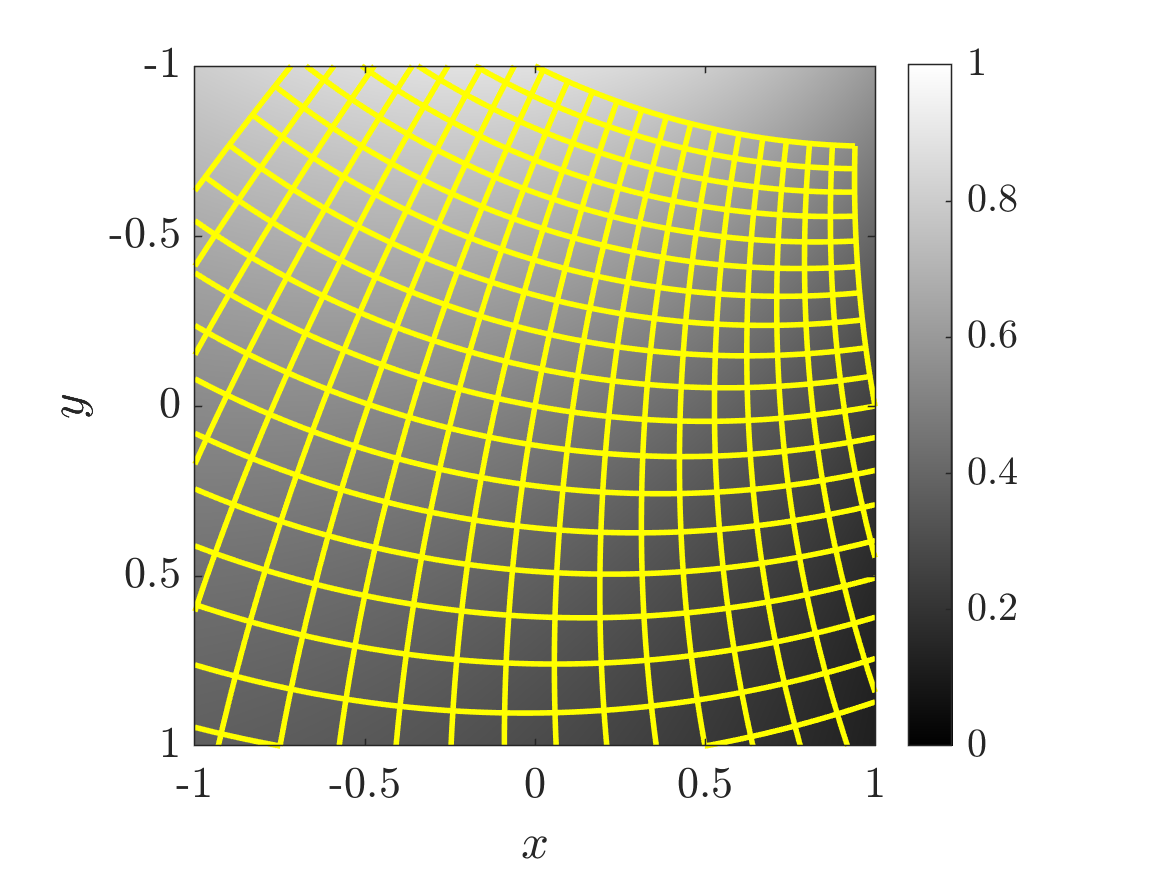
\includegraphics[width=.45\textwidth]{Figs/f_transformed_Mobius.png}
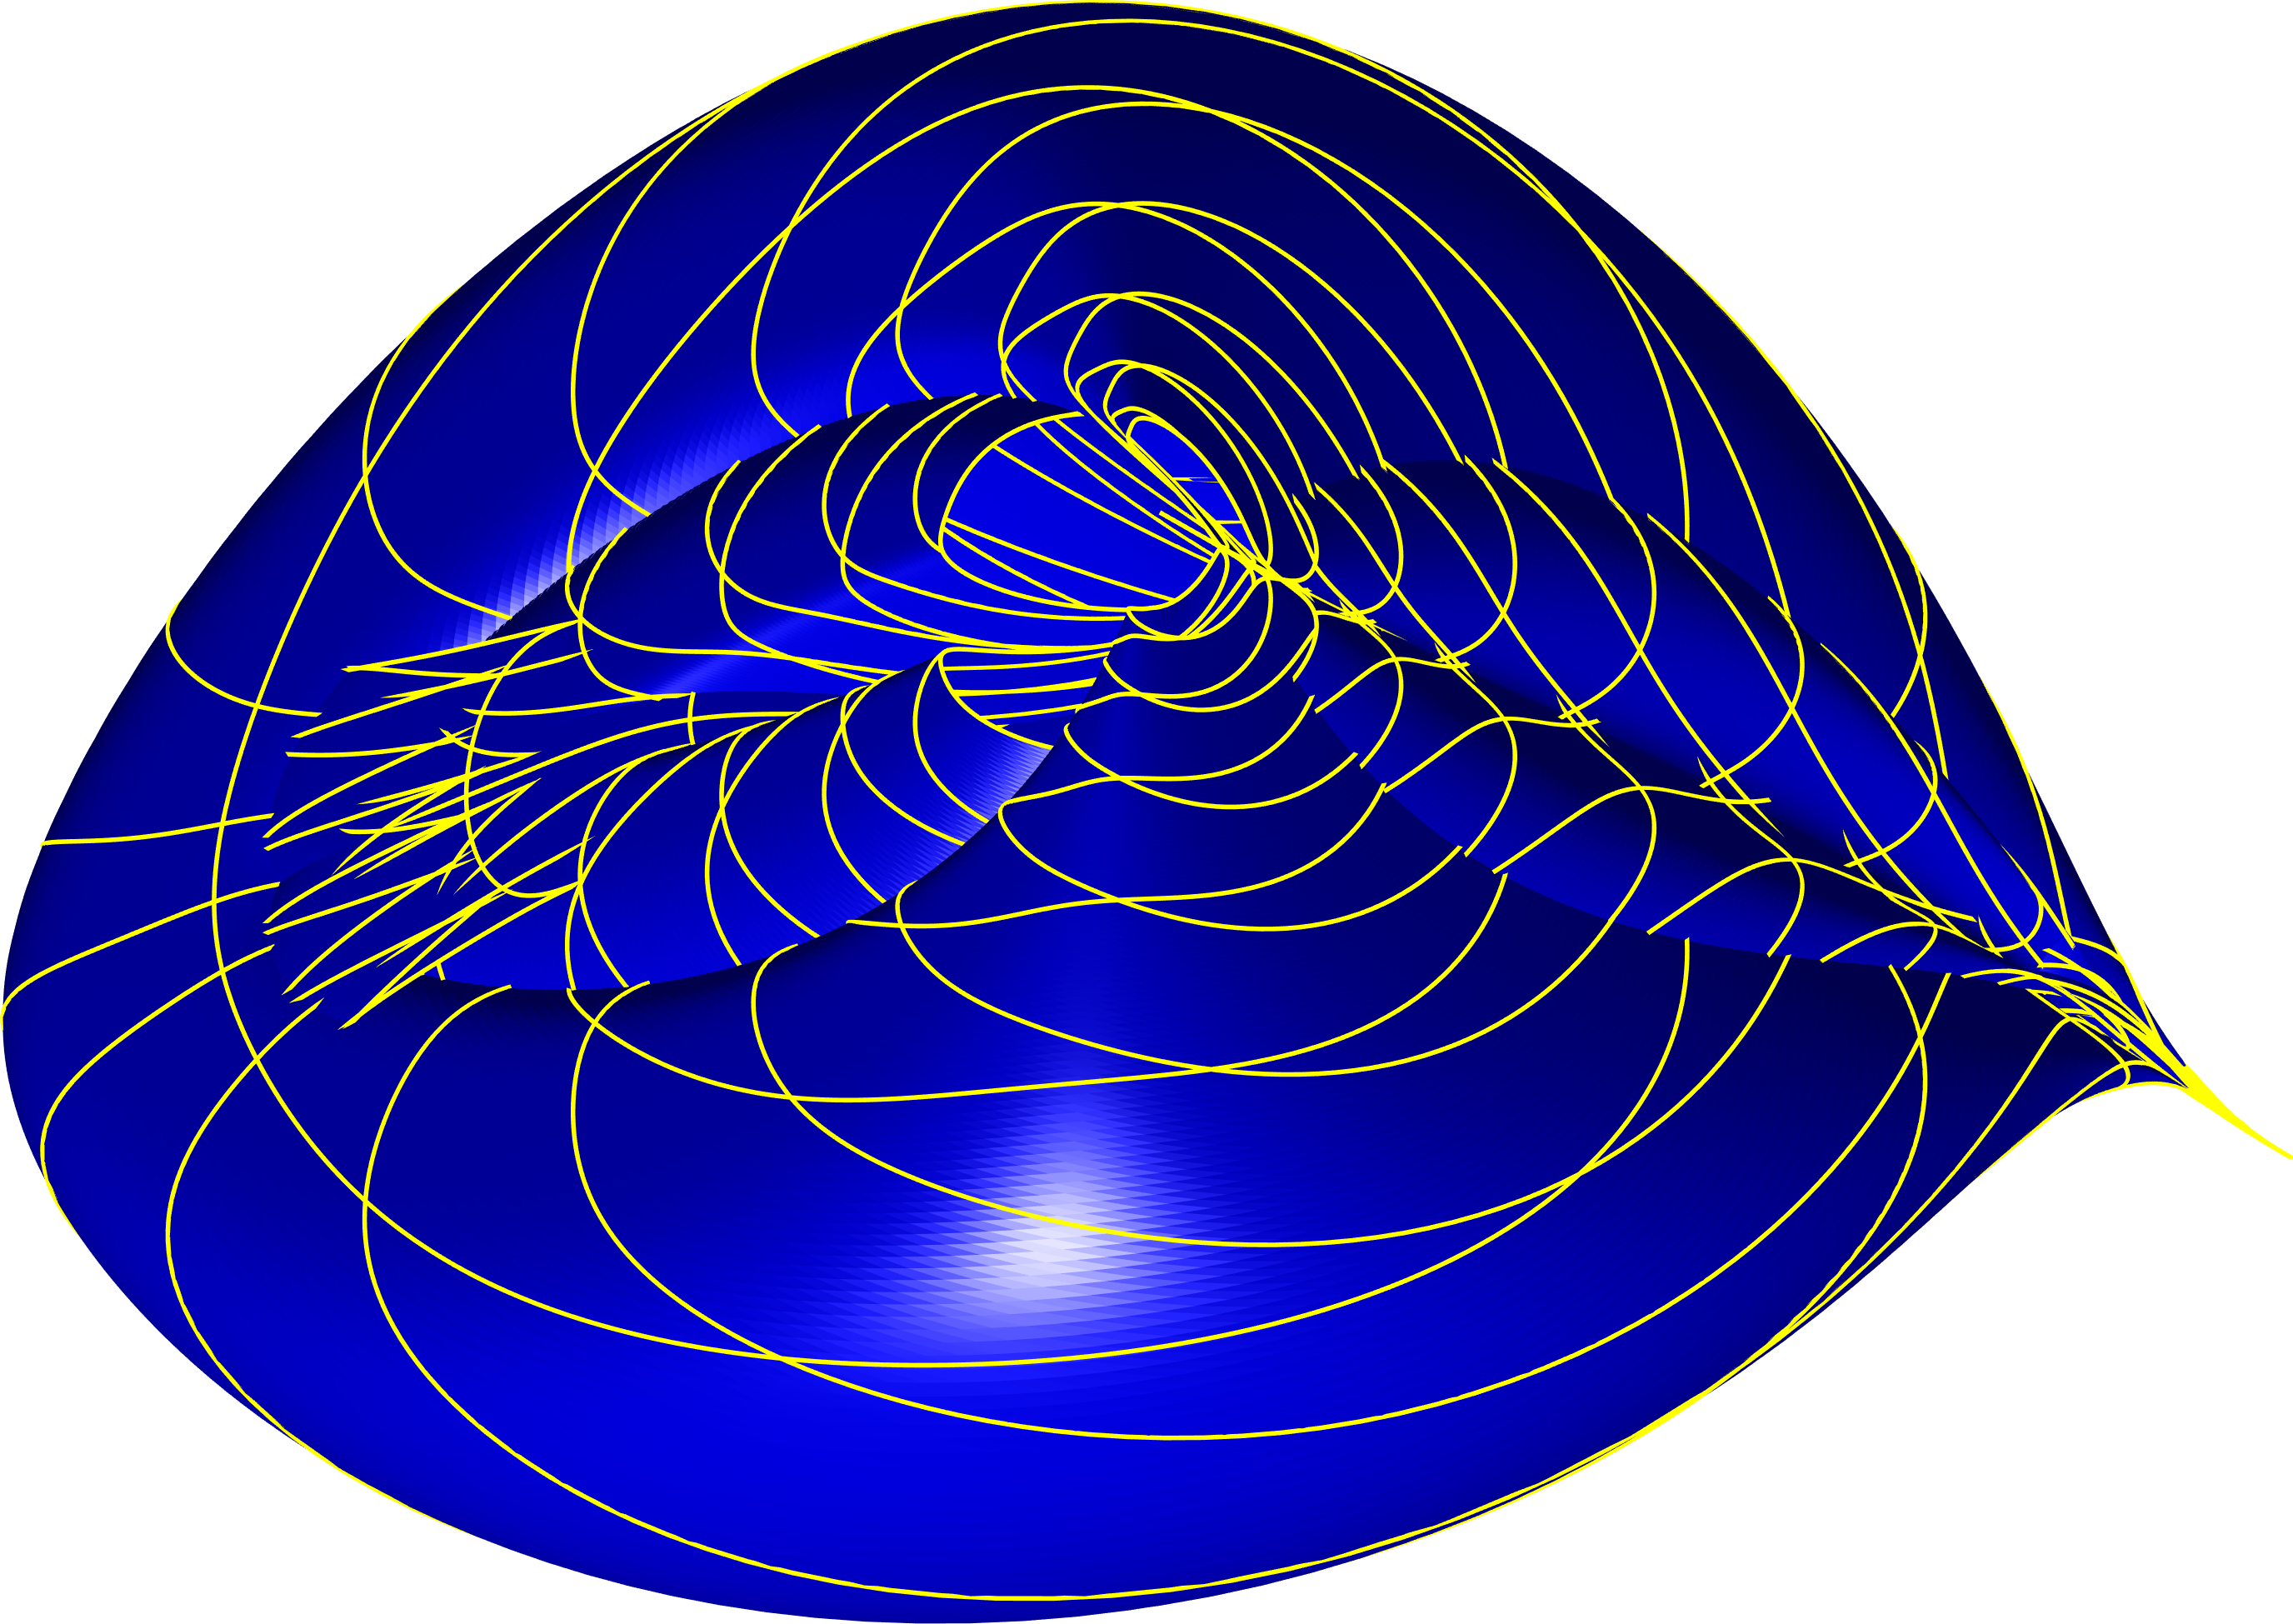
\includegraphics[width=.45\textwidth]{Figs/Mobius_signature.png}
\caption{A sample M\"obius Transform and 3D signature.}
\label{fig:mobius}
\end{figure}

\subsection{The Projective Group}

We consider the eight-dimensional group $\mathrm{PSL}(3,\R)$ acting on $\R^2$ by projective transformations, i.e., 
\begin{equation}
(x,y) \mapsto \left(\frac{a x + b y + j}{l + g x + h y}, \frac{c x + d y + k}{l+ g x + h y}\right).
\end{equation}

Requiring that $\bar f = f$ enables us to clear the translation coefficients, so $j=k=0$; for convenience we will also take $l=1$. This leaves 6 group parameters $(a,b,c,d,g,h)$ to be determined. For free action it is necessary to prolong the group action to 3rd derivatives of $f$. Since there are 9 derivatives of $f$ of order 1, 2, and 3, there will be at least 3 invariants.

The prolonged action is:
\begin{equation}
\arraycolsep=1.4pt
\label{eq:prolong}
%\rotatebox{90}{$
\left[
\begin{array}{c}
  \bar f_{\bar x} \\ \bar f_{\bar y} \\ \bar f_{\bar x \bar x} \\ \bar f_{\bar x \bar y} \\ \bar f_{\bar y \bar y} \\ \bar f_{\bar x \bar x \bar x} \\ \bar f_{\bar x \bar x \bar y} \\ \bar f_{\bar x \bar y \bar y} \\ \bar f_{ \bar y \bar y \bar y} 
 \end{array}
 \right]
 = 
\left[
\begin{array}{ccccccccc}
 a & c & 0 & 0 & 0 & 0 & 0 & 0 & 0 \\
 b & d & 0 & 0 & 0 & 0 & 0 & 0 & 0 \\
 -2 a g & -2 c g & a^2 & 2 a c & c^2 & 0 & 0 & 0 & 0 \\
 -b g-a h & -d g-c h & a b & b c+a d & c d & 0 & 0 & 0 & 0 \\
 -2 b h & -2 d h & b^2 & 2 b d & d^2 & 0 & 0 & 0 & 0 \\
 6 a g^2 & 6 c g^2 & -6 a^2 g & -12 a c g & -6 c^2 g & a^3 & 3 a^2 c & 3 a c^2 & c^3 \\
 2 g \alpha_1 & 2 g \beta_1 & -2 a \alpha_2 & -4 \delta_1 & -2 c \beta_2
   & a^2 b & a \gamma_1 & c \gamma_1 & c^2 d \\
 2 h \alpha_2 & 2 h \beta_2 & -2 b \alpha_1 & -4 \delta_2 & -2 d \beta_1
   & a b^2 & b \gamma_1 & d \gamma_2 & c d^2 \\
 6 b h^2 & 6 d h^2 & -6 b^2 h & -12 b d h & -6 d^2 h & b^3 & 3 b^2 d & 3 b d^2 & d^3 \\
\end{array}
\right]\left[
\begin{array}{c}
f_x \\ f_y \\ f_{xx} \\ f_{xy} \\ f_{yy} \\ f_{xxx} \\ f_{xxy} \\ f_{xyy} \\ f_{yyy} 
 \end{array}
 \right].%$}
 \end{equation}

\noindent where $\alpha_1 = b g + 2 a h, \alpha_2 = 2 b g + a h$, $\beta_1 = d g + 2 c h, \beta_2 = 2 d g + c h$, $\gamma_1 = b c + 2 a d, \gamma_2= 2 b c + a d$, and $\delta_1 = (b c g+a d g+a c h), \delta_2 = (b d g+b c h+a d h)$.
%\left[
%\begin{array}{ccccccccc}
 %a & c & 0 & 0 & 0 & 0 & 0 & 0 & 0 \\
 %b & d & 0 & 0 & 0 & 0 & 0 & 0 & 0 \\
 %-2 a g & -2 c g & a^2 & 2 a c & c^2 & 0 & 0 & 0 & 0 \\
 %-b g-a h & -d g-c h & a b & b c+a d & c d & 0 & 0 & 0 & 0 \\
 %-2 b h & -2 d h & b^2 & 2 b d & d^2 & 0 & 0 & 0 & 0 \\
 %6 a g^2 & 6 c g^2 & -6 a^2 g & -12 a c g & -6 c^2 g & a^3 & 3 a^2 c & 3 a c^2 & c^3 \\
 %2 g (b g+2 a h) & 2 g (d g+2 c h) & -2 a (2 b g+a h) & -4 (b c g+a d g+a c h) & -2 c (2 d
   %g+c h) & a^2 b & a (2 b c+a d) & c (b c+2 a d) & c^2 d \\
 %2 h (2 b g+a h) & 2 h (2 d g+c h) & -2 b (b g+2 a h) & -4 (b d g+b c h+a d h) & -2 d (d g+2
   %c h) & a b^2 & b (b c+2 a d) & d (2 b c+a d) & c d^2 \\
 %6 b h^2 & 6 d h^2 & -6 b^2 h & -12 b d h & -6 d^2 h & b^3 & 3 b^2 d & 3 b d^2 & d^3 \\
%\end{array}
%\right]

%%A direct calculation using (\ref{eq:prolong}) shows that the same transformation rule (\ref{eq:D}) holds for $\phi\in\mathrm{PSL}(3,\R)$.  That is, $D$ is a relative invariant of weight 2 of this action. 
%Both $D$ and $E$ will be useful quantities shortly, but note that, from (\ref{eq:D}), the sign of $D$ is invariant and therefore the choice of moving frame must depend on its sign. 

We begin by choosing the frames $\bar f_{\bar x} = 1$ and $\bar f_{\bar y}=  0$, which determine the group parameters $a = (1-c f_y)/f_x.$ and $b = -d f_y/f_x$. Direction substition then shows that $\bar f_{\bar y \bar y} = D d^2 / f_x^2$, where $D = f_{x}^2 f_{yy} + f_y^2 f_{xx} - 2 f_x f_y f_{xyy}$, which we saw earlier as an invariant of $A(2)$, which is a subgroup of $\mathrm{PSL}(3,\R)$. Note that $D$ and $\bar f_{\bar y \bar y}$ have the same sign; in what follows we assume that $D>0$ (if it is negative, relatively little changes in the following derivation) and choose the frame $\bar f_{ \bar y \bar y} = 1$, so that $d = f_x/D^{1/2}.$

The frame $\bar f_{ \bar y \bar y \bar y} = 0$ determines the group parameter $ h = \frac{d(f_{yyy}f_x^3 - 3 f_x^2 f_y f_{xyy} + 3 f_x f_y^2 f_{xxy} - f_y^3 f_{xxx})}{6 f_x D},$ while $\bar f_{ \bar x \bar y \bar y}=0$ provides $ c = \frac{h f_x^2}{d D} - \frac{f_x f_{xy} - f_y f_{xx}}{D}$, and $\bar f_{ \bar x \bar x}=0$ gives $ g = \frac{1}{2 f_x^2}(f_{xx} + 2 c ( f_x f_{xy} - f_y f_{xx} ) + c^2 D).$ In fact, the denominator of the expression for $h$ was another invariant of $A(2)$; we label it $E$ for convenience.

%\begin{equation}
%E := f_{yyy}f_x^3 - 3 f_{xyy}f_x f_y^2 + 3 f_{xxy}f_x^2 f_y - f_{xxx}f_y^3.
%\end{equation}

Having determined the frame, any function of the remaining derivatives $\bar f_{ \bar x \bar x \bar x}$, $\bar f_{ \bar x \bar x \bar y}$, and $\bar f_{ \bar y \bar y \bar y}$, as given in Equation~(\ref{eq:prolong}), provides invariants. We choose: $$ (f_{xxx}, f_{xxy}^2, f_{xyy})=\left(\frac{J_1}{D^6},\frac{J_2}{D^9},\frac{J_3}{D^3}\right)$$, where (with $P_n$ denoting a polynomial of degree $n$):
$$ J_1 = E^4 + D P_{13},\quad J_2 = (E^3 + D P_9)^2,\quad J_3=E^2 -12 D P_5.$$

The $J_i$ are polynomials of degree 16, 24, and 8, respectively, and are extremely complicated when written out explicitly. They do have one benefit, though, which is that they  all have denominators given by integer powers of $D$, resolving the ambiguity caused by the sign of $D$. Therefore, $$ (D^{18}, J_1^3, J_2^2, J_3^6)$$ are all relative invariants of weight 36, and so projecting any subset of them of them to a sphere yields a third-order invariant signature.

$J$ vanishes on generic images: $J=0$ when $D=E=0$, which is a codimension 0 phenomenon for images. In particular, $D=E=0$ at critical points. However, these signatures can be simplified and made more robust. Their structure suggests considering the combination $J_1 - J_3^2$, which obeys:
$$J_1 - J_3^2 = 144 D^4 P_4.$$

As $J_1/D^6$ and $J_3/D^3$ are invariant, so is $P_4/D^2$. 
Moreover, the numerator of this new invariant does not vanish at critical points.  It has the structure:
$$P_4 = -4(\det f_{ij})^2 + Q_4,$$
where $Q_4$ is a polynomial of degree 4 that vanishes when $f_x=f_y=0$. Hence, the relative invariant of weight 12:
$$ (D^6, P_4^3, (E^2-12D P_5)^2)$$
can be projected to $S^2$, yielding a projective invariant of images that is singular only when $D=E=P_4=0$, which is a codimension 1 phenomenon, since  $D=E=0\Rightarrow P_4=0$. In particular, at critical points it tends to:
$(0, (2\det f_{ij})^6, 0),$ and hence critical points with $\det f_{ij}\ne 0$ have signature value $(0,1,0)$.
Including $J_2$ provides a 4-dimensional signature set, but does not increase the codimension of the set of bad images.

\todo[inline]{Is this useful? Is it what we actually use? If so, fix the names...}
For completeness we write out the invariant signature we use explicitly:

$Q_4=4 f_x  f_{xy} ^2 f_{xyy}  - 
f_x ^2 f_{xyy} ^2 - 
 2 f_{yyy}  f_x  f_{xy}  f_{xx}  + 
 2 f_{yy}  f_x  f_{xyy}  f_{xx}  - 
 6 f_{y}  f_{xy}  f_{xyy}  f_{xx}  + 
 2 f_{y}  f_{yyy}  f_{xx} ^2 + 
 f_{yyy}  f_x ^2 f_{xxy}  - 
 6 f_{yy}  f_x  f_{xy}  f_{xxy}  + 
 4 f_{y}  f_{xy} ^2 f_{xxy}  + 
 f_{y}  f_x  f_{xyy}  f_{xxy}  + 
 2 f_{y}  f_{yy}  f_{xx}  f_{xxy}  - 
 f_{y} ^2 f_{xxy} ^2 + 
 2 f_{yy} ^2 f_x  f_{xxx}  - 
 f_{y}  f_{yyy}  f_x  f_{xxx}  - 
 2 f_{y}  f_{yy}  f_{xy}  f_{xxx}  + f_{y} ^2 f_{xyy}  f_{xxx}, $
 
$P_5=f_{yyy}  f_{x} ^3 f_{xy}  - 
f_{yy}  f_{x} ^2 f_{xy} ^2 + 
 2 f_{y}  f_{x}  f_{xy} ^3 - 
 f_{yy}  f_{x} ^3 f_{xyy}  - 
 f_{y}  f_{x} ^2 f_{xy}  f_{xyy}  + 
 f_{yy} ^2 f_{x} ^2 f_{xx}  - 
 f_{y}  f_{yyy}  f_{x} ^2 f_{xx}  - 
 2 f_{y}  f_{yy}  f_{x}  f_{xy}  f_{xx}  - 
 f_{y} ^2 f_{xy} ^2 f_{xx}  + 
 2 f_{y} ^2 f_{x}  f_{xyy}  f_{xx}  + 
 f_{y} ^2 f_{yy}  f_{xx} ^2 + 
 2 f_{y}  f_{yy}  f_{x} ^2 f_{xxy}  - 
 f_{y} ^2 f_{x}  f_{xy}  f_{xxy}  - 
 f_{y} ^3 f_{xx}  f_{xxy}  - 
 f_{y} ^2 f_{yy}  f_{x}  f_{xxx}  + 
 f_{y} ^3 f_{xy}  f_{xxx}. $
 
Further invariants can be found by noting that, for any planar transformation group and any two invariants
$I^1$ and $I^2$, $\nabla I^1 \times \nabla I^2$ is a relative invariant of weight 1; that is:
$$\nabla I^1 \times \nabla I^2\mapsto (\det \phi')(\nabla I^1 \times \nabla I^2).$$
Applying this operation to $f$ and the four third-order invariants yields $5\cdot4/2=10$ fourth-order invariants.

\begin{figure}
\centering
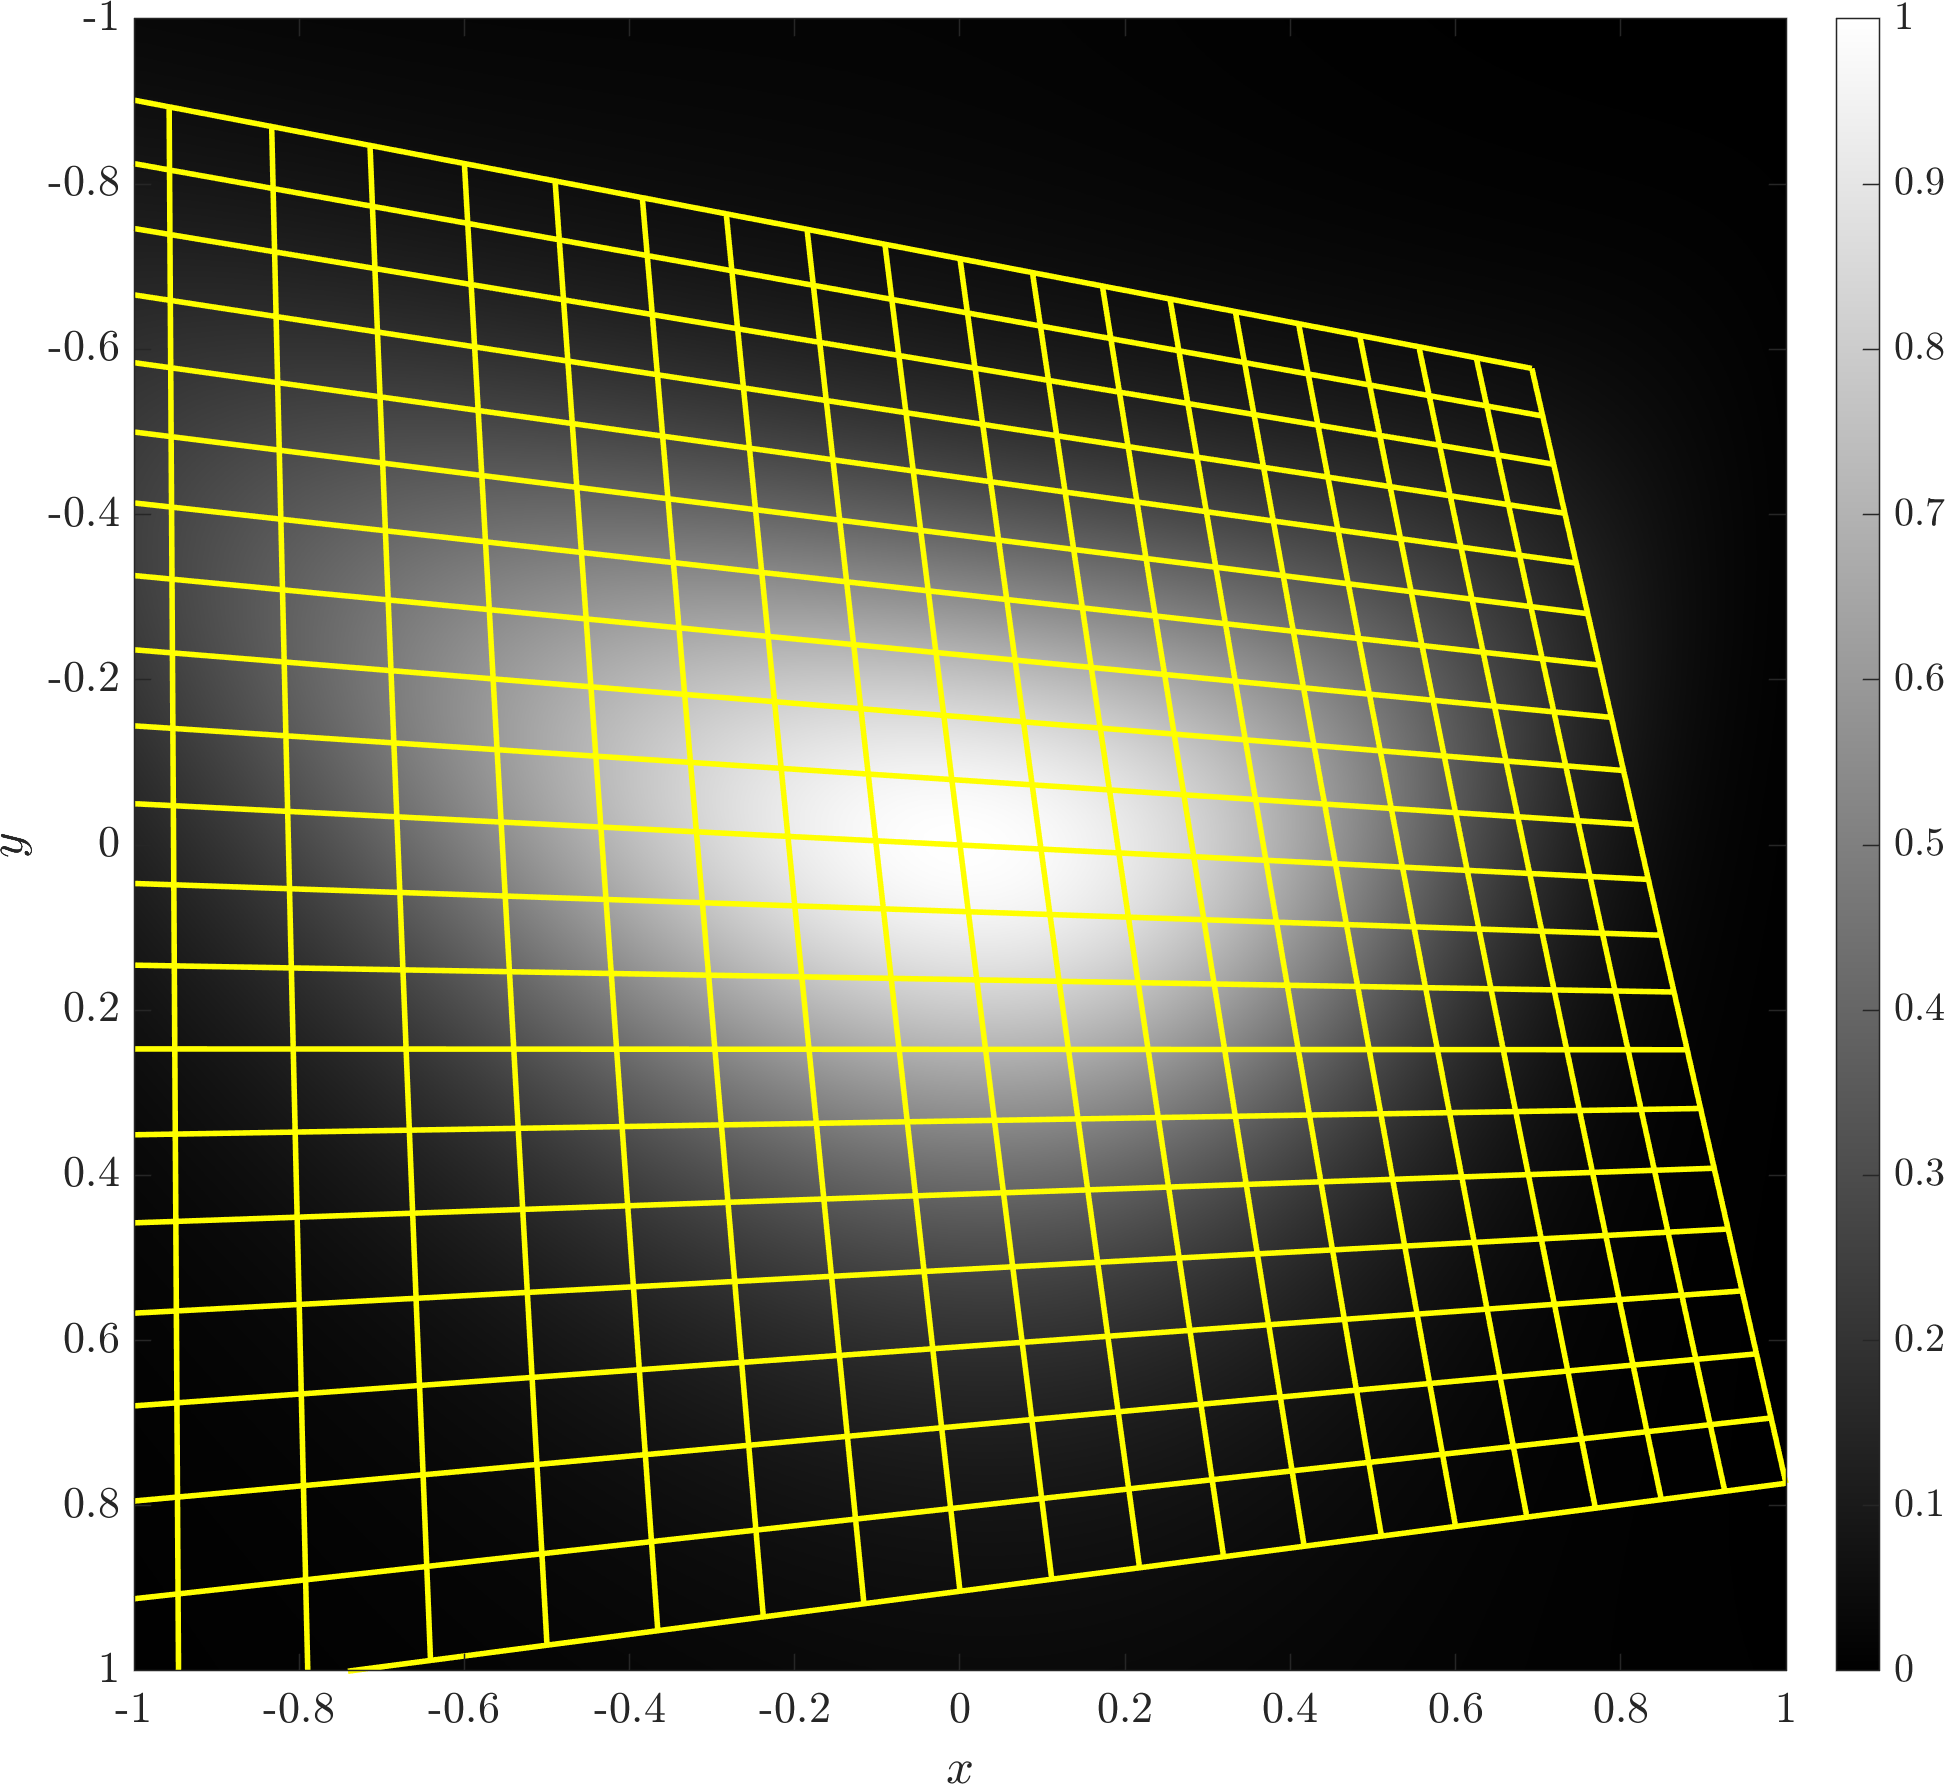
\includegraphics[width=.45\textwidth]{Figs/f_transformed_PSL3R.png}
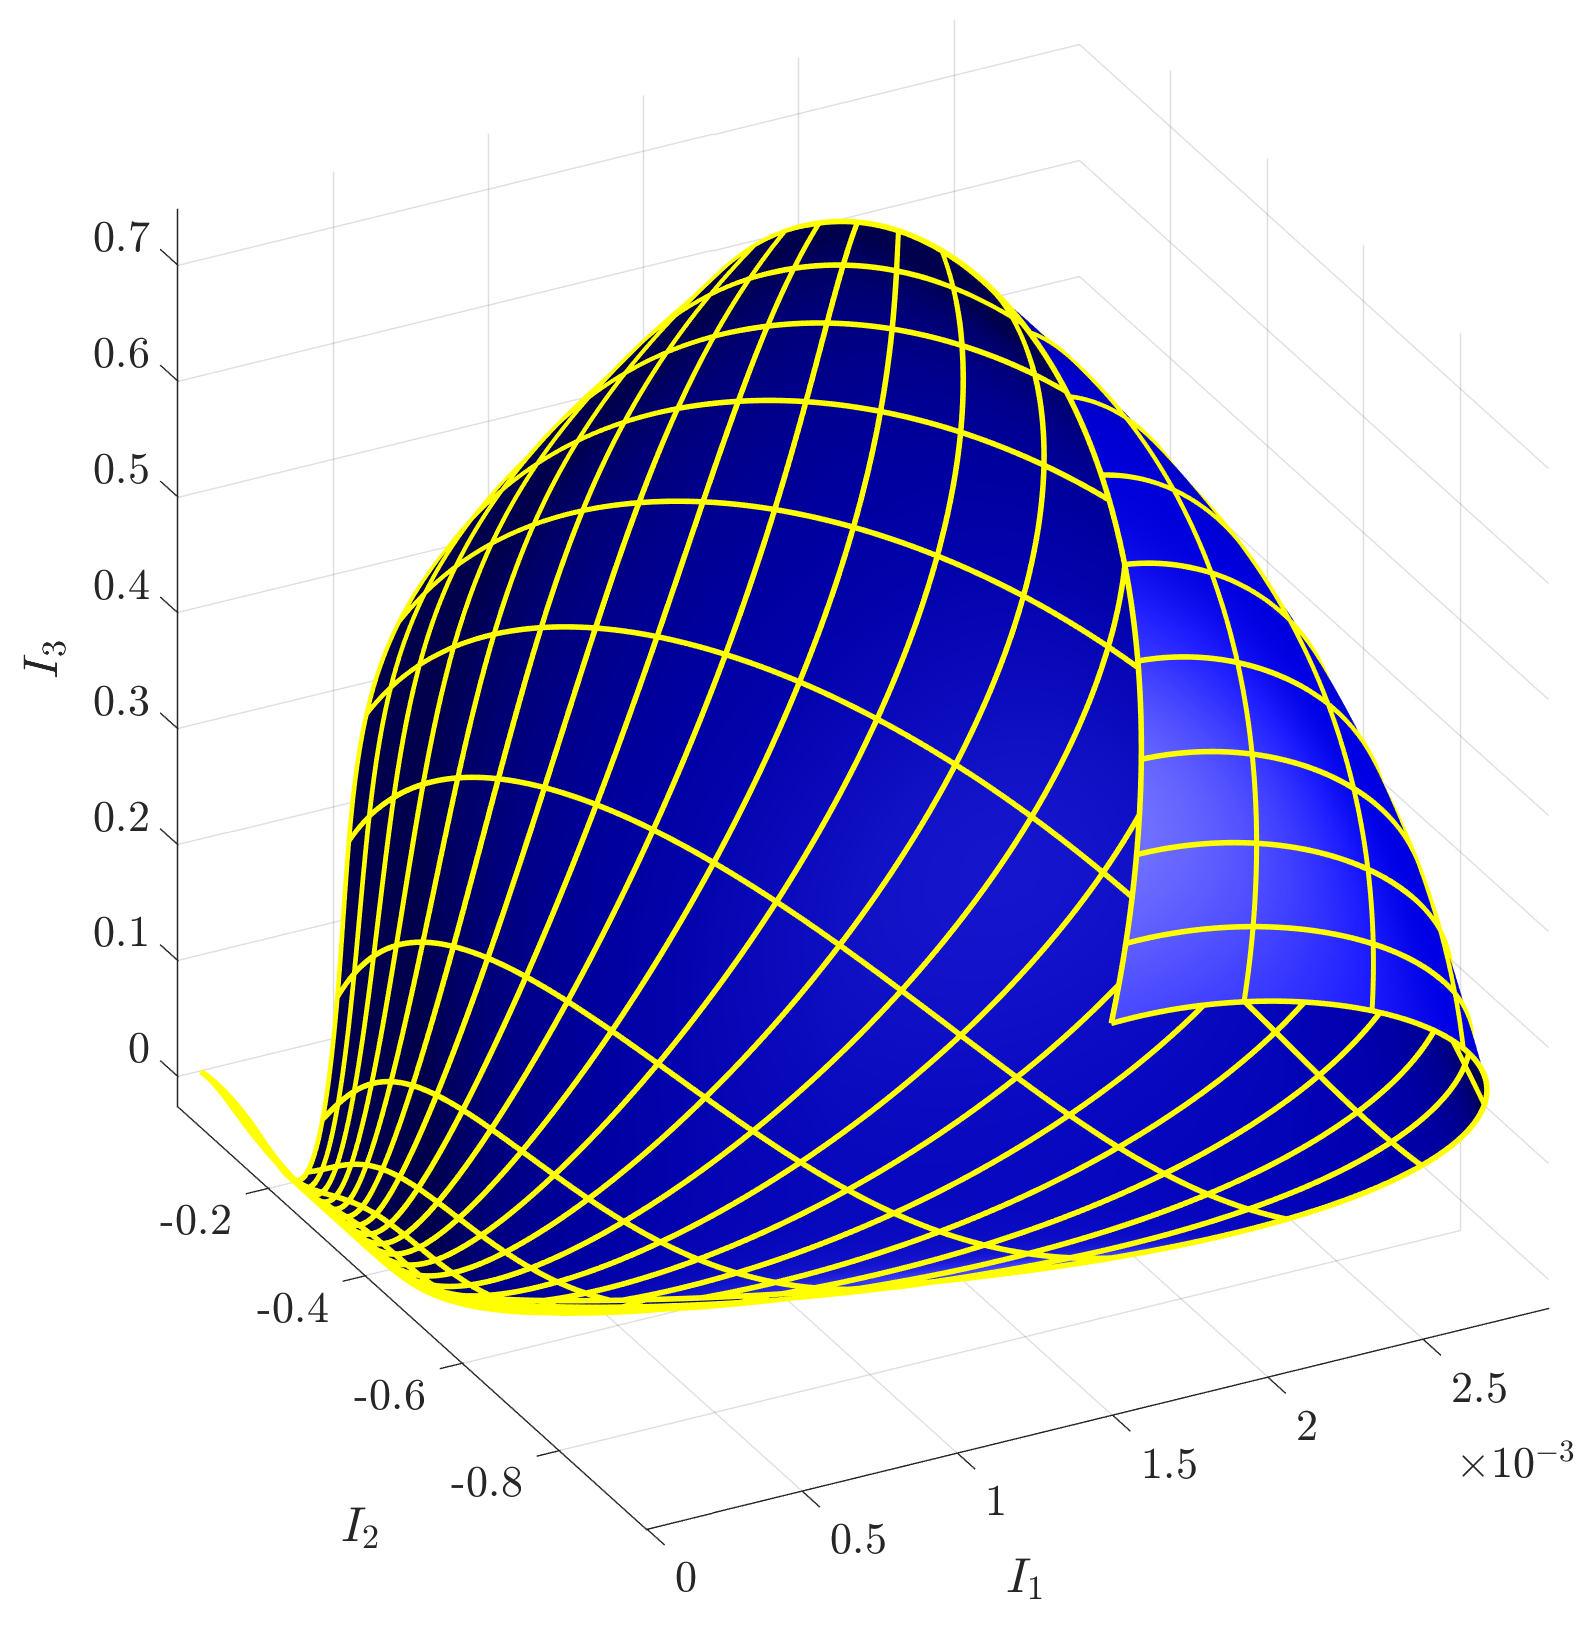
\includegraphics[width=.45\textwidth]{Figs/PSL3R_signature.png}
\caption{A sample $PSL(3,\mathbb{R})$ Transform and 3D signature.}
\label{fig:PSL3R}
\end{figure}

\subsection{Conformal Diffeomorphisms $\mathbf{Diff}_{\mathbf{con}}$}

The group of conformal diffeomorphisms is the subgroup of diffeomorphisms that are angle-preserving, i.e.,

\begin{equation}
\angle (u,v) = \angle (D \phi(x) . u, D \phi(x).v)
\end{equation}

\noindent where $\angle(u, v)$ denotes the angle between tangent vectors
$u$ and $v$ based at $x \in \mathbb{R}^2$, $\phi \in \textrm{Diff}$ and $D$
represents the Jacobian. The group is infinite-dimensional, but still small
enough that images have local differential invariants. 

The conformal diffeomorphisms provides a particularly nice example of the
moving frame method. Because the group is infinite dimensional, we need to
prolong the group action to the infinite jet space $J^{\infty}$ with
elements of the form $(x, y, f, f_x, f_y, f_{xx}, f_{xy}, f_{yy}, \ldots)$.
Recall the moving frame produces a conformal map $\psi$ for each element of
$J^\infty$ that maps it to a suitably chosen cross section. 

It's convenient to work in the complex variable $z = x + iy$. Without loss of
generality, we can assume $x = y = 0$. We begin the construction of our
cross section by choosing $\bar{x} = \bar{y} = 0$. Then, $\psi^{-1}$ 
can be represented locally by a Taylor series of the form
\begin{equation*}
    z = \psi^{-1}(\bar{z}) = c_1 \bar{z} + c_2 \bar{z}^2 + c_3\bar{z}^3 + \cdots
\end{equation*}
where $c_k = a_k + ib_k, k = 1, 2, \ldots$. We solve for the parameters
$a_k, b_k$ in stages.  To find $c_1 = a_1 + i b_1$ we need two constraints.
Differentiating $f(x, y) = \bar{f}(\bar{x}, \bar{y})$ and substituting in
our existing cross section constraints $\bar{x} = \bar{y} = 0$ gives
\begin{align*}
    \bar{f}_{\bar{x}} = f_x x_{\bar{x}} + f_y y_{\bar{x}} &= a_1 f_x + b_1
    f_y, \\
    \bar{f}_{\bar{y}} = f_x x_{\bar{y}} + f_y y_{\bar{y}} &= -b_1 f_x + a_1
    f_y. 
\end{align*}
Note that $\bar{x} = \bar{y} = 0$ removes all higher order derivatives from
the cross section equation. Adding two extra constraints to the cross
section, $\bar{f}_{\bar{x}} = 1, \bar{f}_{\bar{y}} = 0$, this system is readily
solved to give 
\begin{equation*}
    \begin{aligned}
        a_1 &= f_x / (f_x^2 + f_y^2), &  b_1 &= f_y / (f_x^2 + f_y^2).
    \end{aligned}
\end{equation*}
We then repeat the process, this time using the second derivative
computations. This time, there are two new parameters, $a_2, b_2$, to solve
for, but there are three derivatives. We use the cross section equations
$\bar{f}_{\bar{x}\bar{x}} = 0, \bar{f}_{\bar{x}\bar{y}} = 0$ to solve for
$a_2$ and $b_2$, the remaining derivative $\bar{f}_{\bar{y}\bar{y}}$ is then the
sole second-order invariant, which we also saw for the M\"obius group: 
\begin{equation*}
    \bar{f}_{\bar{y}\bar{y}} = \frac{f_{xx} + f_{yy}}{f_x^2 + f_y^2}.
\end{equation*}
Continuing in this way, at derivative order $n$ two real group parameters
enter: $a_n$ and $b_n$. There are $n+1$ independent derivatives of $f$ of
order $n$, so there must be $n-1$ new independent invariants at each order.
Hence at third order there are two more invariants, using the constraints
$\bar{f}_{\bar{x}\bar{x}\bar{x}} = 0, \bar{f}_{\bar{x}\bar{x}\bar{y}} = 0$,
the remaining derivatives are invariant:
\begin{align*}
    \bar{f}_{\bar{x}\bar{y}\bar{y}} &= \frac{f_y^3f_{yyy} + f_x^2f_yf_{yyy}
            -2f_y^2f_{yy}^2 - 2f_{xx}f_y^2f_{yy} -
            4f_xf_{xy}f_yf_{yy} - 2f_x^2 f_{xx}f_{yy} + f_{xxy}f_y^3 +
            f_x^2 f_{xxy}f_y - 4 f_x f_{xy} f_{xx} f_y + f_x^3 f_{xxx} -
        2f_x^2 f_{xx}^2 + f_x^3 f_{xyy}}{(f_x^2 + f_y^2)^3} \\
        \bar{f}_{\bar{y}\bar{y}\bar{y}} &= \frac{f_xf_y^2f_{yyy} +
        f_x^3f_{yyy} - 2f_x f_y f_{yy}^2 + 2f_{xy}f_y^2f_{yy} -
    2f_x^2f_{xy}f_{yy} - f_{xxx}f_y^3 - f_{xyy}f_y^3 + f_xf_{xxy}f_y^2 +
2f_{xy}f_{xx}f_y^2 - f_x^2 f_{xxx} f_y + 2f_xf_{xx}^2 f_y - f_x^2 f_{xyy}
f_y + f_x^3 f_{xxy} - 2f_x^2 f_{xy} f_{xx} }{(f_x^2 + f_y^2)^3 }
\end{align*}

%However, we first note that the M\"obius action is locally identical to the full conformal group up to and including second order. Therefore, there are no new conformal invariants, apart from the M\"obius ones, up to second order. It is possible to identify some invariants via direct calculation using the defining geometric properties of the conformal group.

%At second order, we first consider the action of conformal maps on the Euclidean invariants $f_i f_i$ and $f_{ii}$.

%Let $\psi := \varphi^{-1}$. For any diffeomorphism, the derivatives of $f$ transform as
%$$f_i \mapsto f_j \psi^j_i$$
%and
%$$f_{ij} \mapsto f_{kl} \psi^k_i\psi^l_j + f_{k}\psi^k_{ij}.$$
%Therefore the Laplacian of $f$ transforms as
%$$ f_{ii} \mapsto f_{kl} \psi^k_i \psi^l_i + f_k \psi^k_{ii}.$$
%When $\psi=u + i v$ is conformal, $\psi_{k,ii}=0$ because the components of conformal maps are harmonic functions,
%and the Cauchy-Riemann equations give $\psi_{k,i}\psi_{l,i} = (u_x^2 + u_y^2)\delta_{kl}$. Therefore,
%$$ f_{ii} \mapsto f_{ii}(u_x^2+u_y^2).$$
%Here $u_x^2+u_y^2=\det\psi^k_i$ is the local scaling factor of the transformation.
%Note also that
%$$f_i f_i \mapsto f_k f_l \psi_{k,i} \psi_{l,i} = f_k f_k (u_x^2 + u_y^2).$$
%That is, $f_{ii}$ and $f_i f_i$ are both relative invariants of weight 2, while $f_{ii}/(f_i f_i)$ is a conformal invariant, as we saw for the M\"obius group. By itself, it is not useful for images as it is singular at critical points of $f$.


%The transformation of 1st derivatives is more clearly written in complex variables as $$ f_x + i f_y \mapsto a_1 (f_x + i f_y).$$ Given any two real invariants $g,h$, the real and imaginary parts of $(g_x+i g_y)(h_x-i h_y)$ are relative invariants of weight 2. This generates the required two invariants of order 3. (We have repeated and confirmed this calculation using the method of moving frames.) 

\todo[inline]{Fix up this bit to be correct and complete for what we do}
Specifically, let $J_1 = f_i f_i$ and  $J_2 = f_{ii}$, so that  $g = J_2/J_1$ is invariant.  We want to work with polynomials, so we clear denominators and let $J_3+iJ_4 = J_1^2 (g_x + i g_y)  (f_x - i f_y)$. $J_3$ and $J_4$ are a differential polynomials of $f$ of degree 4 and order 3, and are relative invariants of weight 6. They can be written explicitly as functions of the basic invariants of $SE(2)$ as
$$J_3 = f_k f_k f_{iij}f_j - 2 f_{ii} f_{jk} f_j f_k$$
and (writing $a_i\times b_i$ for $a_1 b_2 - b_2 a_1$)
$$ J_4 = f_k f_k f_{iij}\times f_j - 2 f_{ii} f_{jk} f_k\times f_j.$$
Under conformal maps we have
$$ (J_1,J_2,J_3,J_4) \mapsto (|a_1|^2 J_1, |a_1|^2 J_2, |a_1|^6 J_3,|a_1|^6 J_4).$$

Therefore, projecting $(J_1^3,J_2^3,J_3)$ to the unit sphere, together with $f$ itself, provides a conformal signature set in $\R\times S^2$. It is continuous at all $(x,y)$ such that $J_1$, $J_2$, and $J_3$ are not simultaneously equal to zero.  Now $J_1=0$ implies $f_1=f_2=0$, and $J_2=0$ implies $f_{ii}=0$, but these together imply $J_3=0$. Thus the signature set is discontinuous when $f_1=f_2=f_{ii}=0$, a codimension-1 phenomenon for images.

Similarly, projecting $(J_1^3,J_2^3,J_3,J_4)$ to the unit sphere, together with $f$ itself, provides a conformal signature set in $\R\times S^3$. This is also singular when $f_1=f_2=f_{ii}=0$. These singularities are not removable. A typical image near a `bad' point takes the form $f = a(x^2-y^2) + b x y + c x^3 + d x^2 y + e x y^2 + g y^3$.  For such an $f$, $(J_1^3,J_2^3,J_3,J_4)=\mathcal{O}(x^6,x^3,x^3,x^3)$.  The cubic forms always change sign and do not generically lead to a well-defined direction as $(x,y)\to(0,0)$. 

\subsection{Volume-Preserving Diffeomorphisms $\mathbf{Diff_{vol}}$}

The subgroup of volume-preserving diffeomorphisms are those diffeomorphisms that preserve the volume form, which in 2D is actually the area form. They can be defined by one function of two variables, the generating function $S$; one possibility is $S(x,y')$ where $(x,y)\mapsto(x',y')$ according to
$$ x'=\frac{\partial S}{\partial y'},\quad y = \frac{\partial S}{\partial x}.$$

Consider expanding $S$ in Taylor series. The linear terms in the map are determined from the quadratic terms in $S$, which contain 3 group parameters, and act on 2 coordinates, $f_x$ and $f_y$.  The quadratic terms in the map are determined from the cubic terms in $S$, which contain 4 group parameters, and act on 3 coordinates, $f_{xx}$, $f_{xy}$, and $f_{yy}$. At order $n$ we have $n+2$ new group parameters acting on $n+1$ coordinates. Thus, barring some exceptional behaviour in the action, we do not expect any invariants at generic points.

This can be confirmed by considering a small image patch with $f(x,y)=x.$ Let $v=\psi_y\partial/\partial_x - \psi_x\partial/\partial_y$ be the generator of an area-preserving map. The image $f$ transforms to $x + \varepsilon \psi_y(x,y)$ which (by choosing $\psi$ appropriately) can be any function close to $x$.

At nongeneric points, there can be invariants. For example, the area enclosed in any level set of $f$ is invariant. At minima or maxima of $f$, this will lead to invariants expressed in terms of the derivatives of $f$.

\section{Colour Images}\label{sec:colour}

The formulation we provided in the introduction considered $k$ channels of information. So far we have considered only greyscale images ($k=1$), but most real images are three-channel colour (RBG), and multi-spectral images can have hundreds of channels of measurement. It is therefore natural to consider whether this information is useful for the computation of invariants. 

The hope is that by constructing invariants using different colour channels, fewer derivatives are needed: for $k$ colours, signature sets of dimension up to $k + k(k+1)/2$ can be chosen from the invariants $f^i$ and $f^i_m f^j_m$ for $i,j=1,\dots, k$. However, the situation is more complicated that it first appears because the information in the channels is not independent: colour is built by the intensities in the three channels, and so there is correlation between them. We briefly sketch some possibilities for some of the groups that we have considered earlier, but note that the correlation means that the invariant signatures identified next are na\"ive, and should be viewed as best-case scenarios. 

\begin{description}
\item[$E(2)$]
Considering $E(2)$, for $k\ge 2$, first derivatives suffice. However, note that for $k\ge 3$ the three-dimensional signature $(f^1,f^2,f^3)$ is invariant under all local planar diffeomorphisms and so a higher-dimensional signature, involving at least first derivatives, is required.
\item[$SA(2)$]
For $SA(2)$, one can take transvectants of any components of $f$ to get invariants. For $k=2$ colours, there is only one  invariant formed from first derivatives, namely $((f^1)',(f^2)')_x = f^1_x f^2_y - f^1_y f^2_x$ (the Poisson bracket $\{f^1,f^2\}$). So again two derivatives are necessary, even for a 3-dimensional signature.

For $k\ge 3$ colours there are plenty of invariants formed from first derivatives, namely $\nabla f^i \times \nabla f^j$ for $i<j$. However, these are all invariant under the bigger group $\mathrm{Diff}_{\mathrm{vol}}$ of local volume-preserving diffeomorphisms, and so the Poisson brackets cannot form a complete invariant for $SA(2)$: two derivatives are always needed no matter how many colours we have. The relation $SA(2)\subset \mathrm{Diff}_{\mathrm{vol}}$ acts an obstruction to $SA(2)$, an instance of the phenomenon of hidden symmetry.
\item[$A(2)$]
The same problem occurs with $A(2)$. There are plenty of invariants formed from two derivatives: already 9 when $k=2$. However, as with $SA(2)$, we can never get away with one derivative because all the first-derivative invariants, such as $\{f^1,f^2\}/\{f^1,f^3\}$, are also invariant under $\mathrm{Diff}_{\mathrm{vol}}$ (even though $A(2)$ is not even a subgroup of $\mathrm{Diff}_{\mathrm{vo}l}$).
\item[$PSL(2,\mathbb{C})$]
Recall that M\"obius and conformal transformations cannot be distinguished by their action on second derivatives. Therefore at least three derivatives are needed, no matter how many colours we have. We can use, for example, the invariants arising from the curvature of the level sets of each colour. Replacing the relative invariant $\|\nabla f\|^2$ by $\sum_{j=1}^k \|\nabla f^j\|^2$, and $f_{ii}$ by $\sum_{j=1}^k (f^j_{ii})^2$, increases the codimension of the singular images from 1 to $3k-2$.
\item[$PSL(3,\mathbb{R})$]
In $PSL(3, \mathbb{R})$ for $2$-colour images, there are three second-order relative invariants of weight 2, namely $(D_1,D_2,(\nabla f^1\times \nabla f^2)^2)$. Together with $(f^1,f^2)$, these yield a 4-dimensional $\mathbb{R}^2\times S^2$-valued signature using only second derivatives. With $k>2$ colours there are many more second-order invariants; however, as the action of the projective group on first derivatives is indistinguishable from that of the full diffeomorphism group, it is not possible to have a first-order signature that distinguishes projectively-related images from diffeomorphically-related ones.
\item[$\mathrm{Diff}_{\mathrm{vol}}$]
When $k\ge 2$ in $\mathrm{Diff}_{\mathrm{vol}}$ there are $k(k-1)/2$ first-order invariants $ \nabla f^i \times \nabla f^j$.  We consider the case $k=2$ and the 3-dimensional signature $$ (f^1,f^2, \nabla f^1 \times \nabla f^2).$$ This signature determines (generically and locally) the image up to an area-preserving map.  We have seen that we can generically choose the area-preserving map so that $f^1=x$, and we assume that this has been done. The remaining freedom is that of the area-preserving maps that preserve $x$: these are the shears $y\mapsto y + g(x)$. The signature for each fixed $x$ now gives $(f^2,f^2_y)$. This is the standard signature curve for the group of translations in $y$. Thus, $f^2$ is determined by the signature up to a translation in $y$, i.e., an area-preserving map.
\item[$\mathrm{Diff}_{\mathrm{con}}$]
For the infinite-dimensional group $\mathrm{Diff}_{\mathrm{con}}$, first-order signature sets are possible for $k \ge 2$ colours. They are formed from the relative invariants $(f^j_1 + i f^j_2)(f^m_1 - i f^m_2)$ of weight 2. We illustrate this using the Hopf fibration for $k=2$. The weight 2 relative invariant $$J = (2(f^1_1 + i f^1_2)(f^2_1 - i f^2_2), ||\nabla f^1\|^2 - \|\nabla f^2\|^2)$$ obeys $\|J\|^2 = \|\nabla f^1\|^2 + \|\nabla f^2\|^2$, hence projecting to the unit sphere shows that $(f^1,f^2,J/\|J\|)$ provides a 4-dimensional signature set that is singular only when $\nabla f^1 = \nabla f^2 = 0$, a codimension 2 phenomenon for images.
\item[$\mathrm{Diff}$]
\todo{Move this one out}
In the full diffeomorphism group there are no differential invariants using 1 or 2 colours. For example, with $k=2$, for generic $f^1$, $f^2$ we can choose a diffeomorphism (i.e., choose local coordinates) so that $f^1=x$ and $f^2=y$. We therefore take $k\ge 3$. This provides the first-order relative invariants of weight 1 $\nabla f^i\times \nabla f^j$, and hence a first-order signature. However, a zeroth-order signature set is possible: $(f^1,\dots,f^k)$. This is the image of the image. It is (locally and generically) complete. We can choose coordinates so that $f^1=x$ and $f^2=y$; then the signature locally determines $f^3,\dots,f^k$ as functions of $f^1$ and $f^2$, i.e., the image.
\end{description}



\section{Conclusions}

\todo[inline]{Number of derivatives}
\todo[inline]{Noise; integral invariants, Fourier}
\todo[inline]{Is there a general theory - syzygy??}
\todo[inline]{Difficulties of a practical implementation}

\begin{table}[h]
\begin{center}
\begin{tabular}{| l | c c c |}
\hline
\# derivs. & $k=1$ & $k=2$ & $k=3$ \\
\hline
SE(2) & 2 &1 & 1 \\
E(2) & 2 & 1 & 1 \\
Sim(2) & 2 & 1 & 1 \\
SA(2) & 2 & 2 & 2 \\
A(2) & 3 & 2 & 2 \\
$\mathrm{PSL}(2,\mathbb{C})$ & 3 & 3 & 3 \\
$\mathrm{PSL}(3,\R)$ & 3 & 2 & 2 \\
$\mathrm{Diff}_{\mathrm{vol}}$ & -- & 1 & 1 \\
$\mathrm{Diff}_{\mathrm{con}}$ & 3 & 1 & 1 \\
$\mathrm{Diff}$ & -- & -- & 0 \\
\hline
\end{tabular}
\caption{Number of derivatives of $f$ needed to construct a differential invariant signature of $f$ as a function of the group $\mathcal{G}$ and the number of colours $k$ of $f$. The entry `--' indicates that there is no differential invariant signature in that case.}
\end{center}
\end{table}

{\bf Aside 3. Role of the invariants} 
All of the second-order differential invariants play known roles in geometric analysis:
\begin{enumerate}
\item $f_x^2 + f_y^2=\|\nabla f\|^2$ is the Lagrangian density for the Laplacian;
\item $f_{xx} + f_{yy}$ is the Laplacian, which plays a key role in Euclidean and conformal geometry;
\item $f_{xx}f_x^2 + 2 f_{xy} f_x f_y + f_{yy} f_y^2 $ is the `infinity-Laplacian'; 
\item $f_{xx}f_x^2 + 2 f_{xy} f_x f_y + f_{yy} f_y^2 $ is also a Lagrangian density for $-2(f_{xx} f_{yy} - f_{xy}^2)$, which arises in the Monge--Amp\`ere equations and
can be written in terms of the final second-order invariant as $-2 (f_{xx} f_{yy} - f_{xy}^2) = 2 f_{xy}^2 - f_{xx}^2 - f_{yy}^2$
\end{enumerate}
In addition, we shall see in later sections that functions of these invariants are invariants or
relative invariants for many groups that contain $E(2)$, namely $Sim(2)$, $SA(2)$, $A(2)$, $PSL(3,\mathbb{R})$, $PSL(2,\mathbb{C})$, and the conformal group.

\bibliographystyle{plainnat}
\bibliography{invariants}

\end{document}
